%%%%%%%%%%%%%%%%%%%%%%%%%%%%%%%%%%%%%%%%%%%%%%%%%%%%%%%%%%%%%%%%%%%%%%
% Lớp 12 | Phương trình mặt phẳng, đường thẳng, mặt cầu | Phương trình đường thẳng trong không gian
% Dạng 2H5?2-8: Toán thực tế áp dụng phương trình đường thẳng
% Số câu: 58  (sinh tự động bởi tach_cau.py; từ nay thầy sửa trực tiếp file này)
%%%%%%%%%%%%%%%%%%%%%%%%%%%%%%%%%%%%%%%%%%%%%%%%%%%%%%%%%%%%%%%%%%%%%%

%%%%%%%%%%%%%%%% TRẮC NGHIỆM 4 PHƯƠNG ÁN %%%%%%%%%%%%%%%%

% nguồn: Phan1_Lop_12_Hinh_hoc_Chuong_5
\begin{ex}%[2H5H2-8]%[ma:14196d83]
	Trong một khu du lịch, người ta cho du khách trải nghiệm thiên nhiên bằng cách đu theo đường trượt Ziplne từ vị trí $A$ cao $15\ \mathrm{m}$ của tháp I này sang vị trí $B$ cao $10\ \mathrm{m}$ của tháp II trong khung cảnh tuyệt đẹp xung quanh. Với hệ trục tọa độ $Oxyz$ cho trước (đơn vị độ dài trên các trục tọa độ là mét), tọa độ của $A$ và $B$ lần lượt là $(3;3;15)$ và $(21;28;10)$. Biết tọa độ du khách khi ở độ cao $12$ mét là $(a;b;c)$.  Tính $P=5a+b-c$.
	\begin{center}
		\begin{tikzpicture}
				 \path
					(0,0)  coordinate (O)
					(0.5,5.3) coordinate (A)  node [above] {$A$}
					(5.5,3.3) coordinate (B)  node [above] {$B$};
				\draw[fill=gray!50] (0,0)  rectangle (1,5);
				\draw[fill=gray!50] (5,0) rectangle  (6,3);
				\fill[pattern=north  east lines] (0,0)--(6,0)--(6,-.5)--(0,-.5);
				 \draw (.5,5.2) circle (.2);
				\draw (5.5,3.2)  circle (.2);
				\draw  (A)--(B);
				\path 
					(0,0)--(1,5) node [pos=.5,red] {$I$} 
					(5,0)--(6,3)  node [pos=.5,red] {$II$};
			\end{tikzpicture}
	\end{center}
	 \choice
		{\True$75$} 
		{$63$} 
		{$39$} 
		{$99$} 
	\loigiai{ 
		Gọi $M(a;b;c)$ là tọa độ của du  khách khi ở độ cao $12$ mét.\\
		Ta có $\overrightarrow{AB}=(18;25;-5)$.\\ 
		Phương trình đường  thẳng $AB\colon \heva{&x=3+18t\\&y=3+25t\\&z=15-5t.} (t\in\mathbb{R})$\\
		 Khi ở độ cao $12$ mét tức $z=12$ suy ra $t=\dfrac{3}{5}$.\\
		Suy ra tọa độ điểm  $M\left(\dfrac{69}{5};18;12\right)$.\\
		Vậy $P=5a+b-c=5\cdot\dfrac{69}{5}+18-12=75$. 
	} 
\end{ex}

% nguồn: Phan1_Lop_12_Hinh_hoc_Chuong_5
\begin{ex}%[2H5H2-8]%[ma:60f804ef]
	Trong không gian $Oxyz$, một viên đạn được bắn ra từ điểm $A(3;2;5)$ và trong $3$ giây, đầu đạn đi với vận tốc không đổi, vectơ vận tốc (theo giây) là $\overrightarrow{v} =  (1;3;4)$. Giả sử viên đạn trên bắn trúng mục tiêu đặt tại điểm $B(a;b;13)$. Giá trị của biểu thức $P = 2a - b$ là
	 \choice
		{\True $P=2$} 
		{$P = 11$} 
		 {$P = -3$}
		{$P = -2$} 
	\loigiai{ 
		Đường đi của viên đạn là đường thẳng $d$ đi qua $A(3;2;5)$ và  có vec tơ chỉ phương $\overrightarrow{v}=(1;3;4)$ có phương trình là $\heva{&x=3+t\\&y=2+3t\\&z=5+4t}$.\\
		Trong đó $A$ là thời điểm  ban đầu ứng với $t=0$.\\
		Vì viên đạn trúng mục tiêu là điểm $B(a;b;13)$ nên  $B\in d$, suy ra\\
		$\heva{&x=3+t\\&y=2+3t\\&13=5+4t}\Leftrightarrow\heva{&x=5\\&y=8\\&t=2}\Rightarrow B(5;8;13)\Rightarrow\heva{&a=5\\&b=8}$.\\ 
		 Vậy $P = 2a - b=2\cdot5-8=2$.
	} 
\end{ex}

% nguồn: Phan1_Lop_12_Hinh_hoc_Chuong_5
\begin{ex}%[2H5H2-8]%[ma:ce86915c]
	Trong không gian $Oxyz$ (đơn vị trên mỗi tọa độ là mét), một ngôi nhà  như hình vẽ dưới đây có sàn nhà nằm trên mặt phẳng $(Oxy)$. Hai mái nhà lần lượt nằm trên các mặt phẳng $(P)\colon x-2y+5=0$ và $(Q)\colon x-2y-3z+20=0$. Hỏi chiều cao của ngôi nhà tính từ sàn nhà lên nóc nhà (điểm cao nhất của mái nhà) là bao nhiêu mét?
	\begin{center}
		\begin{tikzpicture}[line cap=round,line join=round,>=stealth]
				 \def\a{4}
				\def\b{4} 
				 \def\c{5}
				 \path
					(0,0) coordinate  (O)
					(\b,0)  coordinate (A)
					(60:\a) coordinate (B) 
					($(B)+(A)-(O)$)  coordinate (C)
					($(O)+(0,\a)$) coordinate  (O')
					($(A)+(0,\a)$)  coordinate (A')
					($(B)+(0,\a)$) coordinate (B') 
					($(C)+(0,\a)$) coordinate (C') 
					($(O')!.5!(A')$)  coordinate (M)
					($(B')!.5!(C')$)  coordinate (N)
					($(M)+(0,1.5)$) coordinate  (M1)
					($(N)+(0,1.5)$) coordinate  (N1);
				\draw 
					 (O)--(A)--(C)
					 (O)--(O')
					(A)--(A') 
					 (C)--(C')
					 (O')--(A')--(C')
					(B')--(O') 
					 (M1)--(N1)
					 (O')--(M1)--(A')
					(B')--(N1)--(C'); 
				\draw[dashed]  (O)--(B)--(B')
					(B)--(C) 
					(B')--(C'); 
			\end{tikzpicture}
	\end{center}
	 \choice
		{$5{,}5$} 
		{$6$} 
		 {\True$5$}
		{$5\sqrt{2}$} 
	 \loigiai{
		Gọi $d$ là giao  tuyến của hai mặt phẳng $(P)$ và $(Q)$.\\
		 Khi đó đường thẳng $d$ thỏa hệ $\heva{&x-2y+5=0\\&x-2y-3z+20=0.}$\\
		Đặt $y=t$,  ta có $d\colon \heva{&x=-5+2t\\&y=t\\& z=5}$.\\
		 Chọn $t=0$, ta có $M(-5;0;5)\in d$.\\
		Chiều cao  của ngôi nhà $\mathrm{d}(M, (Oxy))=5$.
	} 
\end{ex}


%%%%%%%%%%%%%%%% ĐÚNG/SAI %%%%%%%%%%%%%%%%

% nguồn: Phan1_Lop_12_Hinh_hoc_Chuong_5
\begin{ex}%[2H5H2-8]%[ma:dc7c6bb1]
	Trong không gian với hệ tọa độ $Oxyz$, một cabin cáp treo xuất phát từ điểm $A(10;3;0)$ và chuyển động đều theo đường cáp có vectơ chỉ  phương là $\vec{u} = (2;-2;1)$ với tốc độ $4{,}5$ m/s (đơn vị trên mỗi trục tọa độ là mét).
	\noindent Xét tính đúng sai của các khẳng định  sau:
	\choiceTF 
		{\True Phương trình tham số của đường cáp là: $\heva{&x = 10  + 2t \\ &y = 3 - 2t \\ &z = t}, \quad (t \in \mathbb{R})$}
		{\True Giả sử sau thời gian $t$ (s) kể từ lúc xuất phát $(t \ge 0)$ thì cabin đến điểm $M$ có tọa độ $M\left(3t  + 10;\ -3t + 3;\ \dfrac{3t}{2}\right)$}
		{Cabin dừng ở điểm $B$ có hoành độ $x_B =  550$, khi đó quãng đường $AB$ dài $800$ m}
		{\True Đường cáp $AB$  tạo với mặt phẳng $(Oxy)$ một góc $30^\circ$}
	\loigiai{ 
		\begin{itemchoice}
			\itemch Phương trình tham số của đường cáp là $ 
			 \heva{
			&x = 10  + 2t \\
			&y = 3  - 2t \\
			&z = t 
			}, \quad (t \in  \mathbb{R}).
			$ 
			\itemch Ta có $\vec{AM} = v\cdot t = 4{,}5t$. Gọi $M(10 + 2m;\ 3  - 2m;\ m)$ thuộc đường thẳng $d$.\\
			Khi đó $\vec{AM} = (2m;\  -2m;\ m)$ và $\vec{AM}$ cùng hướng với vectơ $\vec{u}$ nên $m > 0$.
			Suy  ra
			$$ 
			AM = \sqrt{4m^2 + 4m^2 + m^2} = 3|m| \Rightarrow m = 1{,}5t \Rightarrow M\left(3t + 10;\ -3t  + 3;\ \dfrac{3t}{2} \right).
			$$ 
			\itemch Từ câu trên suy ra $M = B \Leftrightarrow  10 + 3t = 550 \Rightarrow t = 180$.\\
			 Khi đó
			$$ 
			AB = vt = 4{,}5 \cdot 180 = 810\ \text{ mét} 
			$$ 
			\itemch Ta có $\vec{u}_{AB} = (2;-2;1)$  và mặt phẳng $(Oxy)$ là $z = 0$ nên có $\vec{n} = (0;0;1).$\\
			Từ đó 
			$$ 
			\sin \alpha = \dfrac{|\vec{u} \cdot \vec{n}|}{|\vec{u}|\cdot |\vec{n}|} = \dfrac{1}{\sqrt{2^2 +  (-2)^2 + 1^2}} = \dfrac{1}{3} \Rightarrow \alpha = 30^\circ
			 $$
		\end{itemchoice}
	 }
\end{ex}

% nguồn: Phan1_Lop_12_Hinh_hoc_Chuong_5
\begin{ex}%[2H5V2-8]%[ma:4756e222]
	Trong một căn phòng có chiều ngang $4$\,m, chiều  rộng $8$\,m và chiều cao $4$\,m, người chủ đã thiết kế $4$ dãy đèn LED chạy dọc theo các đường chéo của hình chữ nhật tương ứng với các bức tường căn phòng sao cho chúng có tính liên tục. Thiết lập hệ trục tọa độ $Oxyz$ như hình vẽ với căn phòng là hình hộp chữ nhật $ABCD.A'B'C'D'$, trong đó điểm $A$ là gốc tọa độ, đơn vị trên mỗi trục là mét.
	Chủ căn phòng quyết định sử dụng loại đèn LED 
	neon Flex (không chói mắt) với giá thi trường khoảng $85$ nghìn  đồng/mét.
	\begin{center}
		\begin{tikzpicture}[scale=1,font=\footnotesize,line join=round,line cap=round,>=stealth]
				\begin{scope}
					\coordinate (A)  at (0,0);
					\coordinate (B) at (6,0); 
					\coordinate  (C) at (6,4);
					 \coordinate (D) at (0,4);
					\coordinate (E)  at (1.5,1.5);
					\coordinate (F) at (4.5,1.5); 
					\coordinate  (G) at (4.5,3.5);
					\coordinate (H)  at (1.5,3.5);
					\definecolor{san_1}{HTML}{D4AF7A} 
					 \definecolor{san_2}{HTML}{B88E6A}
					 \definecolor{groutcolor}{HTML}{8B745C}
					 \definecolor{tuong_sau}{HTML}{E5D3B3}
					 \definecolor{tuong_trai}{HTML}{DDCBAA}
					\definecolor{tuong_phai}{HTML}{DDCBAA} 
					\definecolor{tran}{HTML}{F0E8D7} 
					 \definecolor{tran_bong}{HTML}{E0D8C7}
					 \pgfmathsetmacro{\cot}{12}
					 \pgfmathsetmacro{\hang}{10}
					 \foreach \ix in {0,...,11}{
						\foreach  \iy in {0,...,\hang}{
						\pgfmathsetmacro{\fx}{\ix/\cot} 
						 \pgfmathsetmacro{\fy}{\iy/\hang}
						 \pgfmathsetmacro{\fxone}{(\ix+1)/\cot}
						\pgfmathsetmacro{\fyone}{(\iy+1)/\hang} 
						\coordinate (Px1_line_front)  at ($(A)!\fx!(B)$);
						\coordinate (Px1_line_back) at ($(E)!\fx!(F)$); 
						\coordinate (P1_proj) at  ($(Px1_line_front)!\fy!(Px1_line_back)$);
						\coordinate (Px2_line_front)  at ($(A)!\fxone!(B)$);
						\coordinate  (Px2_line_back) at ($(E)!\fxone!(F)$);
						\coordinate (P2_proj)  at ($(Px2_line_front)!\fy!(Px2_line_back)$);
						 \coordinate (P3_proj) at ($(Px2_line_front)!\fyone!(Px2_line_back)$);
						 \coordinate (Px4_line_front) at ($(A)!\fx!(B)$);
						\coordinate (Px4_line_back) at  ($(E)!\fx!(F)$);
						\coordinate  (P4_proj) at ($(Px4_line_front)!\fyone!(Px4_line_back)$);
						\pgfmathparse{mod (\ix+\iy,2) == 0?  "san_1": "san_2"}
						 \let\tilecolor=\pgfmathresult
						\fill[\tilecolor]  (P1_proj) -- (P2_proj) -- (P3_proj) -- (P4_proj) -- cycle;
						\ifnum \iy <  \hang
						\draw[teal,groutcolor,thin] (P1_proj)  -- (P2_proj);
						\fi 
						\ifnum  \ix < \cot
						\draw[teal,groutcolor,thin]  (P2_proj) -- (P3_proj);
						 \fi
					 }
					 }
					\fill[tuong_sau] (E) -- (F) -- (G) --  (H) -- cycle;
					\shade[left color=tuong_sau!90!black,right color=tuong_phai!80!black] (B) -- (C) -- (G) -- (F) -- cycle; 
					\shade[right color=tuong_sau!90!black,left color=tuong_trai!80!black] (A) -- (D) --  (H) -- (E) -- cycle;
					\shade[top color=tran,bottom color=tran_bong]  (D) -- (C) -- (G) -- (H) -- cycle;
					 \draw[teal,gray!50,line width=0.5pt] (A) -- (B)-- (C)-- (D) -- (A);
					\draw[teal,gray!50,line width=0.5pt] (E) --  (F) -- (G) -- (H) -- (E);
					 \draw[teal,gray!50,line width=0.5pt] (A) -- (E)
						(B)  -- (F)
						(D) --  (H)
						(C) -- (G); 
					\draw[teal,line  width=1.5pt,yellow] (D)--(E)--(G)--(B);
				\end{scope}
				\begin{scope}[xshift=8cm,declare function={h=2; d=3; r=1;}]
					 \path (0,0) coordinate (B)++(d,0) coordinate (B')++(1,r) coordinate (A')
						($(B)+(A')-(B')$) coordinate (A)++(0,h) coordinate (D)++(-1,-r)  coordinate (C)++(d,0) coordinate (C')++(1,r) coordinate (D')
						(B')++(0,h) coordinate  (C');
					\draw[teal,dashed]  (B)--(A)--(A')--(D)--(B)
						(A)--(D); 
					\draw[teal]  (B) node[left]{$4$}--(B')--(C')--(C)--(D) node[above right]{$4$}--(D')--(C')--(A') node[below]{$8$}
						 (C')--(B)--(C)
						(B')--(A')--(D'); 
					 \draw[teal,->] (B)--($(A)!1.5!(B)$) node[anchor=east]{$x$};
					 \draw[teal,->] (A')--($(A)!1.5!(A')$) node[anchor=north]{$y$};
					\draw[teal,->]  (D)--($(A)!1.5!(D)$) node[anchor=east]{$z$};
					\foreach \p/\g in {A/135,A'/45,D'/45,D/135,C/135,B/-45,B'/-45,C'/90} \fill (\p)  circle (1pt)+(\g:0.3) node{$\p$};
				\end{scope}
			\end{tikzpicture}
	\end{center}
	\choiceTF 
		{Phương trình cạnh $BD$ là $\heva{&x=0\\&y=4+t\\&z=t}$, ($t$ là tham  số)}
		{\True Số tiền để mua đèn LED trang trí trong căn phòng là $2\,482$ nghìn đồng (làm tròn đến hàng đơn  vị của nghìn đồng)}
		{Khoảng cách từ $D$ đến  mặt phẳng $\left(A'BC'\right)$ bằng $5{,}2$\,m (làm tròn đến hàng phần chục)}
		{Biết đèn LED có điểm sáng $M$ chạy từ $B$ đến $D$ với tốc độ $0{,}2$\,m/s, đèn LED có điểm sáng  $N$ chạy từ $A'$ đến $C'$ với tốc độ $0{,}3$\,m/s. Sau $9{,}1$ giây (làm tròn đến hàng phần chục) kể từ khi mở nguồn thì hai điểm sáng $M$, $N$ có khoảng cách ngắn nhất trước khi có ít nhất một điểm sáng về đích}
	 \loigiai{
		Tọa độ các điểm $A(0;0;0)$, $A'(8;0;0)$, $B(0;4;0)$,  $D(0;0;4)$, $C'(8;4;4)$.
		\begin{itemchoice}
			\itemch Đường thẳng $BD$ qua $B(0;4;0)$ và có vectơ chỉ phương $\overrightarrow{BD}=(0;4;-4)=4(0;1;-1)$ nên  có phương trình chính tắc là $\heva{&x=0\\&y=4+t\\&z=-t.}$
			 \itemch Ta có $BD=A'C'=4\sqrt{2}$; $BC'=A'D=\sqrt{4^2+8^2}=4\sqrt{5}$.\\
			Số tiền đề mua đèn LED cho  căn phòng là $2\cdot\left(4\sqrt{2}+4\sqrt{5}\right)\cdot 85\approx 2\,482$ (nghìn đồng).
			\itemch Ta có $\overrightarrow{BA'}=(8;-4;0)$,  $\overrightarrow{BC'}=(8;0;4)$ và
			 \[\left[\overrightarrow{BA'},\overrightarrow{BC'}\right]=(-16;-32;32)=-16(1;2;-2).\]
			 Mặt phẳng $\left(A'BC'\right)$ qua $B(0;4;0)$, có một vectơ pháp tuyến $\overrightarrow{n}=(1;2;-2)$ nên có phương trình tổng quát
			\[1(x-0)+2(y-4)-2(z-0)=0  \Leftrightarrow x+2y-2z-8=0.\]
			Khoảng cách cần  tính là \[\mathrm{d}\left(O,\left(A'BC'\right)\right)=\dfrac{|-2\cdot4-8|}{\sqrt{1^2+2^2+(-2)^2}}=\dfrac{16}{3}\approx5{,3}\ \mathrm{m}.\]
			\itemch Ta có $\overrightarrow{BD}=(0;-4;4) \Rightarrow \overrightarrow{u}=0{,}2\cdot\dfrac{1}{BD}\cdot\overrightarrow{BD}=\left(0;-\dfrac{\sqrt{2}}{10};\dfrac{\sqrt{2}}{10}\right)$ là vectơ chỉ phương của  $BD$.\\
			Điểm $M\in BD$  nên tại thời điểm $t$, điểm $M$ ở vị trí $M\left(0;4-\dfrac{\sqrt{2}}{10}t;\dfrac{\sqrt{2}}{10}t\right)$.\\
			Ta  có $\overrightarrow{A'C'}=(0;4;4) \Rightarrow \overrightarrow{v}=0{,}3\cdot\dfrac{1}{A'C'}\cdot\overrightarrow{A'C'}=\left(0;\dfrac{3\sqrt{2}}{20};\dfrac{3\sqrt{2}}{20}\right)$ là vectơ chỉ phương của $A'C'$.\\
			Điểm $N\in A'C'$ nên tại thời điểm  $t$, điểm $N$ ở vị trí $N\left(8;\dfrac{3\sqrt{2}}{20}t;\dfrac{3\sqrt{2}}{20}t\right)$.\\
			Do đó $\overrightarrow{MN}=\left(8;\dfrac{\sqrt{2}}{4}t-4;\dfrac{\sqrt{2}}{20}t\right) \Rightarrow  MN^2=8^2+\left(\dfrac{\sqrt{2}}{4}t-4\right)^2+\left(\dfrac{\sqrt{2}}{20}t\right)^2=\dfrac{13}{100}t^2-2\sqrt{2}t+80$.\\
			Dễ thấy $MN=\sqrt{\dfrac{13}{100}t^2-2\sqrt{2}t+80}$ đạt giá trị nhỏ nhất $MN_{\min\limits}\approx  8{,}04$; khi đó $t\approx 10{,}9$ giây.
		\end{itemchoice}
	} 
\end{ex}

% nguồn: Phan1_Lop_12_Hinh_hoc_Chuong_5
\begin{ex}%[2H5V2-8]%[ma:b0977985]
	\immini[thm] 
	{Đường ống dẫn dầu trên không là hệ thống đường ống được treo trên các giá đỡ hoặc cột cao, dùng để vận chuyển dầu thô hoặc các sản phẩm dầu mỏ từ nơi này đến nơi khác mà không cần chôn dưới lòng đất. Hệ thống này thường được sử dụng trong các khu vực có địa hình khó khăn, vùng băng giá, rừng rậm,\ldots những nơi mà việc đào đường ống ngầm không khả thi. Với hệ trục tọa độ $Oxyz$ thích hợp, mặt đất là mặt phẳng $(Oxy)$, đơn vị trên mỗi trục là mét, người ta thiết lập một đường ống dẫn dầu trên không dọc theo đường thẳng $d\colon \heva{&x=0  \\ &y=t \\ &z=20}$ ($t$ là tham số).
	} 
	{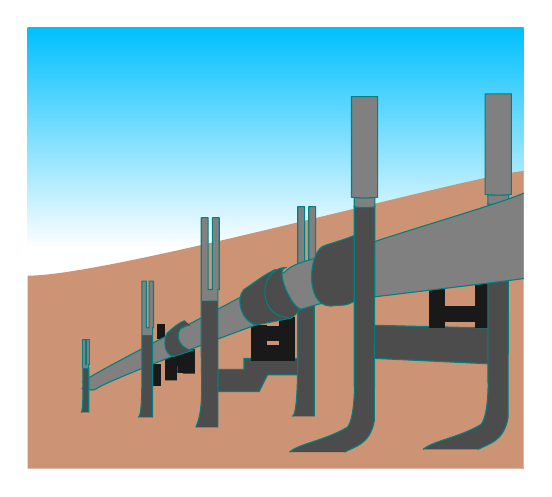
\begin{tikzpicture}[font=\footnotesize,scale=1,x=0.35cm,y=0.35cm]
		 \definecolor{antiquebrass}{rgb}{0.8,0.58,0.46}
		 \definecolor{forestgreen (web)}{rgb}{0.13,0.55,0.13}
		 \definecolor{deepskyblue}{rgb}{0.0,0.75,1.0}
		\fill[top color=deepskyblue,middle color=white]  (-9,-7) rectangle (9,9);
		\fill[antiquebrass](-9,0)..controls++(0:3) and++(-175:2)..(9,3.8)--(9,-7)--(-9,-7)--cycle; 
		\tikzset{ongdan/.pic={\draw[teal,fill=black!50] (9,3)..controls++(-150:0.5) and++(25:0.4)..(3.5,1.2)..controls++(-130:0.4) and++(45:0.7)..(0.4,0.2)..controls++(-130:0.5)  and++(40:0.7)..(-7,-3.85)..controls++(-10:0.4) and++(-170:0.3)..(-6.95,-4.1)..controls++(90:0.1) and++(-150:0.3)..(-6.5,-4.1)..controls++(40:0.5) and++(-170:1)..(1.7,-1)..controls++(10:0.3) and++(-170:0.5)..(9,-0.1);}}
		\tikzset{cot/.pic={\draw[teal,fill=black!70]  (0.5,-6.4)..controls++(40:0.5) and++(-150:1)..(2.6,-5.5)..controls++(50:0.5) and++(90:0.5)..(2.85,-4)--(2.85,2.5)..controls++(-10:0.2) and++(-170:0.2)..(3.6,2.5)..controls++(-90:0.5) and++(90:0.5)..(3.58,-5.25)..controls++(-100:0.9) and++(30:0.4)..(2.5,-6.4);
		\draw[teal,fill=black!50] (2.85,2.5)..controls++(-10:0.2) and++(-170:0.2)..(3.6,2.5)--(3.6,2.85)..controls++(-170:0.2)  and++(-10:0.2)..(2.85,2.85)--cycle;
		\draw[teal,fill=black!50] (3.7,2.85)..controls++(-170:0.2) and++(-10:0.2)..(2.75,2.85)--(2.75,6.5)--(3.7,6.5)--cycle;}} 
		\draw[teal,fill=black!70] (3.6,-1.8)--(7.8,-1.9)--(7.8,-3.2)--(3.6,-3); 
		 \tikzset{cot1/.pic={\draw[teal,fill=black!70] (-2.9,-5.6)..controls++(65:0.7) and++(-90:1)..(-2.7,-3)--(-2.7,-1)--(-2.1,-1)--(-2.1,-5.6);
		\draw[teal,fill=black!50](-2.7,-1)--(-2.7,2)..controls++(10:0.05) and++(170:0.05)..(-2.45,2)--(-2.45,-0.6)--(-2.3,-0.6)--(-2.3,2)..controls++(10:0.05)  and++(170:0.05)..(-2.05,2)--(-2.05,-0.6)--(-2.1,-0.6)--(-2.1,-1);}}
		\tikzset{cot2/.pic={\draw[teal,fill=black!70] (-2.9,-5.6)..controls++(8:0.2) and++(-90:1)..(-2.7,-3)--(-2.7,-1)--(-2.1,-1)--(-2.1,-5.6); 
		 \draw[teal,fill=black!50](-2.7,-1)--(-2.7,2)..controls++(10:0.05) and++(170:0.05)..(-2.45,2)--(-2.45,-0.6)--(-2.3,-0.6)--(-2.3,2)..controls++(10:0.05) and++(170:0.05)..(-2.05,2)--(-2.05,-0.6)--(-2.1,-0.6)--(-2.1,-1);}}
		\draw[teal,fill=black!70]  (-2.1,-3.4)--(-1.15,-3.4)--(-1.15,-3)--(1,-3)--(1,-3.6)--(-0.3,-3.6)--(-0.6,-4.2)--(-2.1,-4.2)--cycle;
		\draw[teal,black!90,line width=2mm] (0.4,-1.5)--(0.4,-2.8)--(-0.6,-2.8)--(-0.6,-1.8) 
			 (-0.6,-2.1)--(0.4,-2.1);
		\draw[teal,black!90,line width=2mm]  (5.85,-0.5)--(5.85,-1.9)
			(7.5,-0.3)--(7.5,-1.9) 
			 (5.85,-1.4)--(7.5,-1.4);
		\draw[teal,black!90,line width=1.5mm]  (-3.8,-2.95)--(-3.8,-3.8)
			 (-3.15,-2.66)--(-3.15,-3.55)
			(-3.35,-2.7)--(-3.35,-3.53) 
			 (-3.8,-3.1)--(-3.15,-3);
		\draw[teal,black!90,line  width=1mm] (-4.3,-4)--(-4.3,-3.2)
			 (-4.15,-2.3)--(-4.15,-1.75);
		\path  (3.5,0.5) pic[scale=1]{cot2};
		\path  (4.85,0.1) pic[scale=1]{cot};
		 \path (0,0) pic[scale=1]{ongdan};
		\draw[teal,fill=black!70]  (1.8,1.1)..controls++(-170:0.6) and++(180:1)..(2,-1.1)..controls++(10:0.4) and++(-150:0.5)..(2.9,-0.9)..controls++(90:0.3) and++(-90:0.3)..(3.1,1.6)..controls++(-140:0.3) and++(20:0.3)..(1.8,1.1);
		\path  (0,0.1) pic[scale=1]{cot1};
		\path  (-3.1,-1.5) pic[scale=0.65]{cot2};
		\path  (0,0) pic[scale=1]{cot};
		\path (-6.05,-3)  pic[scale=0.35]{cot2};
		\path  (-6,1) node[rotate=12]{};
		\draw[teal,fill=black!70](0,0.23)..controls++(-155:0.4) and++(35:0.4)..(-1,-0.4)..controls++(-160:0.5)  and++(160:0.7)..(-0.73,-1.79)--(0.5,-1.55);
		\draw[teal,fill=black!70]  (0.4,0.3)..controls++(180:1) and++(170:1)..(0.3,-1.5)..controls++(0:0.2) and++(-130:0.7)..(0.9,-1.2)..controls++(180:0.3) and++(180:0.5)..(0.4,0.3);
		 \draw[teal,fill=black!70] (-3.1,-1.8)..controls++(180:0.7) and++(180:0.6)..(-3,-2.7)--(-3.7,-2.93)..controls++(170:0.4) and++(-120:0.2)..(-3.95,-2.1)..controls++(45:0.3) and++(-160:0.2)..(-3.3,-1.63);
		\path (6.5,0.8)  node[yellow,rotate=13]{};
	\end{tikzpicture}
	} 
	\noindent 
	Vì địa hình  phức tạp, người ta chọn điểm $A(15;10;15)$ để làm điểm trung chuyển đầu từ mặt đất đến đường ống này.
	\choiceTF 
		{\True Đường  ống dẫn dầu nằm trên mặt phẳng $(Oyz)$}
		{Điểm đối xứng với $A$ qua mặt  phẳng $(Oxy)$ có tọa độ $A'(-15;-10;15)$}
		{\True Do thực tế công việc, người ta cần xác định vị trí điểm $B(0;b;20)$ thuộc đường ống và vị trí điểm $C(m;n;0)$ thuộc mặt đất sao cho tổng độ  dài các đoạn đường $AB$, $BC$, $AC$ nhỏ nhất. Khi đó $m+n+b = \dfrac{200}{7}$}
		{Giá trị nhỏ  nhất của tổng độ dài các đoạn thẳng $AB$, $BC$, $AC$ làm tròn đến hàng chục bằng $45{,}5$ m}
	\loigiai{ 
		\begin{itemchoice}
			\itemch Mọi điểm $M$ thuộc  đường ống dẫn dầu $d$ đều có dạng $M\left(0;t;20\right)$ với $t\in \mathbb{R}$.\\
			Mà  $(Oyz)\colon x=0$ nên $M\in (Oyz)$.\\
			Suy ra mọi điểm  trên đường ống dẫn dầu đều nằm trên mặt phẳng $(Oyz)$.\\
			Vậy  đường ống dẫn dầu nằm trên mặt phẳng $(Oyz)$.
			\itemch Điểm  đối xứng của $A(15;10;15)$ qua mặt phẳng $(Oxy)$ là $A'(15;10;-15)$.
			\itemch Đặt tổng độ dài  các đoạn đường $AB$, $BC$, $AC$ là $T=AB+BC+AC=AB+CB+CA'$.\\
			Ta  có $T$ đạt giá trị nhỏ nhất khi và chỉ khi $AB_{\min\limits}$ và $\left( CB+CA' \right)_{\min\limits}$.\\
			Ta có $AB=\sqrt{\left(0-15\right)^2 + \left( b-10\right)^2 + (20-15)^2  }=\sqrt{250+(b-10)^2}$.\\
			Khi đó $AB_{\min\limits}=\sqrt{250}=5\sqrt{10}$ khi và chỉ khi $b=10$. Suy ra $B(0;10;20)$.\\ 
			Ta có $CB+CA'\geq  CA'$. Do đó $\left( CB+CA' \right)_{\min\limits}=BA'$ khi và chỉ khi $C$, $B$, $A'$ thẳng hàng.\\
			Ta có $\overrightarrow{CB}=(-m;10-n;20)$, $\overrightarrow{CA'}=(15-m;10-n;-15)$.\\ 
			Ta có $C$, $B$, $A'$ thẳng hàng khi và chỉ khi $\overrightarrow{CB}$ cùng phương $\overrightarrow{CA'}$ khi và chỉ khi tồn tại số thực $k$ sao cho 
			\begin{eqnarray*}
				\overrightarrow{CB} =k\cdot \overrightarrow{CA'}\Leftrightarrow 
				\heva{&-m=k\cdot (15-m)\\&10-n=k\cdot  (10-n)\\
				&20=k\cdot(-15) }  \Leftrightarrow
				\heva{&m=\dfrac{60}{7}\\&n=10\\&k=-\dfrac{4}{3}.} 
			\end{eqnarray*}
			 Suy ra $C\left( \dfrac{60}{7}; 10; 0 \right)$.\\
			Vậy $m+n+b=\dfrac{60}{7}+10+10=\dfrac{200}{7}$. 
			\itemch Ta có $T=AB+BC+AC$ nhỏ nhất khi và chỉ khi $B(0;10;20)$, $C\left(\dfrac{60}{7}; 10;  0 \right)$.\\
			Ta có  $AB=5\sqrt{10}$, $BC=\dfrac{20\sqrt{58}}{7}$, $AC=\dfrac{15\sqrt{58}}{7}$.\\
			Suy ra $T_{\min\limits}=5\sqrt{10} + \dfrac{20\sqrt{58}}{7} +  \dfrac{15\sqrt{58}}{7} \approx 53{,}9$ m.
		\end{itemchoice}
	 }
\end{ex}

% nguồn: Phan1_Lop_12_Hinh_hoc_Chuong_5
\begin{ex}%[2H5V2-8]%[ma:f76e5611]
	Trong không gian với hệ trục tọa độ $Oxyz$, xét mô hình phòng không như sau: Rađa đặt tại gốc toạ độ $O(0;0;0)$, tên lửa phòng không đặt tại điểm $A(0;100;0)$; mỗi đơn~vị trên mỗi trục tọa độ tương ứng với $10~\mathrm{m}$; mặt phẳng $(Oxy)$ trùng với mặt đất; giả sử mọi UAV (phương tiện bay không người lái) và tên lửa đều chuyển động thẳng đều. Tại thời điểm $t=0$ giây, rađa phát hiện ra UAV $M$ ở tọa độ $M_0(20\,000;0;20)$; tại thời điểm $t=1$ giây, rađa theo dõi thấy  UAV $M$ ở toạ độ $M_1(19\,995;1;19{,}5)$. Gọi $d$ là đường thẳng qua $M_0$, $M_1$.
	 \choiceTF
		{Góc nghiêng của đường thẳng $d$  và mặt đất là $0{,}02~\mathrm{rad}$}
		{Khoảng cách giữa UAV $M$ và gốc $O$ tại  thời điểm $6$ giây là $19\,970$ m}
		{\True Khoảng cách ngắn nhất từ điểm $A$ tới đường thẳng $d$ xấp xỉ $42\,684$ m} 
		{\True Tại thời điểm $t=6$ giây, một tên lửa được phóng lên từ $A$  và chuyển động thẳng đều với vận tốc $3\,400~\mathrm{m/s}$, va chạm và phá huỷ UAV $M$ tại điểm $B$ trên $d$. Khi đó, sau $57{,}88$ giây kể từ lúc phóng thì tên lửa va chạm với UAV (kết quả làm tròn đến hàng phần trăm của giây)}
		\begin{center}
			\begin{tikzpicture}[font=\footnotesize,line join=round,line cap=round,>=stealth]
					\path (0:0) coordinate (O)--++(90:.8) coordinate (Z) node[above left]{$20$}--++(90:.9)  coordinate (z) node[left]{$z$}
						(O)--++(0:1) coordinate (A) --++(0:2) coordinate (y)  node[below]{$y$}--++(-150:4) coordinate (B)
						 (O)--++(-140:4) coordinate (X) node[below right]{$20\,000$}--++(-140:.6) coordinate (x) node[left]{$x$};
					\draw ($(X)+(Z)-(O)$) coordinate (M); 
					 \draw ($(M)!-.2!(B)$) --($(M)!1.2!(B)$) node[below]{$d$}
						 (A)--(B);
					\draw[dashed]  (Z)--(M)--(X);
					\draw[->] (O)--(z); 
					 \draw[->] (O)--(x);
					\draw[->] (O)--(y); 
					 \foreach \x/\g in {A/90,B/-90,O/-70,M/98}
					 \fill (\x) circle (1pt)
						($(\x)+(\g:3mm)$)  node{$\x$};
					\fill (X)  circle (1pt);
					\fill (Z) circle  (1pt);
				\end{tikzpicture}
	\end{center}
	\loigiai{ 
		\begin{itemchoice}
			\itemch Ta có  $\overrightarrow{M_0 M_1}=(-5;1;-0{,}5)$ là một vectơ chỉ phương của $d$ và một vectơ pháp tuyến của mặt phẳng $(Oxy)$ là $\overrightarrow{k}=(0;0;1)$.\\
			Khi đó $\sin \left(d,(Oxy)\right)  =\dfrac{|-0{,}5|}{\sqrt{5^2+1^2+0{,}5^2} \cdot 1}=\dfrac{1}{\sqrt{105}}$.\\
			Suy ra $\left(d,(Oxy)\right) \approx  0{,}098 \mathrm{~rad}$.
			\itemch Phương trình tham số của đường thẳng $d$ là $\left\{\begin{array}{l}x=20\,000-5t \\ y=t \\ z=20-0{,}5 t.
		\end{array}\right.$\\
		Do UAV chuyển động thẳng đều nên ta có thể đồng nhất $t$ với số giây  bay được của UAV, tính từ lúc nó bị rađa phát hiện. Toạ độ của UAV lúc $6$ giây là $M_6(19\,970;6;17)$.\\
		Suy  ra $OM_6 \approx 19\,970$.\\
		Vậy khoảng cách thực tế là $199\,700$ m (do quy đơn~vị $1$  đơn~vị tọa độ bằng $10$ m).
		 \itemch Ta có
		\allowdisplaybreaks 
		\begin{align*}
			MA&=\,\sqrt{(20\,000-5 t)^2+(100-t)^2+(20-0{,}5 t)^2}\\ 
			&=\,\sqrt{26{,}25  t^2-200\,220 t+400\,010\,400} \geq 4\,268{,}4.
		\end{align*}
		Vậy khoảng cách ngắn nhất  từ $A$ tới $d$ là $42\,684$ m.
		\itemch Tốc độ $(10 \mathrm{~m}/\mathrm{s})$  của UAV là $v_1=\dfrac{M_1 M_0}{1}=\sqrt{26{,}25}$.\\
		Tốc độ của tên lửa $(10\mathrm{~m}/\mathrm{s})$  là $v_2=340$.\\
		Mặt khác, toạ độ $B$ có dạng $B(19\,970-5 a;6+a;17-0{,}5a)$ với $a\geq 0$, $a=0$ tính từ lúc UAV đi qua điểm $M_6$.\\ 
		Tên  lửa va chạm và phá huỷ UAV tại $B$, tức là $\dfrac{M_6B}{v_1}=\dfrac{AB}{v_2}$.\\
		Từ đó ta  có
		\allowdisplaybreaks 
		\begin{align*}
			&\dfrac{\sqrt{(5a)^2+a^2+(0{,}5  a)^2}}{\sqrt{26{,}25}}=\dfrac{\sqrt{(19\,970-5 a)^2+(a-94)^2+(17-0{,}5 a)^2}}{340} \\
			 \Leftrightarrow&\, 340a=\sqrt{(19\,970-5 a)^2+(a-94)^2+(17-0{,}5 a)^2} \\
			\Leftrightarrow&\, 115\,573{,}75 a^2+199\,905 a-398\,810\,025=0\\ \Leftrightarrow&\,  a \approx 57{,}88.
		\end{align*}
		Vậy sau $57{,}88$ giây kể từ lúc phóng thì tên lửa va chạm với UAV. 
	\end{itemchoice}
	} 
	\end{ex}

% nguồn: Phan1_Lop_12_Hinh_hoc_Chuong_5
\begin{ex}%[2H5V2-8]%[ma:c47ef310]
	 Một radar phòng không được đặt tại vị trí gốc tọa độ $O(0;0;0)$ trong không gian $Oxyz$, mỗi đơn vị trên các trục tọa độ ứng với $1$ km. Radar này có khả năng phát hiện các mục tiêu bay trong bán kính $250$ km. Một máy bay không người lái (UAV) đang bay thẳng đều từ vị trí điểm $A(300;-400;100)$ đến điểm $B(-300;400;100)$. UAV bay với vận tốc không đổi $900$ km/h và mang theo thiết bị gây nhiễu chủ động có tầm hiệu quả $50$ km tính tử UAV.
	\begin{flushright}
		(Tham khảo từ  Stimson's Introduction to Airborne Radar, $3$rd Edition,
		 George W. Stimson, Hugh D. Griffiths, Christopher Baker, Dave Adamy)
	\end{flushright}
	 \choiceTF
		{\True Radar không thể phát hiện UAV khi UAV ở vị trí  $A$}
		{Phương trình tham số của đường bay của  UAV là $\heva{&x=300-3t \\ &y=-400+4t,t \in \mathbb{R}\\ &z=0}$}
		{Trong suốt quá trình bay, sẽ có thời điểm UAV gây nhiểu được  radar}
		{\True Radar có thể theo dõi UAV trong khoảng thời gian hơn  $30$ phút}
	\loigiai{ 
		\begin{itemchoice}
			\itemch Do $OA=100 \sqrt{26}>250$ nên radar không thể phát hiện UAV khi UAV ở vị  trí $A$.
			\itemch Ta có đường bay của UAV đi qua $A(300;-400;100)$ và nhận $\vec{u}=(-3;4;0)$ cùng phương với  $\overrightarrow{AB}=(-600;800;0)$ làm một véc-tơ chỉ phương.\\
			Suy ra phương trình  tham số của đường bay UAV là
			$$AB\colon\heva{ 
			&x=300-3  t \\
			&y=-400+4t,t  \in \mathbb{R}.\\
			 &z=100}$$
			\itemch Vì $\mathrm{d}(O, AB)=\dfrac{\left|\left[\vec{u}, \overrightarrow{O A}\right]\right|}{\left|\vec{u}\right|}=\dfrac{500}{5}=100>50$ nên trong suốt quá trình bay, sẽ không có thời điểm  nào UAV gây nhiễu được radar.
			\itemch \begin{center}
			\begin{tikzpicture}[scale=.75,font=\footnotesize,line join=round,line cap=round,>=stealth]
					 \def\r{5}
					\coordinate (O) at  (0,0);
					\coordinate (N)  at ($(O)+(45:\r)$);
					\coordinate (M) at  ($(O)+(150:\r)$);
					\coordinate (H) at ($(M)!(O)!(N)$); 
					\draw[teal]  (O) circle (\r cm);
					 \draw[teal] (\r,0) arc (0:-180:\r cm and 1cm);
					\draw[teal,dashed] (\r,0) arc (0:180:\r cm and  1cm);
					\draw[teal,dashed] (-\r,0)--(\r,0) 
						(M)--(N)--(O) node[midway,below]{$250$}--cycle (O)--(H) node[midway,right]{$100$}; 
					\draw[teal] pic[draw,angle  radius=2mm]{right angle=O--H--N};
					 \foreach \p/\r in {O/-90,M/150,N/45,H/90}
					 \fill (\p) circle (1.2pt) node[shift={(\r:3mm)}]{$\p$};
				\end{tikzpicture}
		\end{center}
		Mô phỏng như hình vẽ, trong khoảng thời  gian $30$ phút ta có\\
		 Quãng dường Rada có thể theo dõi UAV là $MN=2HN=2\sqrt{250^2-100^2}=100\sqrt{21}$.\\
		Suy ra thời gian Radar có thể theo dõi UAV là $\dfrac{100 \sqrt{21}}{900}  \approx 0{,}509>0{,}5$ giờ.\\
		Vậy Radar có thể theo dõi UAV  trong khoảng thời gian hơn $30$ phút.
	\end{itemchoice}
 }
\end{ex}

% nguồn: Phan1_Lop_12_Hinh_hoc_Chuong_5
\begin{ex}%[2H5V2-8]%[ma:b1b42c04]
	Một căn phòng khách có hình dạng là một hình hộp chữ nhật được gắn trong hệ trục toạ độ $Oxyz$ với các  thông số như hình bên (đơn~vị trên mỗi trục là mét). Coi mặt sàn nằm trên mặt phẳng $(Oxy)$. Theo thiết kế, chủ nhà muốn trang trí một đèn pha lê hình cầu có bán kính $15$ cm được nối với trần nhà ở vị trí điểm $H$ bởi một dây dài $1$ m ($H$ là trung điểm của $EF$, biết $EF\parallel PQ$ và $QF=4$ m, hình bên).
	\begin{center}
		\begin{tikzpicture}[font=\footnotesize,line join=round,line cap=round,>=stealth]
				\def\a{5} 
				\def\b{1} 
				 \def\g{30}
				 \def\h{2}
				\path (0:0) coordinate (A)--++(\g:\b) coordinate (B)--++(0:\a) coordinate (C)--++(\g-180:\b)  coordinate (D)
				\foreach \x in {A,B,C,D}{($(\x)+(90:\h)$)  coordinate (\x')};
				\draw[dashed] (B') node[above left]{$M$}--(B) node[left]{$O$}--(A)  node[below]{$A$}
					(B)--(C) node[above  right]{$C$};
				 \draw (D) node[below]{$B$}--(D') node[below left]{$P$}
					(A') node[left]{$N$}--(B')--(C')  node[right]{$Q$}--(D')--(A')--(A)--(D)--(C)--(C');
				\draw ($(B')!.6!(C')$) coordinate (F) node[above]{$F$} --($(A')!.6!(D')$)  coordinate (E) node[below]{$E$}
					($(E)!.5!(F)$)  coordinate (H);
				\draw[dashed] (H) node[left]{$H$}--($(H)+(0,-1)$) coordinate  (G);
				\fill[ball color=blue]  (G) circle (5pt);
				\foreach \diem/\anh/\ts in {A/x/1.5,C/y/1.1,B'/z/1.4} \coordinate (\anh) at  ($(B)!\ts!(\diem)$);
				\draw ($(A)!.5!(A')$)  node[left]{$4$ m}
					($(A)!.5!(D)$)  node[below]{$10$ m}
					($(D)!.5!(C)$)  node[below right]{$4$ m}
					($(F)!.5!(C')$)  node[above]{$4$ m}
					($(F)!.5!(H)$)  node[right=2pt]{$2$ m};
				\draw[->](B')--(z) node[left]{$z$}; 
				\draw[->](A)--(x) node[left]{$x$}; 
				 \draw[->](C)--(y) node[below]{$y$};
				 \foreach \x in {A,B,C,D,A',B',C',D',E,F,H}
				 \fill (\x) circle (1pt);
			\end{tikzpicture}
	\end{center}
	\choiceTF 
		{Cao độ tâm  $I$ của đèn pha lê hình cầu là $3$}
		{Phương trình mặt cầu của đèn pha lê là $(x-2)^2+(y-6)^2+(z-3)^2=0{,}0225$} 
		{Một người cao $1{,}8$ m thì khi đi ngang qua phía dưới sẽ cách đèn ít nhất là $60$  cm}
		{\True Tia sáng từ tâm đèn chiếu ra cắt sàn nhà tại $K$. Khoảng cách xa nhất từ $K$ tới $B$ là khoảng $10{,}77$ m (kết quả làm tròn  đến hàng phần trăm)}
	 \loigiai{
	\begin{itemchoice}
		\itemch Khoảng cách từ mối nối sợi dây và đèn pha lê đến sàn nhà  là $4-1=3$ m.\\
		Đèn pha lê có bán  kính $15 \mathrm{~cm}=0{,}15 \mathrm{~m}$ nên khoảng cách từ tâm đèn đến sàn nhà là $3-0{,}15=2{,}85\mathrm{~m}$.\\
		Vậy cao  độ tâm $I$ của đèn hình cầu là $2{,}85$ m.
		\itemch 
		Ta có $M F=10-4=6$ m nên tâm  $I$ của đèn hình cầu có tọa độ là $I(2;6;2{,}85)$.\\
		Do đó phương trình  mặt cầu của đèn pha lê là $(x-2)^2+(y-6)^2+(z-2{,}85)^2=0{,}0225$.
		 \itemch
		Vị trí thấp nhất của đèn cách sàn  nhà là $3-0{,}15 \cdot 2=2{,}7\mathrm{~m}$.\\
		Ta có $2{,}7-1{,}8=0{,}9\mathrm{~m}=90\mathrm{~cm}$ nên  một người cao $1{,}8 \mathrm{~m}$ khi đi ngang qua phía dưới sẽ cách đèn ít nhất $90$ cm.
		\itemch Khoảng cách xa nhất từ $K \equiv O$ tới $B$ là $\sqrt{10^2+4^2}=2  \sqrt{29} \approx 10{,}77$ m.
	\end{itemchoice}
	 }
\end{ex}

% nguồn: Phan1_Lop_12_Hinh_hoc_Chuong_5
\begin{ex}%[2H5V2-8]%[ma:74aeafbb]
	Một cáp treo xuất phát từ điểm $A(10;3;0)$ và chuyển động  đều theo đường cáp có vectơ chỉ phương $\overrightarrow{u}=(2;-2;1)$ với tốc độ là $4{,}5\mathrm{~m}/\mathrm{s}$ (đơn~vị trên mỗi trục là mét) được mô hình hoá như các hình vẽ sau:
	\begin{center}
		\begin{tikzpicture}[scale=0.7,font=\footnotesize,line join=round,line cap=round,>=stealth]
				\draw[->]  (0:0) coordinate (O)--++(0:4) coordinate (y) node[below=-2pt]{$y$};
				\draw[->] (O)  node[above right=-2pt]{$O$}--++(90:4) coordinate (z) node[left]{$z$};
				 \draw[->] (O)--++(-140:5) coordinate (x) node[left=-2pt]{$x$};
				\path (O)--++(0:1) coordinate (E)--++(-140:2) coordinate  (A) node[below=-2pt]{$A (10; 3; 0)$}--++(180:1) coordinate (F);
				\draw[dashed]  (E)--(A)--(F);
				\draw[->]  (O)--++(145:1.5) coordinate (n) node[above=-2pt]{$\overrightarrow{u}$};
				 \draw ($(A)+(n)-(O)$) coordinate (b);
				\draw ($(A)!2.3!(b)$) coordinate (B) node[above=-2pt]{$B$}; 
				\draw (B)--++(-90:3.5) node[below  right=-2pt]{$x_B=550$};
				\draw ($(A)!.6!(B)$)  coordinate (M) node[below left=-2pt]{$M$};
				 \draw (A)--(B);
				 \foreach \i in {A,B,O,M} \fill (\i) circle (1pt);
			\end{tikzpicture}
	\end{center}
	 \choiceTF
		{\True Phương trình  chính tắc của đường cáp là $\dfrac{x-10}{2}=\dfrac{y-3}{-2}=\dfrac{z}{1}$}
		{\True Giả sử  sau $t$ giây kể từ lúc xuất phát $t>0$, cabin đến vị trí điểm $M$. Khi đó tọa độ của điểm $M$ là $\left(3t+10;-3t+3;\dfrac{3t}{2}\right)$}
		{\True Cabin dừng ở  điểm $B$ có hoành độ $x_B=550$. Quãng đường $AB$ có độ dài bằng $810 \mathrm{~m}$}
		{Đường cáp $AB$ tạo với mặt phẳng $Oxy$ một góc $22^{\circ}$ (làm tròn đến hàng đơn~vị theo  độ)}
	\loigiai{ 
		\begin{itemchoice}
			\itemch Vì đường cáp đi qua  điểm $A(10;3;0)$ có vectơ chỉ phương $\overrightarrow{u}=(2;-2;1)$ nên có phương trình chính tắc là $\dfrac{x-10}{2}=\dfrac{y-3}{-2}=\dfrac{z}{1}$.
			\itemch Sau $t$ giây kể từ lúc xuất phát $t>0$, cabin đến vị trí điểm  $M$. Khi đó cabin đi được đoạn đường có độ dài bằng đoạn $AM=4{,}5 t$.\\
			Đặt $\dfrac{x-10}{2}=\dfrac{y-3}{-2}=\dfrac{z}{1}=u \Rightarrow\left\{\begin{aligned}&x=10+2 u \\ &y=3-2 u \\ &z=u.
		\end{aligned}\right.$\\
		Suy  ra toạ độ điểm $M$ là $M(10+2u;3-2u;u)$, $u>0$.\\
		 Khi đó $AM=4{,}5 t \Leftrightarrow 2 u^2+2 u^2+u^2=4{,}5 t^2 \Leftrightarrow 9 u^2=\dfrac{81}{4} t^2$.\\
		Vì $u>0$ nên $u=\dfrac{3}{2}t$.\\ 
		Vậy $M\left(10+3t;3-3t;\dfrac{3}{2}  t\right)$.
		\itemch  Ta có $B(10+2u;3-2u;u)$, $u>0$.\\
		Vì $B$  có hoành độ $x_B=550$ nên $10+2u=550 \Rightarrow u=270$.\\
		Từ đó  có $B(550;-537;270)$. Suy ra $AB=810$\,m.
		\itemch Đường cáp $AB$ có  một vectơ chỉ phương $\overrightarrow{u}=(2;-2;1)$, mặt phẳng $Oxy$ có một vectơ pháp tuyến là $\vec{k}=(0;0;1)$.\\
		Suy ra góc giữa đường cáp $AB$ và mặt phẳng $Oxy$ là $\varphi$ với $$\sin \varphi=\dfrac{\left|\overrightarrow{u} \cdot \overrightarrow{k}\right|}{\left| \overrightarrow{u}\right| \cdot\left|\overrightarrow{k}\right|}=\dfrac{1}{3} \Rightarrow \varphi \approx 19^{\circ}.$$ 
	\end{itemchoice}
	} 
	\end{ex}

% nguồn: Phan1_Lop_12_Hinh_hoc_Chuong_5
\begin{ex}%[2H5V2-8]%[ma:a7c392ad]
	\immini{Khi gắn hệ tọa độ $Oxyz$ (đơn~vị trên mỗi trục tính theo kilômét) vào một sân bay, mặt phẳng $(Oxy)$ trùng với mặt sân bay, một máy bay đang  ở vị trí $A(4;-5;1)$ sẽ hạ cánh khẩn cấp ở vị trí $B(1;2;0)$ trên đường băng $EG$.
	 \choiceTF
		{\True Phương trình đường thẳng $AB$  là $\heva{&x=4-3t \\ &y=-5+7t \\ &z=1-t}$ ($t$ phút)}
		{Góc trượt (góc giữa đường  bay $AB$ và mặt đất là mặt phẳng nằm ngang $(Oxy)$) không nằm trong phạm vi cho phép từ $2{,}5^\circ$ đến $9^\circ$}
		{\True Có một lớp mây mô phỏng bởi mặt phẳng $(P)$ đi qua ba điểm $M(5;0;0)$, $N(0;-1;0)$, $P\left(0;0;2\right)$. Máy  bay xuyên qua đám mây tại điểm $C$ có độ cao làm tròn đến hàng đơn~vị là $346$ m}
		{\True Biết rằng tầm nhìn của người phi công sau khi ra khỏi đám mây là $800$ m. Sau khi ra khỏi đám mây, người phi công đạt được quy định an toàn bay là người  phi công phải nhìn thấy điểm đầu $E(2;0{,}5;0)$ của đường băng ở độ cao tối thiểu $150 $ m}}{
	\def\hinhabm{
\begin{tikzpicture}[line cap=round,line join=round]
		\path[fill,rounded  corners=9pt] (12.5,5) rectangle +(3.5,2.4)
			(12.5,-5)  rectangle +(3.5,-2.4);
		\def\canhtren{(13.3,0).. controls +(0:0) and +(-58:1.8).. 
			(8.36,9.19)..  controls +(122:2.4) and +(136:1.8)..
			(9.96,10.79).. controls  +(-44:1.8) and +(0:0)..
			 (19.96,0)}
		\path[top color=cyan!80!blue,bottom color=cyan!90!black] \canhtren; 
		\path[bottom color=cyan!80!blue,top color=cyan!90!black,yscale=-1] \canhtren; 
		\def\canhsau{(1.66,0).. controls  +(0:0) and +(-90:0.8)..
			(0.83,4.16)..  controls +(90:0.8) and +(135:1.2)..
			(2.49,4.99).. controls +(-45:1.2) and  +(0:0)..
			 (6.65,0)}
		\path[top color=cyan!80!blue,bottom color=cyan!90!black] \canhsau; 
		\path[bottom color=cyan!80!blue,top color=cyan!90!black,yscale=-1]  \canhsau;
		 \path[bottom color=gray!80,top color=gray!80,middle color=gray!65] (20.79,2.49).. controls +(0:1.7) and +(90:0.8)..
			(24.95,0).. controls +(-90:0.8)  and +(0:1.7)..
			(20.79,-2.5).. controls +(180:1.7)  and +(0:0)..
			(5.4,-2.08)..  controls +(0:0) and +(-90:1.2)..
			(0.83,0).. controls  +(90:1.2) and +(0:0)..
			(5.4,2.08).. controls +(0:0) and  +(180:1.7)..
			(20.79,2.5) --cycle; 
		 \path[fill=gray!60!black]
			(21.2,1.25)  arc (-45:45:1.76 and -1.76) -- (21.54,-1.58).. controls +(24:0.2) and +(-133:0.2)..
			(22.03,-1.25) arc (45:-45:1.76 and -1.76)..  controls (21.89,1.39) and (21.72,1.5)..
			(21.54,1.58)  --cycle
			(7.48,0)..  controls +(0:0) and +(0:3.7)..
			(3.74,-0.42).. controls +(180:3.7)  and +(0:0)..
			(0,0).. controls  +(0:0) and +(180:3.7)..
			(3.74,0.41).. controls +(0:3.7)  and +(0:0)..
			(7.48,0)  --cycle;
	\end{tikzpicture}
		 }
		\begin{tikzpicture}[scale=0.5,line join=round]
				\path  (-3,2.5) coordinate (O)
					(-9,2.5) coordinate (x') 
					(6,2.5)  coordinate (x)
					(-3,2.5) coordinate  (y')
					 (-3,6.5) coordinate (y)
					 (-6,-1.5) coordinate (z);
				\path ($(O)!0.5!(z)$)  coordinate (M);
				\path ($(O)!(M)! (x)$) coordinate (N); 
				 \path ($(N)-(M)+(O)$) coordinate (P);
				\path  (0,-1.5) coordinate (E)
					(3,-1.5) coordinate  (B)
					(9,-1.5) coordinate  (G)
					(-6,5.5) coordinate (A); 
				\draw[-stealth]  (O)--(x) node[below]{$y$};
				\draw[-stealth]  (y')--(y) node[right]{$z$};
				\draw[-stealth] (y')--(z) node[right]{$ $}; 
				\draw (x')--(N); 
				\draw[dashed]  (N)--(O);
				 \draw (M)--(N)--(P)--(M)
					(E)--(B)--(G); 
				\foreach \x/\y in {O/-45,M/180,N/140,P/0,E/90,G/90} 
				\fill[cyan]  (\x) circle (1pt)
					 ($(\y:9pt)+(\x)$) node {$\x$};
				\foreach  \x/\y in {B/90,A/90}
				 \fill (\x) circle (1pt)
					($(\y:9pt)+(\x)$) node  {$\x$};
				\path (A)--(B) node[sloped,pos=0.65]{\resizebox{!}{2cm}{ 
				 \hinhabm
					 }};
			\end{tikzpicture}
		 }
	 \loigiaiDS{
		\begin{itemchoice}
			\itemch Ta có $\overrightarrow{AB}=(-3;7;-1)$.\\ 
			Đường thẳng $AB$ đi qua điểm $A(4;-5;1)$ và có một vectơ chỉ phương $\overrightarrow{AB}=(-3;7;-1)$ nên phương trình tham số của đường thẳng $AB$ là  $\heva{&x=4-3t \\ &y=-5+7t \\ &z=1-t}$ ($t$ phút).
			\itemch 
			Mặt  phẳng $(Oxy)$ có một véc-tơ pháp tuyến $\vec{k}=(0;0;1)$.\\
			Ta có 
			\begin{align*}
				 \sin \left(AB,(Oxy)\right)&=\left|\cos (\overrightarrow{AB},\vec{k})\right|\\
				&=\dfrac{\left|(-3)\cdot  0+7\cdot 0+(-1)\cdot 1\right|}{\sqrt{(-3)^2+7^2+(-1)^2}\cdot\sqrt{0^2+0^2+1^2}}\\
				 &=\dfrac{1}{\sqrt{59}}.
			\end{align*}
			Suy ra  $\left(AB,(Oxy)\right)\approx 7{,}5^\circ$.
			 Vậy góc trượt (góc giữa đường bay $AB$ và mặt đất là mặt phẳng nằm ngang $(Oxy)$) có nằm trong phạm vi cho phép từ $2{,}5^\circ$ đến $9^\circ$.
			\itemch Mặt phẳng $(P)$ đi qua ba điểm $M(5;0;0)$, $N(0;-1;0)$, $P(0;0;2)$ nên mặt phẳng $(P)$ có phương  trình là $\dfrac{x}{5}+\dfrac{y}{-1}+\dfrac{z}{2}=1\Leftrightarrow 2x-10y+5z-10=0$.\\
			Điểm $C$ thuộc đường thẳng $AB$  nên $C(4-3t;-5+7t;1-t)$.\\
			Máy bay xuyên qua đám mây $(P)\colon 2x-10y+5z-10=0$ tại điểm $C(4-3t;-5+7t;1-t)$ nên ta  có $2(4-3t)-10(-5+7t)+5(1-t)-10=0\Leftrightarrow 81t=53\Leftrightarrow t=\dfrac{53}{81}$.
			Vậy $C\left(\dfrac{55}{27};-\dfrac{34}{81};\dfrac{28}{81} \right)$.\\ 
			 Vậy máy bay xuyên qua đám mây tại điểm $C$ có độ cao $\dfrac{28}{81}$ km $\approx 346 $ m.
			 \itemch
			Máy bay cách mặt đất với độ cao $150 $  m nên $1-t=0{,}15\Leftrightarrow t=0{,}85$. Vậy $D(1{,}45;0{,}95;0{,}15)$.\\
			Ta  có $\overrightarrow{DE}=(-0{,}55;-0{,}45;-0{,}15) \Rightarrow DE=\sqrt{(-0 {,}55)^2+(-0{,}45)^2+(-0{,}15)^2} \approx 726$ m $ < 800$ m.\\
			Vậy người phi công đạt được quy định an toàn bay là người phi công phải nhìn thấy điểm đầu $E(2;0,5;0)$ của đường băng ở độ  cao tối thiểu $150$ m.
		\end{itemchoice}
	} 
\end{ex}

% nguồn: Phan1_Lop_12_Hinh_hoc_Chuong_5
\begin{ex}%[2H5V2-8]%[ma:27b4d413]
	\immini[thm]{Một chiếc máy bay thương mại Comac C$919$ đang bay trên bầu trời theo một đường thẳng từ $D$ đến $E$ có hình chiếu trên mặt đất là đoạn $CB$. Tại vị trí $D$ thì máy bay bay cách mặt đất $9\,000$\,m, tại vị trí $E$ thì máy bay cách mặt đất $12\,000$\,m. Một ra đa được đặt trên mặt đất tại vị trí $O$ cách $C$ khoảng $20\,000$\,m, cách $B$ khoảng $16\,000$\,m và $\widehat{BOC}=90^{\circ}$; phạm vi theo dõi của rađa là $20$\,km. Xét hệ trục tọa  độ $Oxyz$ (đơn vị trên mỗi trục là $1\,000$\,m) với $O$ là vị trí đặt ra đa, $B$ thuộc tia $Oy$, $C$ thuộc tia $Ox$.}
	 {
	\begin{tikzpicture}[scale=0.6,font=\footnotesize,line join=round,line cap=round,>=stealth]
			 \tikzset{MayBay/.pic={
			\begin{scope}
				\draw[teal] (-8.14,0.88)..controls++(9.87:0.42)  and++(222.06:0.26)..(-7.12,0.82)..controls++(22.47:0.35) and++(209.19:1.13)..(-6.47,0.97)..controls++(15.84:0.62) and++(25.26:0.77)..(-6.56,0.57)..controls++(224.13:0.07) and++(221.73:0.17)..(-6.41,0.52)..controls++(1.09:0.07) and++(19.23:0.22)..(-6.47,0.34)..controls++(308.61:0.44) and++(335.04:0.39)..(-6.73,0.24)..controls++(199.4:0.12) and++(243.97:0.14)..(-6.84,0.3)..controls++(192.06:0.4) and++(19.61:0.83)..(-7.35,0.22)..controls++(198.78:0.14) and++(129.96:0.2)..(-7.52,0.09)..controls++(211.53:0.07) and++(21.46:0.25)..(-7.92,0.11)..controls++(145.89:0.15) and++(347.01:0.59)..(-8.21,0.31)..controls++(62.65:0.07) and++(344.74:0.02)..(-7.85,0.29)..controls++(47.6:0.08) and++(301.95:0.48)..(-7.89,0.58)..controls++(359.29:0.01) and++(159.44:0.02)..(-7.83,0.61)..controls++(323.66:0.34) and++(208.66:0.32)..(-7.34,0.49)..controls++(92.98:0.19) and++(286.7:0.08)..(-7.51,0.53)..controls++(172.15:0.06) and++(349.29:0.15)..(-7.57,0.62)..controls++(154.9:0.24) and++(321.52:0.1)..(-8.14,0.88);
			\end{scope}
				}} 
			 \tikzset{ThuSong/.pic={
			\begin{scope}
				 \draw[teal] (-3.01,4.7)..controls++(85.24:0.05) and++(181.3:0.04)..(-2.89,5.01)..controls++(143.21:0.25) and++(249.99:0.33)..(-3.06,5.73)..controls++(329.16:0.25) and++(131.99:0.33)..(-2.1,4.82)..controls++(201.62:0.39) and++(348.02:0.11)..(-2.71,4.85)..controls++(83.32:0.02) and++(293.28:0.08)..(-2.69,4.68)--(-3.01,4.7);
				\draw[teal]  (-3.13,4.64)--(-2.58,4.64)--(-2.58,4.5)--(-3.13,4.5)--cycle;
				\draw[teal,line  width=0.2mm] (-2.57,5.27)--(-2.34,5.49);
				\draw[teal]  (-2.34,5.49) circle (2pt);
				\draw[teal,line width=0.2mm]  (-2.36,5.68).. controls++(355.87:0.07) and++(78.62:0.25)..(-2.18,5.36);
				\draw[teal,line width=0.2mm] (-2.31,5.84).. controls++(358.32:0.11)  and++(75.2:0.35)..(-2.02,5.3);
				\draw[teal,line width=0.2mm]  (-2.25,6).. controls++(344.34:0.46) and++(78.83:0.28)..(-1.84,5.28);
			\end{scope}
				}} 
			 \draw[teal,->] (0,0)--(5,0) coordinate (y) node[above] {$y$};
			\draw[teal,->]  (0,0)--(0,5) coordinate (z) node[left] {$z$};
			\draw[teal,->]  (0,0)--(210:6) coordinate (x) node[above] {$x$};
			\path 
				(0,0)  coordinate (O)
				 ($(O)!0.8!(y)$) coordinate (B) node[below]{$B (0; 16; 0)$}
				($(O)!0.6!(z)$) coordinate (A) node[left]  {$12$}
				($(O)!0.8!(x)$) coordinate (C) node[below right]  {$C (20; 0; 0)$}
				($(O)!0.5!(z)$) coordinate (F) node[right]  {$9$}
				($(F)+(C)-(O)$) coordinate (D) node at ($(D)+(90:0.8)$) {$D (20; 0;  9)$}
				 ($(A)+(B)-(O)$) coordinate (E);
			\draw[teal,dashed]  (C)--(D)--(F)
				 (B)--(E)--(A);
			\draw[teal]  (D)--(E);
			\draw[teal]  (O) node[below]{$O$};
			\foreach \x in{A,B,C,D,E,F}{\draw[teal,fill=blue] (\x)  circle (2pt);}
			\pic[scale=0.3] at (1.3,-2.4) {ThuSong}; 
			 \pic[scale=0.5] at (3,-0.5) {MayBay};
		\end{tikzpicture}
	} 
	 \choiceTF
		{Tại $D$, máy  bay cách ra đa $23\,000$\,m (làm tròn đến hàng nghìn theo đơn vị mét)}
		{\True Khi máy bay bay đến điểm $I$ (là trung điểm của $DE$), máy bay  cách mặt đất $10\,500$\,m}
		{\True Trên hành trình bay từ $D$  đến $E$, máy bay sẽ đi qua điểm có tọa độ $P(16; 3{,}2; 9{,}6)$}
		{\True Khoảng cách giữa vị trí đầu tiên và vị trí cuối cùng mà máy bay bay trong phạm vi theo dõi của ra đa là $22\,000$\,m (làm tròn đến hàng trăm theo đơn  vị mét)}
	\loigiai{ 
		Tọa độ các  điểm là $O(0; 0; 0)$, $B(0; 16; 0)$, $C(20; 0; 0)$, $D(20; 0; 9)$, $E(0; 16; 12)$.
		\begin{itemchoice}
			\itemch Ta  có $\overrightarrow{OD}=(20; 0; 9) \Rightarrow OD=\sqrt{20^2+9^2}=\sqrt{481}$.\\
			Khi  ở $D$, khoảng cách giữa máy bay và ra đa là $1\,000\cdot \sqrt{481} \approx 22\,000$\,m.
			\itemch Tọa độ trung điểm của $DE$ là $I\left(10; 8; \dfrac{21}{2}\right)$; cao  độ điểm $I$ là $\dfrac{21}{2}=10{,}5$.\\
			Vậy khi bay đến điểm $I$, máy bay  cách mặt đất $10{,}5$\,km hay $10\,500$\,m.
			\itemch Ta có $\overrightarrow{DE}=(-20; 16;  3)$. Phương trình đường thẳng $DE$ là $\heva{&x=20-20t \\
			 &y=16t \\
			&z=9+3t\\ 
			}$ ($t$ là tham số thực).\\ 
			Thay tọa độ $P(16;  3{,}2; 9{,}6)$ vào phương trình $DE$ ta được
			 \[
			 \heva{&16=20-20t \\
			&3{,}2=16t  \\
			&9{,}6=9+3t\\ 
			 } \Leftrightarrow t=0{,}2\in(0; 1).\\
			\] 
			Do  đó trên hành trình bay từ $D$ đến $E$, máy bay sẽ đi qua điểm $P(16; 3{,}2; 9{,}6)$.
			\itemch \immini{Gọi $H(20-20t; 16t; 9+3t) \in DE$ là hình chiếu vuông  góc của $O$ trên $DE$.\\
			Hai vectơ $\overrightarrow{OH}=(20-20t; 16t; 9+3t)$, $\overrightarrow{DE}=(-20; 16; 3)$ vuông  góc với nhau nên $\overrightarrow{OH} \cdot \overrightarrow{DE}=0$
			 \[
			 \Leftrightarrow -20(20-20t)+16\cdot 16t+3(9+3t)=0\Leftrightarrow t=\dfrac{373}{665}.
			\] 
			 }
			{\begin{tikzpicture}[scale=0.9,font=\footnotesize,line join=round,line cap=round,>=stealth]
		\def\r{1.75} 
		\path (0:0)  coordinate (O)
			 (130:\r) coordinate (M)
			(50:\r) coordinate  (N)
			($(M)!(O)!(N)$) coordinate (H) 
			($(H)!1.8!(M)$) coordinate (H') 
			 ($2*(H)-(H')$) coordinate (N')
			($(H')!.2!(M)$)  coordinate (D)
			($2*(H)-(D)$) coordinate (E); 
		\draw[teal] (O) circle (\r) 
			(H')--(N') 
			 (M)--(O)--(H);
		\foreach  \x/\g in {O/-90,M/135,N/45,D/90,E/90,H/-45}
		\fill (\x) circle  (1pt)
			($(\g:3mm)+(\x)$)  node {$\x$};
		 \draw[teal] pic[draw,angle radius=2mm]{right angle=O--H--M};
	\end{tikzpicture}
			}\noindent 
			Khi  đó $\overrightarrow{OH}=\left(\dfrac{1\,168}{133}; \dfrac{5\,968}{665}; \dfrac{7\,104}{665}\right)$ và $OH=\dfrac{16\sqrt{469\,490}}{665}$.\\
			Gọi $M$, $N$ lần lượt là điểm đầu tiên và  điểm cuối cùng mà máy bay xuất hiện trong phạm vi theo dõi của rađa, ta có
			\[ 
			MN=2\sqrt{R^2-OH^2}=2\sqrt{20^2-\dfrac{180\,736}{665}}=\dfrac{584\sqrt{665}}{665} \approx 22\,600 \ \text{ m}. 
			\] 
		\end{itemchoice}
	 }
\end{ex}


%%%%%%%%%%%%%%%% TRẢ LỜI NGẮN %%%%%%%%%%%%%%%%

% nguồn: Phan2_Lop_12_Hinh_hoc_Chuong_5
\begin{bt}%[2H5H2-8]%[ma:5821179c]
	Trong không gian $Oxyz$, một cabin  cáp treo ở Bà Nà Hill xuất phát từ điểm $A(-2;1;5)$ và chuyển động đều theo đường dây cáp có vectơ chỉ phương $\vec{u} = (0;-2;6)$ với tốc độ $4$ m/s (đơn vị trên mỗi trục là mét). Giả sử sau $5$ giây kể từ lúc xuất phát, cabin đến điểm $M$. Gọi tọa độ $M(a;b;c)$. Tính $a + 3b + c$.
	\shortans{6} 
	\loigiai{ 
		Phương trình tham số đường cáp là 
		$\heva{&x = -2\\ &y = 1 - 2k\\ &z = 5 + 6k}$,  $k \in \mathbb{R}$.\\
		Do tốc độ chuyển động của cabin là $4$ m/s nên độ dài  $AM = 4t\ \text{ (m)}$.\\
		Vì vậy sau $5$ giây kể từ lúc xuất phát, cabin đến điểm $M$ thì  $AM = 4.5 = 20\ \text{ (m)}$.\\
		Vì $M\in d \Rightarrow M(-2;1-2k;5+6k)$ nên suy ra $\vec{AM}  = (0;-2k;6k)$.\\
		 Do $2$ vectơ $\vec{AM};\vec{u}$ cùng hướng $\Rightarrow k > 0$.\\
		$AM = 20 \Leftrightarrow \sqrt{0^2+4k^2+36k^2}=20 \Leftrightarrow 40k^2 =  400 \Leftrightarrow k = \pm\sqrt{10}$.\\
		Vì $k > 0 \Rightarrow k = \sqrt{10}$.\\ 
		Vậy tọa độ  $M(-2;1-2\sqrt{10};5+6\sqrt{10})$.\\
		Khi đó  $a+3b+c=-2+3(1-2\sqrt{10})+5+6\sqrt{10}=6$
	} 
\end{bt}

% nguồn: Phan2_Lop_12_Hinh_hoc_Chuong_5
\begin{bt}%[2H5H2-8]%[ma:ec44e385]
	Cầu Cổng Vàng (\textit{The Golden Gate Bridge}) ở Mỹ. Xét hệ trục toạ độ $Oxyz$ với $O$ là bệ của chân cột trụ tại mặt nước, trục $Oz$ trùng với cột trụ, mặt phẳng $(Oxy)$ là mặt nước và xem như trục $Oy$  cùng phương với cầu như hình vẽ. Dây cấp $AD$ (xem như là một đoạn thẳng) đi qua điểm $D$ thuộc trục $Oz$ và điểm $A$ thuộc mặt phẳng $Oyz$, trong đó điểm $D$ là đỉnh cột trụ cách mặt nước $227\ \text{ m}$, điểm $A$ cách mặt nước $75\ \text{ m}$ và cách trục $Oz\ 343\ \text{ m}$.
	Giả sử ta dùng một đoạn dây nối điểm $N$ trên dây cấp $AD$ và điểm $M$ trên thành cầu, biết $M$ cách mặt nước $75\ \text{ m}$ và $MN$ song song với cột trụ. 
	\begin{center}
		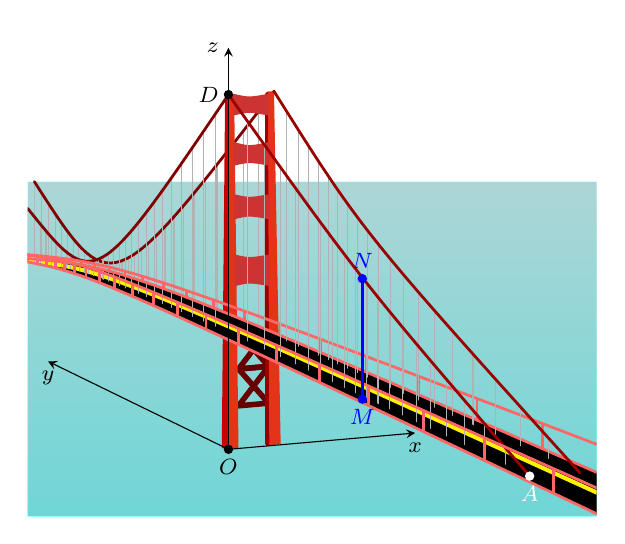
\begin{tikzpicture}[
					 scale=0.85,
					font=\footnotesize, 
					 line join=round,
					line  cap=round,
					 >=stealth]
				\clip (-3,-1) rectangle  (5.5,6.3);
				 \fill[opacity=0.8,bottom color=cyan!50!white,top color=cyan!20!white]
					 (-3,-1) rectangle (5.5,4);
				\begin{scope}
					\clip (0.68,5.35)..  controls (-1.75,2.2).. (-2.9,4) --
						 (-2.9,2.85).. controls (-2,2.5).. (0.68,1.75) -- cycle;
					\foreach \i  in {1,2,...,30}{
						\path (0.68,5.35).. controls (-1.75,2.2).. (-2.9,4) 
						coordinate[pos=\i/30]  (x);
						\draw[gray!60!white]  (x) -- ++(-90:4);
					} 
				\end{scope}
				\draw[red!50!black,line width=1pt] 
					(0.68,5.35).. controls (-1.75,2.2).. (-2.9,4); 
				\draw[line width=2pt,red!40!black] 
					(0.15,0.65) --  (0.6,0.69) -- (0.15,1.2) -- (0.6,1.24) -- cycle;
				\draw[line width=2pt,red!40!black,shift={(0,0.55)}] 
					(0.15,0.65) -- (0.6,0.69) -- (0.15,1.2) -- (0.6,1.24)  -- cycle;
				\node[brown!40!red,rotate=90] at (0.66,0.5) {1112}; 
				\draw[red!60!black,line width=2pt] (0.59,0.09) --  (0.59,5.3);
				\fill[brown!40!red] 
					(0.61,0.06) -- (0.59,5.35) -- (0.68,5.35) -- (0.78,0.08)  -- cycle;
				\fill[brown!40!red] 
					(0,0) coordinate (O) --  (0,5.3) coordinate (D) --
					(0.085,5.3) -- (0.15,0.02)  -- cycle;
				\fill[black!20!red] 
					(O) -- (D) -- (-0.05,5.32) -- (-0.1,0.02)  -- cycle;
				\fill[brown!60!red,draw,gray!40!red,line  width=0.5pt]
					(0.08,5.3).. controls (0.305,5.25).. (0.59,5.3)  --
					(0.591,5).. controls (0.305,5.05).. (0.084,5) --  cycle;
				 \fill[brown!60!red,draw,gray!40!red,line width=0.5pt]
					(0.085,4.58).. controls (0.306,4.52).. (0.603,4.58)  --
					(0.603,4.25).. controls  (0.3065,4.3).. (0.086,4.25) -- cycle;
				\fill[brown!60!red,draw,gray!40!red,line width=0.5pt] 
					 (0.091,3.8).. controls (0.307,3.75).. (0.605,3.8) --
					(0.606,3.45).. controls (0.307,3.5).. (0.093,3.45) --  cycle;
				\fill[brown!60!red,draw,gray!40!red,line  width=0.5pt]
					(0.098,2.9).. controls (0.308,2.85).. (0.608,2.9) -- 
					(0.609,2.45).. controls (0.308,2.5).. (0.099,2.45) -- cycle; 
				\fill (6,-1.2)..  controls (-2,2.6).. (-3,2.8) --
					(-3,2.85).. controls (-1.5,2.72).. (7,-1) -- cycle; 
				\draw[yellow,line  width=1.5pt]
					(6.5,-1.1).. controls (-1.75,2.66)..  (-3,2.825);
				\def\ipos{20} 
				\begin{scope}
					\clip  (0,5.3).. controls (-2,2.35).. (-3,3.6) --
						(-3,2.8)..  controls (-2.2,2.7).. (0,1.75) -- cycle;
					\foreach \i  in {1,2,...,30}{
						\path (0,5.3).. controls (-2,2.35)..  (-3,3.6)
						coordinate[pos=\i/30] (y); 
						 \draw[gray!60!white] (y) -- ++(-90:4);
					} 
				\end{scope}
				 \draw[red!50!black,line width=1pt]
					(0,5.3).. controls (-2,2.35).. (-3,3.6); 
				\draw[line width=1pt,red!60!white] 
					(7,-1).. controls (-1.5,2.72)..  (-3,2.85);
				\draw[line width=1pt,red!60!white] 
					(7,-0.5).. controls (-1.5,2.76).. (-3,2.91); 
				 \foreach \t in {1,2,...,\ipos}{
					\path (7,-1) coordinate  (c).. controls (-1.5,2.72).. (-3,2.85)
					coordinate[pos=\t/\ipos] (d); 
					\path (7,-0.5) coordinate (c')..  controls (-1.5,2.76).. (-3,2.91)
					coordinate[pos=\t/\ipos] (d'); 
					\draw[line width=1pt,red!60!white]  (d) -- (d');
				 }
				\begin{scope}
					\clip (D).. controls (2,2.5).. (4.5,-0.4) -- (0,1.75) -- cycle; 
					\foreach \i in {1,2,...,20}{ 
						\path (D).. controls (2,2.5)..  (4.5,-0.4)
						coordinate[pos=\i/20] (x'); 
						 \draw[gray!60!white] (x') -- ++(-90:4);
					 }
				\end{scope}
				\begin{scope}
					 \clip (0.68,5.35).. controls (2,3.25).. (5.25,-0.35) --
						(0.68,1.7)  -- cycle;
					\foreach \i in {1,2,...,20}{ 
						\path (0.68,5.35).. controls (2,3.25).. (5.25,-0.35) 
						coordinate[pos=\i/20]  (y');
						\draw[gray!60!white]  (y') -- ++(-90:4);
					 }
				\end{scope}
				\draw[red!60!black,line  width=1pt]
					(D)..  controls (2,2.5).. (4.5,-0.4);
				\draw[red!60!black,line width=1pt] 
					(0.68,5.35)..  controls (2,3.25).. (5.25,-0.35);
				\draw[line  width=1pt,red!60!white]
					(6,-1.2)..  controls (-2,2.6).. (-3,2.8);
				 \draw[line width=1pt,red!60!white]
					(6,-0.8).. controls (-2,2.78)..  (-3,2.9);
				\foreach \t  in {1,2,...,\ipos}{
					\path (6,-1.2) coordinate (a).. controls (-2,2.6).. (-3,2.8) 
					coordinate[pos=\t/\ipos] (b); 
					\path (6,-0.8) coordinate (a')..  controls (-2,2.78).. (-3,2.9)
					coordinate[pos=\t/\ipos] (b'); 
					\draw[line  width=1pt,red!60!white] (b) -- (b');
				} 
				\fill[white]  (4.5,-0.4) coordinate (A) node[below] {$A$} circle (2pt);
				\fill[blue] (2,0.75) coordinate (M) node[below] {$M$}  circle (2pt);
				\fill[blue] (2,2.55) coordinate (N) node[above] {$N$} circle (2pt); 
				\draw[blue,line  width=1pt] (M) -- (N);
				\draw[->] (O) -- (154:3)  node[below] {$y$};
				\draw[->] (O) --  (5:2.8) node[below] {$x$};
				\draw[->] (O) --  (90:6) node[left] {$z$};
				\fill (O) node[below]  {$O$} circle (2pt);
				\fill (D) node[left] {$D$}  circle (2pt);
			\end{tikzpicture}
	\end{center}
	\begin{center}
		 (\textit{Nguồn ảnh:} \href{https://www.goldengate.org/assets/1/6/ggb-exhibit-chapter-statistics.pdf}{https://www.goldengate.org/assets/1/6/ggb-exhibit-chapter-statistics.pdf})
	\end{center}
	Tính độ dài $MN$, biết điểm $M$ cách trục $Oz$ một khoảng bằng $230\ \text{ m}$ (Kết quả  làm tròn đến chữ số thập phân thứ hai sau dấu phẩy)
	 \shortans{50,1}
	 \loigiai{
		Ta có $A \in Oyz$ và $A$ cách mặt nước $75\ \text{  m}$ và cách trục $Oz\ 343\ \text{ m} \Rightarrow A(0;343;75)$
		\noindent Điểm $D$ là đỉnh cột trụ cách mặt  nước $227\ \text{ m} \Rightarrow D(0;0;227) \Rightarrow \vec{AD} = (0;-343;152)$
		\noindent Phương trình  đường thẳng $AD$ là
		 \[
		\begin{cases}
			x =  0 \\
			y = -343t  \\
			z = 227  + 152t
		\end{cases}\quad (t \in \mathbb{R})
		\] 
		\noindent Vì $N \in AD \Rightarrow N\left(0;-343t;227 + 152t\right)$ 
		\noindent Điểm $M$ trên thành cầu, $M$ cách mặt nước $75\ \text{ m}$ và cách trục $Oz$ một khoảng $230\ \text{ m}$  nên toạ độ điểm $M$ là $M(0;230;75)$
		\noindent $\Rightarrow \vec{MN} = \left(0;-343t - 230;152  + 152t\right)$
		\noindent $MN$ song song với  cột trụ $\Rightarrow \vec{MN} \perp Oy \Rightarrow \vec{MN} \cdot \vec{j} = 0 \Rightarrow -343t - 230 = 0 \Leftrightarrow t = -\dfrac{230}{343}$.
		\noindent $\Rightarrow \vec{MN} = \left(0;0;\dfrac{17176}{343}\right) \Rightarrow  MN = \dfrac{17176}{343} \approx 50,08\ \text{ m}$.
	} 
\end{bt}

% nguồn: Phan2_Lop_12_Hinh_hoc_Chuong_5
\begin{bt}%[2H5H2-8]%[ma:c9b5338a]
	Trong không gian $Oxyz$, một cabin cáp treo xuất phát từ điểm $A(-2;1;5)$ và chuyển động đều theo đường cáp có vectơ chỉ phương là $\vec{u}=(0;-2;6)$ với tốc độ là $4$ m/s (đơn vị trên mỗi trục toạ độ là mét). Giả sử sau $5$ (s) kể từ lúc xuất phát, cabin đến  điểm $M$. Gọi tọa độ $M(a;b;c)$. Tính $2a+3b+c$.
	\shortans{4} 
	\loigiai{Gọi $t$ là thời gian cabin di chuyển, sau $5$  (s) kể từ lúc xuất phát, cabin đến điểm $M$ thì $$AM=4\cdot 5=20~\text{ (m)}.$$
		Gọi $d$ là đường di chuyển của cabin,  ta có $$d\colon \heva{&\text{ đi qua }A(-2;1;5)\\&\text{ có vectơ chỉ phương }\vec{u}=(0;-2;6)}\Rightarrow d\colon \heva{&x=-2\\&y=1-2t\\&z=5+6t.}$$
		Vì $M \in d \Rightarrow M(-2;1-2t;5+6t)\Rightarrow\vec{AM}=(0;-2t;6t)$.\\ Do  $2$ vectơ $\vec{A M}$; $\vec{u}$ cùng hướng nên $t>0$.\\Ta có
		\allowdisplaybreaks 
		\begin{eqnarray*}
			A M&=&20 \Leftrightarrow \sqrt{0^2+4 t^2+36 t^2}=20 \Leftrightarrow 40  t^2=400 \Leftrightarrow t= \pm \sqrt{10}.
		\end{eqnarray*}
		Vì $t>0 \Rightarrow  t=\sqrt{10}$.\\
		Vậy  tọa độ $M\left( -2;1-2\sqrt{10}; 5+6\sqrt{10}\right)$. \\Khi đó $2 a+3 b+c=-4+3\left(1-2 \sqrt{10}\right)+5+6 \sqrt{10}=4$.
	} 
\end{bt}

% nguồn: Phan2_Lop_12_Hinh_hoc_Chuong_5
\begin{bt}%[2H5H2-8]%[ma:d2c71fc6]
	Trong một khu du lịch, người ta cho du khách trải nghiệm thiên nhiên bằng cách đu theo đường trượt zipline từ vị trí $A$ cao $15$ m của tháp $1$ này sang vị trí $B$ cao $10$ m của tháp $2$ trong khung cảnh tuyệt đẹp xung quanh. Với  hệ trục toạ độ $Oxyz$ cho trước (mét), tọa độ của $A$ và $B$ lần lượt là $(3;2{,}5;15)$ và $(21;27{,}5;10)$. Khi du khách khi ở độ cao $12$ m thì toạ độ khi đó là $M(a;b;c)$. Tính giá trị biểu thức $T=a+b+c$. (Kết quả làm tròn đến hàng phần chục).
	\shortans{37,3} 
	 \loigiai{
		Ta có: $\vec{AB}=(18;15;-5)$.\\ 
		 Phương trình tham số đường thẳng $AB$ là $\heva{&x=3+18t\\&y=2{,}5+15t\\&z=15-5t\quad(t\in\mathbb{R})}$.\\
		Khi  du khách ở độ cao $12$ m $\Rightarrow z=12 \Rightarrow 15-5t=12 \Rightarrow t=\dfrac{3}{5}$.\\
		Thay $t=\dfrac{3}{5}$ vào ta được $M(13{,}8;11{,}5;12) \Rightarrow T = 13{,}8 + 11{,}5 + 12 = 37{,}3$. 
	 }
\end{bt}

% nguồn: Phan2_Lop_12_Hinh_hoc_Chuong_5
\begin{bt}%[2H5H2-8]%[ma:d05886a0]
	Trong không gian với hệ trục tọa độ $Oxyz$, với mặt phẳng $(Oxy)$ là mặt đất, một máy bay cất cánh từ vị trí $A(0; 10; 0)$ với vận tốc $\vec{v}=(150; 150; 40)$. Biết góc nâng của máy bay là $\gamma=a^\circ$ (góc giữa hướng chuyển động bay lên của máy bay với đường băng và làm tròn  kết quả đến hàng độ). Khi đó giá trị của $a$ bằng bao nhiêu?
	 \shortans{11}
	 \loigiai{
		Phương trình đường thẳng chuyển động của máy bay là $d\colon \heva{& x=150t\\& y=10+150t\\ & z=40t}$ với $t\ge 0$ tính theo đơn  vị giây là thời gian chuyển động của máy bay.\\
		Sau $t=1$  giây thì máy bay bay tới vị trí $B(150;160;40)$.\\
		Gọi $C$ là hình chiếu vuông góc của máy  bay sau $1$ giây lên trên mặt đất, suy ra $C(150;160;0)$ và $BC=40$, $AC=150\sqrt{2}$.\\
		Khi đó, góc  giữa hướng chuyển động bay lên của máy bay với đường băng là $\gamma=\widehat{BAC}$.\\
		Xét $\triangle ABC$ có $\tan \widehat{BAC}=\dfrac{BC}{AC}=\dfrac{40}{150\sqrt{2}}$.\\ 
		Suy ra $\gamma=\widehat{BAC}\approx 11^\circ$, do đó  $a=11$.
	} 
\end{bt}

% nguồn: Phan2_Lop_12_Hinh_hoc_Chuong_5
\begin{bt}%[2H5H2-8]%[ma:a8be6b8f]
	Trong không gian $Oxyz$, đài kiểm soát không lưu  sân bay có tọa độ $O (0; 0; 0)$, đơn vị trên mỗi trục tính theo kilômét. Một máy bay chuyển động hướng về dài kiểm soát không lưu, bay qua hai vị trí $A \left(-500; -250; 150\right)$, $B \left(-200; -200; 100\right)$. Khi máy bay ở gần đài kiểm soát nhất, tọa độ của vị trí máy bay là $\left(a; b; c\right)$. Giá trị của biểu thức $-3a - b -c$ là bao nhiêu (làm tròn kết quả đến hàng đơn vị)?
	\shortans{-11} 
	\loigiai{ 
		Ta có $\overrightarrow{AB}  = \left(300; 50; -50\right)$. \\
		Vậy vectơ $\vec{u} = \left(6; 1;  -1\right)$ là một vectơ chỉ phương của đường thẳng $AB$. \\
		Phương trình tham số của đường thẳng $AB$ là $\heva{&  x = -500 +6t \\ & y = -250 +t \\ & z = 150 -t}$ với $t \in \mathbb{R}$. \\
		Gọi $H$ là hình chiếu của điểm $O$ lên  đường thẳng $AB$. Khi đó $OH$ chính là khoảng cách ngắn nhất từ máy bay đến đài kiểm soát không lưu. \\
		Do  $H \in AB \Rightarrow H \left(-500+6t; -250 +t; 150 -t \right)$ với $t \in \mathbb{R}$. \\
		 Khi đó $\overrightarrow{OH} = \left(-500+6t; -250 +t; 150 -t \right)$. \\
		Do $OH \perp AB$ nên $\overrightarrow{OH} \cdot \vec{u} =0 \Leftrightarrow (6t-500) \cdot 6 + \left(t-250 \right)  + \left(t -150 \right) = 0 \Leftrightarrow t = \dfrac{1700}{19}$. \\
		Suy  ra vị trí của máy bay khi đó là $\left(\dfrac{700}{19}; - \dfrac{3050}{19}; \dfrac{1150}{19}\right)$. \\
		Vậy, ta có kết quả $-3 a - b - c = -3 \cdot \dfrac{700}{19} + \dfrac{3050}{19} - \dfrac{1150}{19} =  - \dfrac{200}{19} \approx -11$.
	} 
\end{bt}

% nguồn: Phan2_Lop_12_Hinh_hoc_Chuong_5
\begin{bt}%[2H5H2-8]%[ma:d71579f0]
	Một máy bay cất cánh tại một sân bay, sau khi bắt đầu cất cánh trong thời gian ngắn, máy bay sẽ bay theo một đường thẳng và sân bay nơi máy bay cất cánh được coi là một mặt phẳng. Chọn hệ tọa độ $Oxyz$ (\textit{đơn vị đo tính bằng km}). Biết rằng, máy bay bắt đầu cất cánh tại điểm $O(0;0;0)$ và sau một thời gian ngắn, máy bay bay đến điểm $A(2;\,5;\,1{,}2)$, sân bay nơi máy bay cất cánh nằm trên mặt phẳng $(Oxy)$. Hỏi góc tạo bởi đường bay của máy bay  khi cất cánh và sân bay bằng bao nhiêu (\textit{làm tròn kết quả đến hàng đơn vị, tính theo độ})?
	\shortans{13} 
	 \loigiai{
		Dựa vào đề bài, ta thấy góc tạo bởi đường bay của máy bay cất cánh và sân bay  chính là góc giữa $\overrightarrow{OA}$ và mặt phẳng $(Oxy)$.\\
		Ta có $\overrightarrow{OA} = (2;\,5;\,1{,}2)$ và vectơ pháp tuyến của mặt phẳng $(Oxy)$  là $\vec{n}= (0;0;1)$.\\
		Gọi $\alpha$ là  góc tạo bởi $\overrightarrow{OA}$ và mặt phẳng $(Oxy)$, ta có
		\begin{align*}
			\sin\alpha  = \dfrac{\left| \overrightarrow{OA}\cdot\vec{k}\right| }{\left|\overrightarrow{OA}\right|\cdot\left|\vec{k}\right|}
			= \dfrac{\left|1{,}2\right|}{\sqrt{2^2 + 5^2 + (1{,}2)^2}\cdot1} 
			 = \dfrac{6\sqrt{761}}{761}.
		\end{align*}
		Suy  ra $\alpha \approx 13^\circ$.
	 }
\end{bt}

% nguồn: Phan2_Lop_12_Hinh_hoc_Chuong_5
\begin{bt}%[2H5H2-8]%[ma:69e7c8dc]
	Khi gắn  hệ tọa độ $Oxyz$ (đơn vị trên mỗi trục tính theo kilômét) vào một sân bay, mặt phẳng $(Oxy)$ trùng với mặt sân bay. Một máy bay bay theo đường thẳng từ vị trí $A(3;-2;3)$ đến vị trí $B(5;6;2)$. Góc giữa đường bay (một phần của đường thẳng $AB$) và sân bay (một phần của mặt phẳng($Oxy$)) bằng $a$ độ (làm tròn kết quả đến hàng đơn vị). Tính giá trị của $a$.
	\shortans{7} 
	 \loigiai{
		Gọi $\alpha$ là góc tạo bởi mặt phẳng $(Oxy)$ (có  một vectơ pháp tuyến $\vec{k}=(0;0;1)$) và $\vec{AB} = (2;8;-1)$ thì
		 $$
		 \sin\alpha
		= \dfrac{|\vec{AB}  \cdot \vec{k}|}{|\vec{AB}| \cdot |\vec{k}|}
		 = \dfrac{|-1|}{\sqrt{69} \cdot 1}
		=  \dfrac{1}{\sqrt{69}}.
		 $$
		Suy ra $\alpha = 7^\circ$ và $a = 7$. 
	 }
\end{bt}

% nguồn: Phan2_Lop_12_Hinh_hoc_Chuong_5
\begin{bt}%[2H5H2-8]%[ma:b6f73017]
	Trong không gian $Oxyz$, một viên đạn được bắn ra từ điểm $A(1; 2; 3)$ và trong $3$ giây, đầu đạn đi với vận tốc  không đổi; vectơ vận tốc (trên giây) là $\vec{v} = (2; 1; 5)$. Khi viên đạn trúng mục tiêu tại điểm $B(-5; a; b)$ thì giá trị của biểu thức $b^a$ bằng bao nhiêu? (kết quả làm tròn đến hàng phần chục).
	\shortans{-0,1} 
	 \loigiai{
		Phương trình mô tả quỹ đạo chuyển động của viên đạn là $\heva{& x=1+2t \\  & y=2+t \\ & z=3+5t} \ (1)$.\\
		Khi viên đạn trúng mục tiêu tại điểm $B(-5; a; b)$ thì tọa độ của điểm $B$ thỏa $(1)$, tức là $$\heva{& -5=1+2t \\ & a=2+t \\ & b=3+5t} \Leftrightarrow  \heva{& t=-3 \\ & a=2+t \\ & b=3+5t} \Leftrightarrow \heva{& t=-3 \\ & a=-1 \\ & b=-12 } \Rightarrow b^a \approx -0{,}1.$$
	} 
\end{bt}

% nguồn: Phan2_Lop_12_Hinh_hoc_Chuong_5
\begin{bt}%[2H5V2-8]%[ma:300b3e0e]
	Trong một đợt diễn tập quốc phòng, hai người ở vị trí khác nhau cùng ngắm bắn một mục tiêu cố định trên không. Người ta gắn một hệ trục tọa độ $Oxyz$ (đơn vị trên mỗi trục tính theo mét), mặt phẳng $(Oxy)$ trùng với mặt đất. Người thứ nhất bắn một viên đạn đi qua hai điểm $A(5;7;10)$ và $B(6;9;12)$. Người thứ hai bắn một viên đạn đi qua  hai điểm $C(15;17;5)$ và $D$ (điểm $D$ ở độ cao $26$m so với mặt đất). Biết rằng sau một thời gian rời khỏi nòng súng, hai viên đạn chạm với nhau tại vị trí cách điểm $A$ một khoảng $150$m (tham khảo hình vẽ)
	\begin{center}
		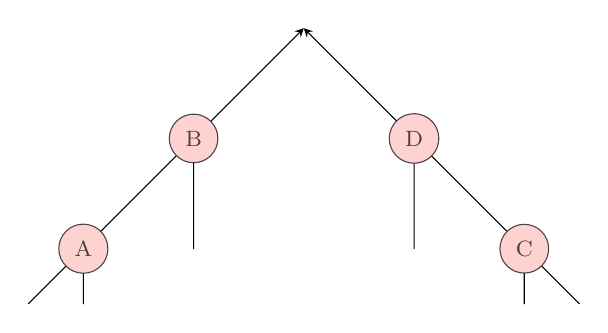
\begin{tikzpicture}[scale=0.7,>=stealth,x=1cm,y=1cm,font=\footnotesize,line join=round,line cap=round]
				\node[circle,fill=pink,opacity=0.7,draw]  (A) at (-4,1){A};
				\node[circle,fill=pink,opacity=0.7,draw] (B) at  (-2,3){B};
				\node[circle,fill=pink,opacity=0.7,draw] (C)  at (4,1){C};
				\node[circle,fill=pink,opacity=0.7,draw] (D) at  (2,3){D};
				 \draw[->] (-5,0)--(A)--(B)--(0,5);
				\draw[->] (5,0)--(C)--(D)--(0,5); 
				 \draw (-4,0)--(A)
					 (-2,1)--(B)
					 (4,0)--(C)
					 (2,1)--(D);
			\end{tikzpicture}
	\end{center}
	Hỏi  điểm $D$ cách điểm $C$ một khoảng bao nhiêu mét? (Kết quả làm tròn đến hàng phần chục)
	\shortans{28,8} 
	 \loigiai{
		Gọi $E\left( x;\,y;\,z \right)$ là  điểm va chạm của hai viên đạn.\\
		Ta có: $\overrightarrow{AB}=\left(  1;\,2;\,2 \right)\Rightarrow AB=\sqrt{1^{2}+2^{2}+2^{2}}=3$.\\
		Theo bài ra, ta có: $AE=150\,$; $\overrightarrow{AB}$ và  $\overrightarrow{AE}$ cùng hướng.\\
		Do đó:  $\overrightarrow{AE}=\dfrac{150}{3}\overrightarrow{AB}\Leftrightarrow \heva{
		x-5=50\cdot 1  \\
		 y-7=50\cdot 2 \\
		z-10=50 \cdot 2 }  \Leftrightarrow \heva{
		x=55  \\
		y=107  \\
		z=110}$  $\Rightarrow E\left( 55;\,107;\,110 \right).$\\
		Ta có: $\overrightarrow{CE}=\left( 40;\,90;105 \right)$ $\Rightarrow \vec{u}=\left( 8;\,18;21 \right)$  là vectơ chỉ phương của đường thẳng $CE$.\\
		Phương trình đường thẳng $CE$ là: $\heva{ 
		x=15+8t  \\
		 y=17+18t \\
		z=5+21t  }.$\\
		Theo bài ra  ta có: $D\left( a;\,b;\,26 \right)\in CE$ nên: $\heva{
		a=15+8t \\ 
		 b=17+18t \\
		 26=5+21t} \Leftrightarrow \heva{
		a=23 \\ 
		 b=35 \\
		t=1 }  \Rightarrow D\left( 23;\,35;\,26 \right).$\\
		Vậy $CD=\sqrt{\left( 23-15 \right)^{2}+\left( 35-17 \right)^{2}+\left( 26-5  \right)^{2}}=\sqrt{829}\approx 28{,}8.$
	} 
\end{bt}

% nguồn: Phan2_Lop_12_Hinh_hoc_Chuong_5
\begin{bt}%[2H5V2-8]%[ma:eacb9231]
	Cầu Cổng Vàng (The Golden Gate Bridge) ở Mỹ. Xét hệ trục toạ độ $Oxyz$ với $O$ là bệ của chân cột trụ tại mặt nước, trục $Oz$ trùng với cột trụ, mặt phẳng ($Oxy$) là mặt nước và xem như trục $Oy$ cùng  phương với cầu như hình vẽ. Dây cáp $AD$ (xem như là một đoạn thẳng) đi qua đỉnh $D$ thuộc trục $Oz$ và điểm $A$ thuộc mặt phẳng ($Oyz$), trong đó điểm $D$ là đỉnh cột trụ cách mặt nước $326$ m, điểm $A$ cách mặt nước $82$ m và cách trục $Oz$ khoảng $352$ m.
	\begin{center}
		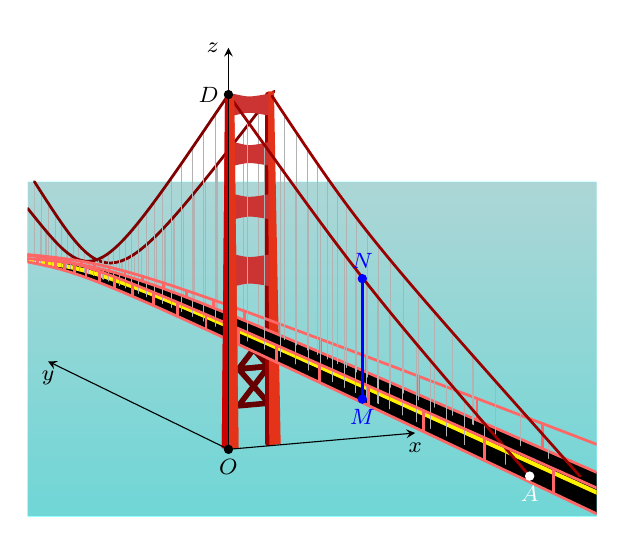
\begin{tikzpicture}[scale=0.85,font=\footnotesize,line join=round,line cap=round,>=stealth]
				\clip (-3,-1) rectangle (5.5,6.3); 
				\fill[opacity=0.8,bottom  color= cyan!50!white,top color= cyan!20!white] (-3,-1) rectangle (5.5,4);
				\begin{scope}
					 \clip (0.68,5.35).. controls (-1.75,2.2).. (-2.9,4) -- (-2.9,2.85).. controls (-2,2.5).. (0.68,1.75) -- (0.68,5.35);
					 \foreach \i in {1,2,...,30}
						{\path 
						(0.68,5.35).. controls (-1.75,2.2).. (-2.9,4)  coordinate[pos=\i/30](x);
					 \draw[gray!60!white] (x)--++(-90:4);}
				\end{scope}
				\draw[red!50!black,line width=1pt]  ((0.68,5.35).. controls (-1.75,2.2).. (-2.9,4);
				\draw[line width =2pt,red!40!black] (0.15,0.65) -- (0.6,0.69) -- (0.15,1.2) -- (0.6,1.24) --  cycle;
				\draw[line width =2pt,red!40!black,shift={(0,0.55)}] (0.15,0.65)  -- (0.6,0.69) -- (0.15,1.2) -- (0.6,1.24) -- cycle;
				\draw[red!60!black,line width=2pt] (0.59,0.09) -- (0.59,5.3); 
				 \fill[brown!40!red]
					(0.61,0.06) -- (0.59,5.35) -- (0.68,5.35)  -- (0.78,0.08) -- cycle;
				\fill[brown!40!red] (0,0) coordinate (O) -- (0,5.3) coordinate (D) -- (0.085,5.3)  -- (0.15,0.02) -- cycle;
				 \fill[black!20!red]
					(O) -- (D) -- (-0.05,5.32) --  (-0.1,0.02) -- cycle;
				\fill[brown!60!red,draw,gray!40!red,line width=0.5pt] (0.08,5.3).. controls (0.305,5.25).. (0.59,5.3)  -- (0.591,5).. controls (0.305,5.05)..(0.084,5) -- cycle;
				\fill[brown!60!red,draw,gray!40!red,line width=0.5pt] (0.085,4.58).. controls (0.306,4.52).. (0.603,4.58) -- (0.603,4.25).. controls  (0.3065,4.3)..(0.086,4.25) -- cycle;
				\fill[brown!60!red,draw,gray!40!red,line width=0.5pt] (0.091,3.8)..  controls (0.307,3.75).. (0.605,3.8) -- (0.606,3.45).. controls (0.307,3.5)..(0.093,3.45) -- cycle;
				\fill[brown!60!red,draw,gray!40!red,line width=0.5pt] (0.098,2.9).. controls  (0.308,2.85).. (0.608,2.9) -- (0.609,2.45).. controls (0.308,2.5)..(0.099,2.45) -- cycle;
				\fill (6,-1.2).. controls  (-2,2.6).. (-3,2.8) -- (-3,2.85).. controls (-1.5,2.72).. (7,-1)--cycle;
				\draw[yellow,line width = 1.5pt] (6.5,-1.1).. controls  (-1.75,2.66).. (-3,2.825);
				 \def\ipos{20}
				\begin{scope}
					\clip (0,5.3).. controls  (-2,2.35).. (-3,3.6) -- (-3,2.8).. controls (-2.2,2.7).. (0,1.75) -- cycle;
					 \foreach \i in {1,2,...,30}
						 {\path
						(0,5.3).. controls (-2,2.35).. (-3,3.6) coordinate[pos=\i/30](y); 
					\draw[gray!60!white] (y)--++(-90:4);} 
				\end{scope}
				\draw[red!50!black,line width=1pt] 
					 (0,5.3).. controls (-2,2.35).. (-3,3.6);
				\draw[line width=1pt,red!60!white] (7,-1).. controls (-1.5,2.72)..  (-3,2.85)
					(7,-0.5)..  controls (-1.5,2.76).. (-3,2.91);
				\foreach  \t in {1,2,...,\ipos}
					{\path 
					(7,-1) coordinate (c).. controls (-1.5,2.72).. (-3,2.85)  coordinate[pos=\t/\ipos](d)
					(7,-0.5) coordinate (c').. controls (-1.5,2.76)..  (-3,2.91) coordinate[pos=\t/\ipos](d');
				\draw[line width=1pt,red!60!white]  (d)--(d');}
				\begin{scope}
					\clip  (D).. controls (2,2.5).. (4.5,-0.4) -- (0,1.75) --cycle;
					\foreach  \i in {1,2,...,20}
						 {\path
						 (D).. controls (2,2.5).. (4.5,-0.4) coordinate[pos=\i/20](x');
					\draw[gray!60!white]  (x')--++(-90:4);}
				\end{scope}
				\begin{scope}
					 \clip (0.68,5.3).. controls (2,3.25).. (5.25,-0.35) -- (0.69,1.7) --cycle;
					\foreach \i in  {1,2,...,20}
						 {\path
						(0.65,5.28)..  controls (2,3.25).. (5.25,-0.4) coordinate[pos=\i/20](y');
					\draw[gray!60!white]  (y')--++(-90:4);}
				\end{scope}
				 \draw[red!60!black,line width=1pt] (D).. controls (2,2.5).. (4.5,-0.4)
					(0.65,5.28).. controls  (2,3.25).. (5.25,-0.4);
				\draw[line width=1pt,red!60!white] (6,-1.2).. controls  (-2,2.6).. (-3,2.8)
					(6,-0.8).. controls (-2,2.78).. (-3,2.9); 
				 \foreach \t in {1,2,...,\ipos}
					{\path (6,-1.2)  coordinate (a).. controls (-2,2.6).. (-3,2.8) coordinate[pos=\t/\ipos](b)
					 (6,-0.8) coordinate (a').. controls (-2,2.78).. (-3,2.9) coordinate[pos=\t/\ipos](b');
				\draw[line width=1pt,red!60!white] (b)--(b');} 
				\fill[brown!40!red] (0,0) -- (0,5.3)  -- (0.085,5.3) -- (0.15,0.02) -- cycle;
				\fill[black!20!red] 
					(O) -- (D) -- (-0.05,5.32)  -- (-0.1,0.02) -- cycle;
				\fill[white] (4.5,-0.4) coordinate (A) node[below]{$A$} circle (2pt); 
				\fill[blue]  (2,0.75) coordinate (M) node[below]{$M$} circle (2pt);
				 \fill[blue] (2,2.55) coordinate (N) node[above]{$N$} circle (2pt);
				 \draw[blue,line width=1pt] (M)--(N);
				\draw[->]  (O) -- (154:3) node[below]{$y$};
				 \draw[->] (O) -- (5:2.8) node[below]{$x$};
				\draw[->] (O) -- (90:6)  node[left]{$z$};
				\fill (O)  node[below]{$O$} circle (2pt)
					(D) node[left]{$D$} circle (2pt); 
			\end{tikzpicture}
	\end{center}
	Giả sử ta dùng một đoạn dây nối điểm $N$ trên dây cáp $AD$ và điểm $M$ trên thành cầu, biết $M$ cách mặt nước $82$ m và $MN$  song song với cột trụ. Tính độ dài đoạn $MN$, biết điểm $M$ cách trục $Oz$ một khoảng bằng $250$ m (Kết quả làm tròn đến hàng đơn phần chục).
	\shortans{70,7} 
	\loigiai{ 
		Ta có $A \in (Oyz)$ và $A$ cách mặt nước $82$ m và cách trục $Oz$ một  khoảng $352$ m nên $A(0;352;82)$.\\
		Điểm $D$ là đỉnh cột trụ cách mặt nước $326$ m  nên $D(0;0;326) \Rightarrow \overrightarrow{AD} = (0;-352;244)$.\\
		Phương trình  đường thẳng $AD$ là
		$$\begin{cases} x = 0 \\ y = -352t \\ z = 326 + 244t
	\end{cases} \quad (t \in \mathbb{R}).$$
	Vì $N \in AD \Rightarrow N(0;-352t;326+244t)$.\\ 
	Điểm $M$ trên thành cầu,  $M$ cách mặt nước $82$ m và cách trục $Oz$ một khoảng bằng $250$ m nên tọa
	độ điểm $M$  là $M(0;250;82)$.\\
	Nên $\overrightarrow{MN} =  (0;-352t-250;244+244t)$.\\
	Ta có $MN$ song song với cột trụ nên $MN \perp Oy$ hay $$ \overrightarrow{MN}\cdot \overrightarrow{j} = 0 \Rightarrow  -352t-250 = 0 \Leftrightarrow t = -\dfrac{125}{176}.$$
Suy ra $\overrightarrow{MN} = \left(0;0;\dfrac{3\,111}{44}\right)  $ nên $MN = \dfrac{3\,111}{44} \approx 70{,}7$ m.}
\end{bt}

% nguồn: Phan2_Lop_12_Hinh_hoc_Chuong_5
\begin{bt}%[2H5V2-8]%[ma:f21295bd]
	Trong không gian với hệ trục tọa độ $Oxyz$, xét mô hình phòng không như sau: radar đặt tại gốc tọa độ $O\left(0;0;0\right)$, tên lửa phòng không đặt tại điểm $M\left(0;50;0\right)$, mỗi đơn vị tương ứng với $10$ (m), mặt phẳng $\left(Oxy\right)$ trùng với mặt đất, trục $Oz$ vuông góc với mặt đất và  hướng lên. Giả sử mọi UAV (phương tiện bay không người lái) và tên lửa đều chuyển động thẳng đều. Tại thời điểm $t=0$ (s), radar phát hiện ra UAV $A$ ở tọa độ $A_0\left(1\,100;0;15\right)$.
	Tại thời điểm $t=1$ (s), radar theo dõi thấy UAV $A$ ở tọa độ $A_1\left(1\,095;1;14{,}5\right)$ trên đường thẳng $d$. Tại thời điểm $t=6$ (s),  một tên lửa được phóng lên và chuyển động thẳng đều với vận tốc $1\,300$ (m/s), va chạm và phá hủy UAV $A$ tại điểm $B$ trên $d$. Hỏi sau bao nhiêu giây kể từ lúc được phóng lên thì tên lửa va chạm với UAV $A$ (làm tròn kết quả đến hàng phần trăm của giây)?
	\shortans{7,93} 
	 \loigiai{
		Ta có  $\overrightarrow{A_0A_1}=\left(-5;1;-0{,}5\right)$.\\
		Vị trí của UAV $A$ sau thời gian $t$  giây kể từ khi xuất phát là $\heva{
		& x=1\,100-5t\\ 
		 & y=t\\
		& z=15-0{,}5t.}$\\ 
		Do đó  $B\left(1\,100-5t_1;{t_1};15-0{,}5t_1\right)$.
		\begin{eqnarray*}
			 &MB&=\left|\overrightarrow{MB}\right|\\
			&&=\sqrt{\left(1\,100-5t_1\right)^2+\left(t_1-50\right)^2+\left(15-0{,}5t_1\right)^2}\\ 
			&&=\sqrt{26{,}25t_1^2-11\,115t_1+1\,212\,725}. 
		\end{eqnarray*}
		Tại thời điểm $t=6$ thì tên lửa được phóng lên nên thời gian từ lúc tên lửa được phóng  lên đến lúc va chạm với UAV $A$ là $t_1-6$ (s).\\
		Do mỗi đơn vị tương ứng với $10$ (m) nên độ dài quãng  đường $MB$ là $$10\sqrt{26{,}25t_1^2-11\,115t_1+1\,212\,725}\text{ (m).}$$
		Ta có phương trình  $10\cdot\sqrt{26{,}25t_1^2-11\,115t_1+1\,212\,725}=1\,300\cdot\left(t_1-6\right)$.\\
		Giải phương trình  trên thu được $t_1\approx 13{,}93$.\\
	Thời gian kể từ lúc tên lửa được phóng lên đến lúc va  chạm với UAV $A$ là $t_1-6\approx 7{,}93$ (s).}
\end{bt}

% nguồn: Phan2_Lop_12_Hinh_hoc_Chuong_5
\begin{bt}%[2H5V2-8]%[ma:a3596a23]
	Quỹ đạo của một tia sáng được theo dõi. Tia  sáng xuất phát từ điểm $A(0;6;6)$ theo hướng của vectơ $\overrightarrow{v}=(1;-1;-2)$ và đi tới mặt phẳng $xOy$, tại đó nó bị phản xạ. Tia sáng phản xạ cắt mặt phẳng $xOz$ tại điểm $C(a;b;c)$. Tính $a+b+c$?
	\begin{center}
		\begin{tikzpicture}[line cap=round,line join=round,>=stealth,font=\footnotesize]
				 \tikzset{denpin/.pic={
				\begin{scope}[scale=0.5]
					 \def\a{1}
					 \draw (0,0)--++(60:\a) arc (-30:150:0.3)--++(-120:\a)--cycle;
					\draw[ball color=white] (0,0)++(150:0.3) coordinate  (A) circle (0.3);
					\draw[ball color=yellow] (A) circle (0.2); 
					\foreach  \x in{-2,-1,0,1,2}{\draw[yellow,line width=1pt] (A)--++({-120+10*\x}:1);}
				\end{scope}
					}} 
				\begin{scope}[scale=0.5]
					\fill[cyan!20] (0,0) rectangle  (8,8);
					\fill[orange!20] (0,0)--++(0:8)--++(-135:8)--++(180:8)  coordinate (H)--cycle;
					\fill[yellow!20]  (0,0)--(H)--++(90:8)--++(45:8)--cycle;
					\def\a{8} 
					 \pgfmathsetmacro{\b}{\a-1};
					\draw[->] (0,0)--++(0:\a)  node[below] {$y$};
					 \draw[->] (0,0)--++(-135:\a) node[right] {$x$};
					 \draw[->] (0,0)--++(90:\a) node[left] {$z$};
					 \foreach \x in{1,...,\b}{
						\draw (\x,0) node[below]  {$\x$}--++(90:\b);
						\draw  (0,\x) node[left] {$\x$} --++(0:\b);
						 \draw (\x,0)--++(-135:\b);
						\draw (0,\x)--++(-135:\b); 
						\draw  (0,0)++(-135:\x) node[below] {$\x$}--++(0:\b);
						 \draw (0,0)++(-135:\x)--++(90:\b);
					 }
					 \path
						(6,6) coordinate (A) 
						(0,0)++(0:3)++(-135:3) coordinate (B) 
						(0,0)++(90:6)++(-135:6) coordinate (C) 
						 ($(A)!0.3!(B)$) coordinate (A')
						 ($(A)!0.7!(B)$) coordinate (B')
						($(B)!0.3!(C)$)  coordinate (C')
						 ($(B)!0.7!(C)$) coordinate (D');
					 \draw[->,line width=2pt,blue] (A')--(B');
					 \draw[->,line width=2pt,blue] (C')--(D');
					\draw[line  width=1pt,red] (A)--(B)--(C);
					\foreach  \x/\y in{A/above right,B/above,C/above right}{\draw (\x) circle (2pt) node[\y] {$\x$};}
					\pic at  (7.5,7.5) {denpin};
				\end{scope}
			\end{tikzpicture}
	\end{center}
	 \shortans{12}
	 \loigiai{
		Tia sáng  là một đường thẳng $g$ đi qua điểm
		$A(0;6;6)$,  nhận $(1;-1;-2)$ làm vectơ chỉ phương nên có phương trình \[\heva{&x=0+t\\ &y=6-t\\ &z=6-2t.}\]
		Giao điểm của đường thẳng $g$ với mặt  phẳng $xOy\colon z=0$ là nghiệm của hệ phương trình \[\heva{&x=0+t\\ &y=6-t\\ &z=6-2t\\&z=0}\Leftrightarrow \heva{&t=3\\&x=3\\&y=3\\&z=0}\Rightarrow B(3;3;0).\]
		Tia phản xạ $h$ là một đường thẳng đi qua điểm $B(3;3;0)$, nhận $(1;-1;2)$ làm vectơ chỉ phương nên có phương trình \[\heva{&x=3+s\\  &y=3-s\\ &z=0+2s.}\]
		Giao điểm của đường thẳng $h$ với mặt phẳng $xOz$ là nghiệm của hệ phương trình \[\heva{&x=3+s\\  &y=3-s\\ &z=0+2s\\&y=0}\Leftrightarrow \heva{&s=3\\&x=6\\&y=0\\&z=6}\Rightarrow C(6;0;6).\]
		Vậy  $a+b+c=12$.
	} 
\end{bt}

% nguồn: Phan2_Lop_12_Hinh_hoc_Chuong_5
\begin{bt}%[2H5V2-8]%[ma:c3943bf2]
	Tại một nút giao thông có $2$ con đường khác mức. Trên thiết kế, trong  không gian $Oxyz$ hai con đường đó thuộc hai đường thẳng $d_1\colon \dfrac{x-2}{1}=\dfrac{y-2}{1}=\dfrac{z}{-1}$ và $d_2\colon \dfrac{x-2}{1}=\dfrac{y+1}{2}=\dfrac{z}{-3}$. \\
	Người ta muốn tạo một con đường $\Delta$ cắt $d_1$, $d_2$ lần lượt tại $A$  và $B$ sao cho $AB$ nhỏ nhất. Tính độ dài $AB$ (kết quả làm tròn đến hàng phần trăm).
	\shortans{2,45} 
	\loigiai{ 
		Ta có $AB$ ngắn nhất khi  $AB$ là đoạn vuông góc chung của $d_1$ và $d_2$.\\
		Gọi $A(2+a;2+a;-a) \in d_1$, $B(2+b;-1+2b;-3b)  \in d_2$. Suy ra $\overrightarrow{AB}=(b-a;2b-a-3;-3b+a)$.\\
		Ta thấy $d_1$, $d_2$  lần lượt có các vectơ chỉ phương là $\vec{u}_1=(1;1;-1)$ và $\vec{u}_2=(1;2;-3)$.\\
		 Lúc đó
		$$\heva{&\overrightarrow{AB} \cdot \vec{u}_1=0 \\& \overrightarrow{AB} \cdot \vec{u}_2=0} \Leftrightarrow\heva{&1(b-a)+1(2 b-a-3)-1(-3b+a)=0 \\& 1(b-a)+2(2  b-a-3)-3(-3b+a)=0} \Leftrightarrow\heva{&6b-3a-3=0 \\ &14b-6 a-6=0}
		 \Leftrightarrow\heva{&a=-1\\&b=0.}$$
		Từ đó có  $A(1;1;1)$ và $B(2;-1;0)$. Suy ra $\overrightarrow{AB}=(1;-2;-1)$.\\
		Vậy $AB= \left|\overrightarrow{A B}\right| =\sqrt{6}  \approx 2{,}45$.
	 }
\end{bt}

% nguồn: Phan2_Lop_12_Hinh_hoc_Chuong_5
\begin{bt}%[2H5V2-8]%[ma:728e48c3]
	Trong không gian $Oxyz$, đài kiểm soát không lưu sân bay có tọa độ $O(0;0;0)$, mỗi đơn vị trên một trục ứng với $ 1$ km. Máy bay bay trong phạm vi cách đài kiểm soát $ 417$ km sẽ hiển thị trên màn hình ra đa. Một máy bay đang ở vị trí $ A(-688;-185;8)$, chuyển động theo đường thẳng $ d$ có véc-tơ chỉ phương là $\overrightarrow{u}=(91;75;0)$ và theo hướng về đài không lưu. $ E(a;b;c)$ là  vị trí sớm nhất mà máy bay xuất hiện trên màn hình. Tính $ T=a+b+c$.
	 \shortans{-367}
	 \loigiai{
		Ta  có $ E(-688+91t;-185+75t;8)$ với $ t\ge 0$.\\
		$ E$  là vị trí sớm nhất mà máy bay xuất hiện trên màn hình nên
		\begin{eqnarray*}
			 OE=471&\Leftrightarrow& (-688+91t)^2+(-185+75t)^2+8^2=417^2\\
			&\Leftrightarrow& 13906t^2-152966t+333744=0 \Leftrightarrow\hoac{& t=3 \\ & t=8.} 
		\end{eqnarray*}
		Với $t=3$ ta có 
		 $E_1(-415;40;8)\Rightarrow AE_1=\sqrt{(-415+688)^2+(40+185)^2}\approx 353{,}77$.\\
		Với $t=8$ ta  có
		$E_2(40;415;8)\Rightarrow  AE_2=\sqrt{(40+688)^2+(415+185)^2}\approx 942{,}39$.\\
		Vì $ E$ là vị trí sớm nhất mà máy  bay xuất hiện trên màn hình $\Rightarrow E(-415;40;8)$.\\
	Vậy $a=-415;b=40;c=8\Rightarrow a+b+c=-367$.} 
\end{bt}

% nguồn: Phan2_Lop_12_Hinh_hoc_Chuong_5
\begin{bt}%[2H5V2-8]%[ma:1887e11d]
	Trong không gian $Oxyz$, mắt một người quan sát đặt tại điểm $M(1;2;3)$ và vật cần quan sát đặt tại điểm $N(2;3;-12)$. Một tấm bìa cứng có dạng hình tròn thuộc mặt phẳng $(Oxy)$ tâm đặt tại gốc tọa độ, bán kính $R$ che khuất tầm nhìn của người quan sát. Khi đó bán kính của tấm bìa nhỏ nhất là bao nhiêu? (làm tròn  kết quả đến hàng phần trăm)
	\begin{center}
		\begin{tikzpicture}
				\draw[rotate around={30:(2,2)},fill=pink,opacity=0.7,draw] (2,2) circle (0.5  and 1);
				 \path
					(0,1.4)  coordinate (M)
					 (2,2.03) coordinate (I)
					(5,3) coordinate  (N);
				 \draw[dashed] (I)--(2.5,2.2);
				\draw  (M)--(I)
					(2.5,2.2)--(N); 
				\foreach \x/\g in {M/180,I/90,N/0} 
				\fill (\x) circle  (0.5pt)
					($(\x)+(\g:3mm)$)  node{\x};
			\end{tikzpicture}
	\end{center}
	 \shortans{2,51}
	 \loigiai{
		Giả sử người quan sát không nhìn thấy vật khi và chỉ khi người quan sát không nhìn thấy điểm $N,$ hay tấm bìa cứng che khuất điểm $N.$ Khi đó, đoạn thẳng $MN$ cắt tấm bìa cứng tại điểm $I$ thuộc mặt phẳng $Oxy.$\\ 
		Phương trình đường  thẳng $MN:\heva{
		&  x=1+t \\
		& y=2+t  \\
		 & z=3-15t} (t\in \mathbb{R}).$\\
		$I=MN\cap Oxy:z=0\Rightarrow  t=\dfrac{1}{5}\Rightarrow I\left( \dfrac{6}{5};\dfrac{11}{5};0 \right)$.\\
		Vì $z_{M}\cdot z_{N}=-36<0$ nên $M,N$ nằm về hai phía của $I$  hay tấm bìa có thể che khuất vật.\\
		 Mặt khác, tấm bìa hình tròn có tâm là gốc tọa độ nên tấm bìa muốn che khuất vật khi và chỉ khi
		$R\ge OI=\sqrt{{{\left( \dfrac{6}{5} \right)}^{2}}+{{\left( \dfrac{11}{5}  \right)}^{2}}+{{0}^{2}}}=\dfrac{\sqrt{157}}{5}\approx 2{,}51.$
	} 
\end{bt}

% nguồn: Phan2_Lop_12_Hinh_hoc_Chuong_5
\begin{bt}%[2H5V2-8]%[ma:88e84174]
	Tại một nút giao thông có $2$ con đường khác mức. Trên thiết kế, trong không gian $Oxyz$ hai con đường đó thuộc hai đường thẳng $d_1\colon\dfrac{x-2}{1}=\dfrac{y-2}{1}=\dfrac{z}{-1}$; $d_2\colon\dfrac{x-2}{1}=\dfrac{y+1}{2}=\dfrac{z}{-3}$. Người ta muốn tạo một con đường $\Delta$ cắt  $d_1, d_2$ lần lượt tại $A$ và $B$ sao cho $AB$ nhỏ nhất. Tính độ dài $AB$, kết quả làm tròn đến hàng phần trăm.
	\shortans{2,45} 
	\loigiai{Ta có  $AB$ ngắn nhất khi $AB$ là đoạn vuông góc chung của $d_1$ và $d_2$.\\
		Gọi $A(2+a;2+a;-a) \in  d_1$; $B(2+b;-1+2b;-3b) \in d_2\\ \Rightarrow \overrightarrow{AB}=(b-a;2b-a-3;-3b+a)$.\\
		Đường thẳng $d_1, d_2$ lần lượt có các vectơ chỉ phương là $\overrightarrow{u}_1=(1;1;-1)$ và $\overrightarrow{u}_2=(1;2;-3)$.\\ 
		Ta có $\heva{& \overrightarrow{AB}\cdot\overrightarrow{u}_1=0 \\& \overrightarrow{AB}\cdot\overrightarrow{u}_2=0} \Leftrightarrow \heva{& 6b-3a-3=0 \\& 14b-6a-6=0}$  $\Leftrightarrow \heva{& a=-1 \\& b=0} \Rightarrow A(1;1;1), B(2;-1;0)$.\\
	Vậy $\overrightarrow{AB}=(1;-2;-1)$. Do  đó $\left| \overrightarrow{AB} \right|=\sqrt{6} \approx 2{,}45$.}
\end{bt}

% nguồn: Phan2_Lop_12_Hinh_hoc_Chuong_5
\begin{bt}%[2H5V2-8]%[ma:4a0c9425]
	Máy bay Beta hướng tới điểm $C(10;-10;5)$. Khi qua điểm $C$, máy bay Beta nhận lệnh từ đài kiểm soát bay đổi hướng bay theo vectơ $\overrightarrow{w}=(-5;4;-1)$. Ở điểm $P$ có độ cao $1\,000$\,m, máy bay Beta sẽ thực hiện một lần đổi hướng cuối cùng  theo vectơ $\overrightarrow{u}$ để hạ cánh xuống sân bay $F(-12;7;0)$. Tính cosin góc của hai vectơ $\overrightarrow{u}$ và $\overrightarrow{w}$ (làm tròn kết quả đến hàng phần mười).
	 Sân bay $F$ nằm trên mặt phẳng $(Oxy$). Mỗi đơn vị trong hệ tọa độ tương ứng $1$\,km.
	\begin{center}
		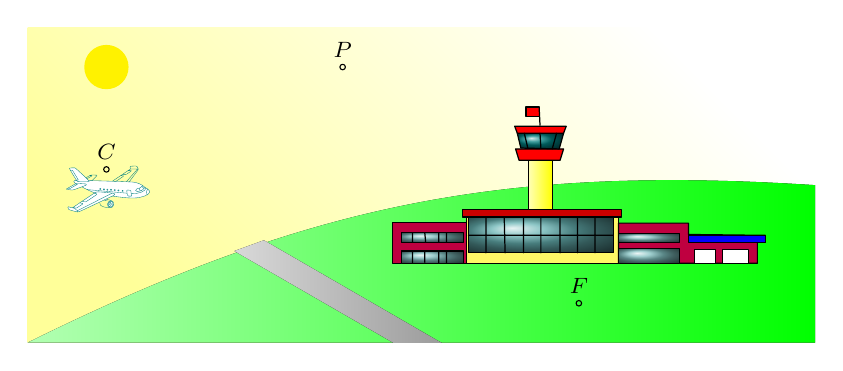
\begin{tikzpicture}[line cap=round,line join=round,>=stealth,font=\footnotesize]
				 \def\maybaymot{
				 \tikz{
				\draw[teal] (0.97,1.43).. controls+(0:0) and+(-162:0.06).. (1.17,1.5).. controls+(24:0.02)  and+(170:0.02).. (1.23,1.5).. controls+(-10:0.06) and+(169:0.06).. (1.43,1.46).. controls+(-10:0.02) and+(36:0.02).. (1.44,1.43).. controls+(-144:0.06) and+(0:0).. (1.19,1.26)
					 (1,1.38).. controls+(0:0) and+(-156:0.04).. (1.23,1.46).. controls+(18:0) and+(-18:0).. (1.22,1.47).. controls+(171:0.02) and+(0:0).. (1.14,1.49);
				\draw[teal] (2.03,1.09).. controls+(0:0) and+(-157:0.08).. (2.86,1.46).. controls+(18:0) and+(-90:0).. (2.87,1.47).. controls+(90:0) and+(-95:0.02).. (2.87,1.55)..  controls+(90:0.02) and+(173:0.02).. (2.9,1.58).. controls+(-4:0.06) and+(173:0.06).. (3.12,1.55).. controls+(-11:0.04) and+(105:0.02).. (3.17,1.51).. controls+(-75:0.04) and+(106:0.02).. (3.19,1.42).. controls+(-73:0.02) and+(39:0.02).. (3.18,1.37).. controls+(-136:0.12) and+(0:0).. (2.72,0.94)
					 (2.61,0.97)--(3.16,1.41)--(3.15,1.42)--(2.9,1.46)
					(2.77,1.41).. controls+(0:0) and+(174:0.04).. (2.89,1.4).. controls+(-7:0.02) and+(27:0.02)..  (2.89,1.38).. controls+(-156:0.04) and+(23:0.08).. (2.68,1.28).. controls+(-158:0.02) and+(-10:0.02).. (2.64,1.28).. controls+(170:0.04) and+(0:0).. (2.51,1.3)
					(2.41,1.26).. controls+(0:0) and+(170:0.02).. (2.53,1.24).. controls+(-11:0.02) and+(29:0.02).. (2.53,1.22).. controls+(-152:0.08) and+(0:0)..  (2.18,1.06);
				\def\than{(1.23,0.74).. controls+(158:0.14) and+(-41:0.2).. (0.47,1.3).. controls+(140:0.06) and+(-173:0.06).. (0.49,1.4).. controls+(0:0.02) and+(170:0.02).. (0.56,1.39).. controls+(-10:0.54) and+(168:0.64).. (2.84,0.92).. controls+(-12:0.2) and+(125:0.18).. (3.34,0.6)..  controls+(-32:0.08) and+(73:0.06).. (3.5,0.38).. controls+(-106:0.14) and+(-3:0.2).. (2.92,0.23).. controls+(177:0.38) and+(-22:0.44).. (1.23,0.74)--cycle
				} 
				\draw[teal,fill=white] \than; 
				\draw[teal,fill=white](0.61,1.33).. controls+(-17:0.02) and+(-97:0.04).. (1.08,1.26).. controls+(83:0.04) and+(-54:0.18)..  (0.62,1.89).. controls+(126:0.02) and+(-6:0.02).. (0.58,1.92).. controls+(168:0.04) and+(63:0.02).. (0.36,1.94).. controls+(-119:0.02) and+(111:0.2).. (0.57,1.37).. controls+(-67:0.02) and+(162:0.02).. (0.61,1.33)--cycle;
				\draw[teal] (0.38,1.84).. controls+(0:0)  and+(170:0.02).. (0.47,1.83).. controls+(0:0) and+(117:0).. (0.47,1.83).. controls+(-66:0.02) and+(111:0.04).. (0.64,1.4).. controls+(-63:0) and+(-27:0).. (0.63,1.39).. controls+(180:0) and+(-12:0.02).. (0.56,1.4);
				\draw[teal,fill=white](0.56,1.26).. controls+(-13:0.1) and+(165:0.1).. (0.9,1.18).. controls+(-14:0.04) and+(11:0.04).. (0.92,1.12).. controls+(-168:0.14) and+(10:0.12).. (0.43,1.03).. controls+(-168:0.02) and+(-12:0.02).. (0.32,1.02)..  controls+(164:0.06) and+(-17:0.06).. (0.09,1.09).. controls+(164:0.02) and+(-157:0.02).. (0.09,1.11).. controls+(20:0.1) and+(-160:0.12).. (0.51,1.26).. controls+(21:0.02) and+(166:0.02).. (0.56,1.26)--cycle;
				\draw[teal] (0.49,1.25).. controls+(0:0)  and+(165:0.02).. (0.56,1.23).. controls+(-11:0.02) and+(14:0).. (0.57,1.22).. controls+(-160:0.06) and+(20:0.06).. (0.26,1.11).. controls+(-160:0.02) and+(-16:0.02).. (0.22,1.1).. controls+(162:0.02) and+(0:0).. (0.14,1.12);
				\draw[teal] (1.78,0.01).. controls+(174:0.08)  and+(-32:0.08).. (1.45,0.12).. controls+(148:0.08) and+(-103:0.12).. (1.36,0.32);
				 \draw[teal] (1.84,0.31).. controls+(148:0.08) and+(-21:0.08).. (1.62,0.4);
				\draw[teal,fill=white](1.67,0.19).. controls+(83:0.06) and+(162:0.06).. (1.84,0.31).. controls+(-18:0.1) and+(75:0.06).. (1.92,0.12).. controls+(-105:0.06) and+(-18:0.06).. (1.77,0.01).. controls+(162:0.12)  and+(-96:0.08).. (1.67,0.19)--cycle;
				\draw[teal] (1.7,0.18).. controls+(79:0.06) and+(169:0.06).. (1.83,0.28).. controls+(-12:0.08) and+(74:0.08).. (1.89,0.12).. controls+(-105:0.04) and+(-4:0.06)..  (1.78,0.04).. controls+(177:0.06) and+(-100:0.08).. (1.7,0.18)--cycle;
				 \draw[teal,fill=white] (1.66,0.41).. controls+(0:0) and+(56:0.02).. (1.69,0.35).. controls+(-128:0.04) and+(0:0).. (1.55,0.38);
				\draw[teal] (1.74,0.25).. controls+(-24:0.04) and+(72:0.04)..  (1.79,0.17).. controls+(-108:0.04) and+(-13:0.06).. (1.7,0.13)
					(1.79,0.28)..  controls+(-31:0.04) and+(77:0.04).. (1.83,0.16).. controls+(-103:0.06) and+(-4:0.06).. (1.72,0.07);
				\draw[teal,fill=white](0.39,0.11)--(0.3,0.23)--(0.28,0.25).. controls+(0:0) and+(-25:0.06).. (0.03,0.36).. controls+(157:0.02) and+(97:0.02).. (0.01,0.34).. controls+(-79:0.04) and+(114:0.02).. (0.03,0.25).. controls+(-68:0.02) and+(150:0.02).. (0.07,0.22).. controls+(-27:0.06)  and+(161:0.1).. (0.37,0.08).. controls+(-16:0.02) and+(-163:0.02).. (0.45,0.08).. controls+(14:0.28) and+(-164:0.2).. (1.99,0.5).. controls+(15:0.08) and+(-19:0.08).. (1.99,0.59).. controls+(162:0.16) and+(-14:0.16).. (1.37,0.76).. controls+(166:0.04) and+(24:0.04).. (1.27,0.76).. controls+(-157:0.3) and+(0:0).. (0.2,0.29);
				\draw[teal]  (0.38,0.13)--(1.93,0.6)
					(0.22,0.3).. controls+(0:0) and+(156:0.02).. (0.33,0.25).. controls+(-18:0.02) and+(-162:0.02).. (0.37,0.25).. controls+(24:0.04) and+(-155:0.06).. (0.65,0.37).. controls+(23:0.02)  and+(-27:0.02).. (0.65,0.39).. controls+(161:0.04) and+(0:0).. (0.54,0.44)
					(0.65,0.48).. controls+(0:0) and+(162:0.04).. (0.76,0.44).. controls+(-18:0.02) and+(-157:0.02).. (0.8,0.44).. controls+(23:0.1) and+(-155:0.08).. (1.3,0.66)..  controls+(23:0.02) and+(-18:0.02).. (1.3,0.69).. controls+(163:0.04) and+(0:0).. (1.19,0.72)
					(0.94,0.93)--(2.75,0.44).. controls+(-11:0.32)  and+(-112:0.14).. (3.38,0.57);
				\draw[teal,fill=white](2.73,0.56).. controls+(-102:0.04) and+(100:0.04).. (2.73,0.37).. controls+(-82:0.02) and+(-4:0.02).. (2.71,0.34)--(2.6,0.36).. controls+(163:0.02) and+(-84:0.02).. (2.56,0.4).. controls+(99:0.06) and+(-111:0.06).. (2.57,0.61)..  controls+(68:0.02) and+(174:0.02).. (2.6,0.62)--(2.71,0.59).. controls+(-23:0.02) and+(78:0.02).. (2.73,0.56)--cycle;
				\draw[teal] (3.44,0.52).. controls+(-146:0.08)  and+(103:0.12).. (3.37,0.27)
					(3.34,0.6).. controls+(-125:0.14) and+(-2:0.1)..  (3,0.48).. controls+(178:0.1) and+(-174:0.08).. (2.99,0.6).. controls+(6:0.1) and+(-133:0.12).. (3.26,0.69)
					(3.09,0.61)--(3.12,0.49)--(3.13,0.49) 
					 (3.22,0.65)--(3.3,0.56);
				 \foreach \x/\y in {1.48/0.86,1.63/0.82,1.77/0.78,1.92/0.75,2.07/0.71,2.39/0.62,2.22/0.67}
				 \draw[teal] (\x,\y) ellipse (0.03 and 0.03);
				} 
				} 
				\def\sanbay{\tikz{ 
				\draw[fill=purple] (0.10,0.65) -- (0.10,0.18) --  (0.95,0.18) -- (0.95,0.65) -- cycle;
				\draw[fill=yellow!60] (0.95,0.18) -- (0.95,0.71) -- (2.69,0.71) -- (2.69,0.18) -- cycle; 
				\draw[fill=purple] (2.69,0.64) -- (3.49,0.64) -- (3.49,0.51) -- (4.37,0.50) --  (4.37,0.42) -- (4.28,0.42) -- (4.28,0.18) -- (2.69,0.18) -- cycle;
				\draw[ball color=teal!50] (0.20,0.53)  -- (0.91,0.53) -- (0.91,0.42) -- (0.20,0.42) -- cycle;
				\draw[ball color=teal!50] (0.91,0.32)  -- (0.91,0.18) -- (0.20,0.18) -- (0.20,0.32) -- cycle;
				\draw[fill=red!80!black] (0.90,0.71) -- (2.72,0.71)  -- (2.72,0.80) -- (0.90,0.80) -- cycle;
				\draw[ball  color=teal!50] (2.69,0.52) -- (3.39,0.52) -- (3.39,0.42) -- (2.69,0.42) -- cycle;
				\draw[ball color=teal!50] (2.69,0.35) -- (3.39,0.35) -- (3.39,0.18) -- (2.69,0.18) --  cycle;
				\draw[fill=white] (3.56,0.18) -- (3.56,0.34) -- (3.80,0.34) --  (3.80,0.18) -- cycle;
				\draw[fill=white] (3.88,0.18) -- (3.88,0.34) -- (4.18,0.34)  -- (4.18,0.18) -- cycle;
				 \draw[fill=blue] (3.49,0.5) -- (4.37,0.5) -- (4.37,0.42) -- (3.49,0.42) -- cycle;
				\draw[ball color=teal!60] (0.97,0.71) -- (0.97,0.30) -- (2.63,0.30) -- (2.63,0.71) -- cycle; 
				\draw[left color=yellow!30,right color=yellow] (1.66,0.80) -- (1.66,1.36)  -- (1.93,1.36) -- (1.93,0.80) -- cycle;
				\draw[fill=red]  (1.51,1.49) -- (1.55,1.36) -- (2.02,1.36) -- (2.06,1.49) -- cycle;
				\draw[ball color=teal]  (1.53,1.67) -- (1.57,1.50) -- (2.01,1.49) -- (2.06,1.67) -- cycle;
				\draw[fill=red]  (1.50,1.75) -- (1.53,1.67) -- (2.06,1.67) -- (2.09,1.75) -- cycle;
				\draw[fill=red] (1.78,1.97)  -- (1.63,1.97) -- (1.63,1.86) -- (1.78,1.86);
				\draw 
					(0.33,0.53)--(0.33,0.42) 
					(0.47,0.53)--(0.48,0.42) 
					(0.63,0.53)--(0.63,0.42) 
					(0.72,0.53)--(0.72,0.42) 
					 (0.72,0.32)--(0.72,0.18)
					(0.63,0.32)--(0.63,0.18) 
					(0.47,0.32)--(0.47,0.19) 
					(0.33,0.32)--(0.33,0.18) 
					(1.17,0.71)--(1.17,0.30) 
					(1.38,0.71)--(1.39,0.30) 
					 (1.60,0.71)--(1.60,0.30)
					(1.80,0.71)--(1.80,0.30) 
					 (2.02,0.71)--(2.02,0.30)
					 (2.22,0.71)--(2.22,0.30)
					 (2.42,0.71)--(2.42,0.30)
					 (0.97,0.50)--(2.63,0.50)
					(1.61,1.67)--(1.65,1.50) 
					 (1.79,1.67)--(1.80,1.50)
					 (1.98,1.67)--(1.93,1.49)
					 (1.79,1.76)--(1.78,1.97);
					 }}
				\clip (0,0) rectangle  (10,4);
				\shade[shading=axis,left  color=yellow!40,right color=white,shading angle=135] (0,0) rectangle (10,4);
				\fill[yellow] (1,3.5) circle (8pt); 
			\fill[left color=green!30,right color=green] (0,0) to[bend left= 15] (10,2)--(10,0)--cycle;
			\fill[left  color=gray!30,right color=gray] (3,1.3)--++(-30:4)--++(-160:0.4)--++(150:4)--cycle;
			 \path (1,2) node[rotate=10] (nB) {\resizebox{!}{0.6cm}{\maybaymot}};
			\path (7,2) node (sB) {\resizebox{!}{2cm}{\sanbay}}; 
			\path 
				(1,2.2) coordinate  (C)
				(7,0.5) coordinate (F) 
				(4,3.5)  coordinate (P);
			\foreach \x in{C,F,P}{\draw  (\x) circle (1pt) node[above] {$\x$};}
		\end{tikzpicture}
	\end{center}
	\shortans{0,95} 
	 \loigiai{
		Sau khi qua $C$, Beta bay theo hướng $\overrightarrow{w}=(-5;4;-1)$  có phương trình là $\heva{&x=10-5\lambda\\ &y=-10+4\lambda\\ &z=5-\lambda.}$\\
		 Ở cao $1\,000$\,m $=1$\,km ta có $5-\lambda=1\Rightarrow\lambda=4$.\\
		Điểm đổi hướng cuối là  $P(-10;6;1)$.\\
		Chặng cuối hướng về $F(-12;7;0)$ có vectơ chỉ phương  $\overrightarrow{PF}=\overrightarrow{u}=(-2;1;-1)$.\\
		Khi  đó $\cos\theta=\dfrac{\overrightarrow{w}\cdot\overrightarrow{u}}{\left|\overrightarrow{w}\right|\cdot\left|\overrightarrow{u}\right|}=\dfrac{10+4+1}{\sqrt{42}\cdot\sqrt{6}}=\dfrac{15}{\sqrt{252}}\approx0{,}95$.
	 }
\end{bt}

% nguồn: Phan2_Lop_12_Hinh_hoc_Chuong_5
\begin{bt}%[2H5V2-8]%[ma:5d4ee879]
	 Trong một trung tâm nghiên cứu robot bay, người ta bố trí một thiết bị định vị tại điểm cố định $A(1;0;2)$ trong không gian ba chiều với hệ tọa độ $Oxyz$ (các đơn vị tọa độ được tính bằng mét). Thiết bị này giao tiếp đồng thời với hai cảm biến: Cảm biến thứ nhất di chuyển dọc theo đường thẳng $\Delta\colon \dfrac{x-3}{1} = \dfrac{y+1}{2} = \dfrac{z-4}{-1}$, cảm biến thứ hai được gắn trên mặt phẳng $(\alpha)\colon 2x-y+z+1=0$. Giữa hai cảm biến được kết nối bằng một đường truyền $BC$, trong đó $B$ nằm trên đường thẳng $\Delta$, $C$ nằm trên mặt phẳng $(\alpha)$ và thiết bị định vị tại $A$ là trung điểm của đoạn $BC$. Biết rằng đường thẳng $BC$ có một véc-tơ chỉ phương $\overrightarrow{u}=(-2;a;b)$, hãy tính giá trị $a+2b$.
	 \shortans{-1,5}
	 \loigiai{
		 Vì $B \in \Delta$ nên $B(3+t; -1+2t; 4-t)$.\\
		Gọi  $C\left(x_C; y_C; z_C \right)$.\\
		Vì $A(1;0;2)$ là trung điểm  của $BC$ nên
		\[\heva{&1=\dfrac{3+t+x_C}{2}\\&0=\dfrac{-1+2t+y_C}{2}\\&2=\dfrac{4-t+z_C}{2}} 
		 \Leftrightarrow
		\heva{&x_C=-1-t\\&y_C=1-2t\\&z_C=t}\Leftrightarrow  C(-1-t;1-2t;t). \]
		Ta  có $C(-1-t;1-2t;t)\in (\alpha)$ nên $2(-1-t)-(1-2t)+t+1=0 \Leftrightarrow t=2$.\\
		Khi  đó $B(5;3;2)$ và $C(-3;-3;2)$.\\
		Suy ra $\overrightarrow{BC} = (-8;-6;0)$, chọn $\overrightarrow{u} =  (-2; -1{,}5; 0)$.\\
		Khi đó $a=-1{,}5$ và $b=0$,  suy ra $a+2b=-1{,}5$.
	 }
\end{bt}

% nguồn: Phan2_Lop_12_Hinh_hoc_Chuong_5
\begin{bt}%[2H5V2-8]%[ma:6db5d965]
	Tháp gồm một khối lập phương, trên đó gắn thêm một khung hộp chữ nhật, và phía trên là  một khối chóp tứ giác đều. Tại độ cao bằng chiều cao khối lập phương, có gắn một mặt phẳng trượt hình chữ nhật (xem hình, các kích thước tính bằng mét).\\
	\begin{center}
		\begin{tikzpicture}[line join = round,line cap=round,>=stealth,font=\footnotesize,scale=1]
				 \path
					(0,0) coordinate  (A)
					(1,1)  coordinate (D)
					 (3,1) coordinate (C)
					(2,0) coordinate (B) 
					($(A)+(0,2)$) coordinate  (E)
					($(B)+(0,2)$) coordinate  (F)
					($(C)+(0,2)$)  coordinate (G)
					 ($(D)+(0,2)$) coordinate (H)
					 ($(E)+(0,1.1)$) coordinate (E1)
					($(F)+(0,1.1)$) coordinate  (F1)
					 ($(G)+(0,1.1)$) coordinate (G1)
					($(H)+(0,1.1)$) coordinate (H1) 
					($(H1)!1/2!(F1)$) coordinate  (S1)
					 ($(S1)+(0,1)$) coordinate (S)
					 (8,1) coordinate (P1)
					($(P1)+(-0.5,-0.5)$) coordinate (P); 
				\foreach  \p/\r in {A/-90,B/-90,C/-30,D/-180,E/-180,H/-45,G/-90,F/-135,S/90,P/-90}
				\fill  (\p) circle (1.2pt) node[shift={(\r:3mm)}]{$\p$};
				\draw[fill=yellow,opacity=0.3] (E)--(F)--(G)--(H)--cycle--(A)--(B) node[midway,below]{$2$}--(C) node[midway,right]{$2$}--(G) 
					(E)--(A)  node[midway,left]{$2$}
					(F)--(B) 
					(G)--(C); 
				\draw[dashed]  (A)--(D)--(C)
					(D)--(H) 
					(P)--(P1) node[above]{$7$}; 
				\draw[line width=1.25pt,red] (E)--(E1)  node[midway,left]{$1$}
					(F)--(F1) 
					 (G)--(G1);
				 \draw[fill=green,opacity=0.2] (S)--(E1)--(F1)--(G1)--(S)--(F1);
				\draw[fill=cyan,opacity=0.5] (G)--++(3,-2)  node[above]{$5$}--++(-1,-1)--(F)--cycle;
				\draw[cyan,line  width=1pt] (S)--(P);
				\draw[->]  (A)--++(-0.5,-0.5) node[left]{$x$};
				\draw[->] (C)--++(6,0)  node[below]{$y$};
				 \draw[->] (H)--++(0,2) node[left]{$z$};
			\end{tikzpicture}
	\end{center}
	Từ đỉnh $S$ có buộc một sợi dây xuống điểm $P(1;7;0)$ làm dây leo.\\ 
	Trên mặt phẳng trượt,  có một đứa trẻ đứng thẳng tại vị trí chính giữa tấm trượt và với thẳng tay (vuông góc với mặt đất) nắm được dây leo. Tính chiều cao tay vịn của đứa trẻ tính từ mặt đất.
	 \shortans{1,6}
	\loigiai{ 
		Ta xác định được tọa  độ các điểm như sau $D(0;0;0)$, $A(2;0;0)$, $B(2;2;0)$, $C(0;2;0)$, $H(0;0;2)$, $E(2;0;2)$, $F(2;2;2)$, $G(0;2;2)$, $S(1;1;4)$.\\
		Phương trình đường thẳng $SP\colon  \heva{& x = 1 \\&y = 1+6t \\&z = 4-4t}$ ($t \in \mathbb{R}$).\\
		Ta thấy mặt phẳng trượt đi qua $F$, $G$, $K(0;5;0)$ nên phương trình  mặt phẳng trượt là $2y+3z-10=0$.\\
		Điểm chính giữa tấm trượt có tọa độ  $I(1;3{,}5;1)$.\\
		Đứa trẻ đứng thẳng tại vị trí chính giữa tấm trượt và với thẳng tay (vuông góc với mặt  đất) thuộc đường thẳng có vectơ chỉ phương $(0;0;1)$ và đi qua $I(1;3{,}5;1)$.\\
		Phương trình  $\Delta\colon \heva{&x = 1 \\&y = 3{,}5 \\&z = 1+k}$ ($k \in \mathbb{R}$).\\
		Tìm giao điểm $\Delta$ với $SP\colon \heva{&1 = 1 \\&3{,}5 = 1+6t \\&1+k =  4-4t}$ $\Leftrightarrow \heva{&t = 0{,}4 \\&k = 0{,}6.}$\\
		 Suy ra chiều cao tay vịn của đứa trẻ tính từ mặt đất là $1{,}6$ m.
	 }
\end{bt}

% nguồn: Phan2_Lop_12_Hinh_hoc_Chuong_5
\begin{bt}%[2H5V2-8]%[ma:b5f29f8c]
	Trực thăng cứu hộ Alpha cất cánh lúc $10$ giờ $00$ từ điểm xuất phát Adlerhorst $A(10;6;0)$. Nó bay thẳng với vận  tốc $300$\,km/h tới đỉnh núi Mount Devil $D(4;-3;3)$, nơi xảy ra tai nạn. (Tọa độ tính bằng km). Cùng lúc đó, trực thăng Beta cất cánh từ đỉnh núi Tempelberg $T(7;-8;3)$ để đưa du khách về điểm $B(4;16;0)$, vận tốc của nó là $350$\,km/h. Người ta chứng minh được rằng hai trực thăng có đường bay giao nhau tại $S$. Khi Alpha tới $S$ thì Beta đã đi qua trước đó một khoảng thời gian (tính bằng giây), hãy tìm khoảng thời gian đó? (làm tròn kết quả đến hàng phần mười).
	\begin{center}
		\begin{tikzpicture}[line cap=round,line join=round,>=stealth,font=\footnotesize]
				 \def\tt#1{
				 \tikz{
				\draw[fill=#1!80] (1.67,2.47) -- (1.73,2.37) -- (1.85,2.27) -- (1.97,2.17) -- (2.13,2.08) -- (2.33,2.00) -- (2.58,1.96) -- (3.04,1.90) -- (4.92,1.89) -- (5.59,1.98) -- (5.80,2.08) -- (6.08,2.24) -- (6.24,2.47) -- (6.38,2.83) -- (6.43,2.83) -- (6.43,3.30) -- (6.34,3.41) -- (6.20,3.53) -- (6.00,3.64) -- (5.78,3.74) -- (5.50,3.84) -- (5.21,3.92) --  (4.91,3.96) -- (4.62,4.00) -- (4.26,4.00) -- (3.79,4.04) -- (3.12,4.00) -- (2.97,3.95) -- (2.71,3.79) -- (2.87,3.87) -- (3.18,3.87) -- (3.41,3.86) -- (3.59,3.86) -- (3.84,3.85) -- (3.87,3.72) -- (3.42,2.33) -- (3.36,2.19) -- (3.24,2.11) -- (2.58,2.16) -- (2.45,2.20) -- (2.17,2.42) -- (2.04,2.48) -- cycle;
				\draw[ball color=teal] (1.67,2.47) -- (2.04,2.48) -- (2.17,2.42) -- (2.45,2.20) -- (2.58,2.16) -- (3.24,2.11) --  (3.36,2.19) -- (3.42,2.33) -- (3.87,3.72) -- (3.84,3.85) -- (3.59,3.86) -- (3.41,3.86) -- (3.18,3.87) -- (2.87,3.87) -- (2.71,3.79) -- (2.59,3.65) -- (2.47,3.52) -- (2.32,3.33) -- (2.15,3.10) -- (2.06,2.93) -- (1.93,2.88) -- (1.83,2.78) -- (1.73,2.67) -- (1.68,2.56) -- cycle;
				\draw (4.00,3.80) -- (3.88,3.51) -- (3.77,3.20) -- (3.67,2.86) -- (3.56,2.46) -- (3.51,2.30) -- (3.51,2.17) -- (3.56,2.10) -- (5.21,2.12) -- (5.29,2.28) -- (5.34,2.46) -- (5.39,2.70) -- (5.43,3.03) -- (5.45,3.45) -- (5.42,3.71) -- (5.35,3.75)  -- (5.13,3.82) -- (4.88,3.85) -- (4.60,3.88) -- (4.34,3.88) -- (4.10,3.89) -- cycle;
				 \draw[fill=#1] (1.67,2.47)--(1.68,2.56)--(1.73,2.67)--(1.83,2.78)--(1.93,2.88)--(2.06,2.93)--(2.21,2.94)--(2.34,2.94)--(2.42,2.93)--(2.47,2.93)--(2.58,2.89)--(2.69,2.83)--(2.77,2.75)--(2.84,2.67)--(2.88,2.56)--(2.90,2.45)--(2.88,2.38)--(2.82,2.29)--(2.76,2.24)--(2.68,2.19)--(2.58,2.16)--(2.45,2.20)--(2.17,2.42)--(2.04,2.48);
				\draw[fill=#1] (3.27,3.87) -- (3.09,3.73) -- (2.94,3.60) -- (2.79,3.44) -- (2.67,3.29) -- (2.58,3.17) -- (2.51,3.06) -- (2.42,2.93) -- (2.34,2.94) -- (2.26,2.94) -- (2.34,3.02) -- (2.38,3.09) -- (2.45,3.19) -- (2.53,3.28) -- (2.60,3.37)  -- (2.74,3.54) -- (2.87,3.67) -- (3.00,3.80) -- (3.09,3.87) -- cycle;
				\draw[ball color=teal] (4.11,3.77) -- (4.20,3.80) -- (4.75,3.77) -- (4.82,3.71) -- (4.81,3.17) -- (4.79,3.04) -- (4.76,2.89) -- (4.70,2.83) -- (3.86,2.59) -- (3.80,2.60) -- (3.74,2.65) -- (3.76,2.78) -- (3.86,3.15) -- (3.96,3.46) -- (4.05,3.68)  -- cycle;
				\draw[ball color=teal] (5.18,3.66) -- (5.28,3.65) -- (5.31,3.60) -- (5.35,3.48) -- (5.36,3.33)  -- (5.34,3.22) -- (5.29,3.19) -- (5.17,3.19) -- (5.15,3.26) -- (5.14,3.54) -- cycle;
				\draw[fill=#1!70] (5.86,3.70) -- (6.31,3.69) -- (6.37,3.78) -- (8.42,3.70) -- (8.83,4.78) -- (8.89,4.89) -- (8.96,4.92) -- (9.26,4.92) -- (9.29,4.88) -- (9.28,4.82) -- (9.07,3.85) -- (9.15,3.79) -- (9.21,3.74) -- (9.22,3.68) -- (9.23,3.61) -- (9.27,3.55) -- (9.59,3.55) -- (9.67,3.51) -- (9.67,3.38) -- (9.62,3.32) -- (9.29,3.32) -- (9.24,3.25) -- (9.24,3.18) -- (9.22,3.08) --  (9.13,2.98) -- (9.03,2.94) -- (8.92,2.93) -- (9.01,2.73) -- (9.27,2.71) -- (9.31,2.63) -- (9.00,2.50) -- (8.87,2.54) -- (8.60,2.83) -- (8.43,2.92) -- (8.12,3.17) -- (6.43,2.83) -- (6.43,3.30) -- (6.34,3.41) -- (6.20,3.53) -- (6.00,3.64) -- cycle;
				\fill[yellow!80!black] (8.42,3.70) -- (8.58,3.81) -- (8.71,3.87) -- (9.03,4.66) -- (9.26,4.72) -- (9.28,4.82) -- (9.29,4.88)  -- (9.26,4.92) -- (8.96,4.92) -- (8.89,4.89) -- (8.83,4.78) -- cycle;
				\draw[fill=orange!40!#1] (8.12,3.17) -- (8.61,3.28) -- (8.64,3.17)  -- (8.70,3.08) -- (8.80,3.00) -- (8.92,2.93) -- (9.01,2.73) -- (9.27,2.71) -- (9.31,2.63) -- (9.00,2.50) -- (8.87,2.54) -- (8.60,2.83) -- (8.43,2.92) -- cycle;
				\draw[fill=#1!70!black] (8.61,3.28) -- (8.61,3.45) -- (8.63,3.62) -- (8.74,3.75) -- (8.86,3.85) -- (8.99,3.85) -- (9.07,3.85) -- (9.15,3.79) -- (9.22,3.68) -- (9.23,3.61) -- (9.27,3.55) -- (9.59,3.55) -- (9.67,3.51) -- (9.67,3.38) -- (9.62,3.32) -- (9.29,3.32) -- (9.24,3.25) -- (9.24,3.18) -- (9.22,3.08) -- (9.13,2.98) -- (9.03,2.94) --  (8.92,2.93) -- (8.80,3.00) -- (8.70,3.08) -- (8.64,3.17) -- cycle;
				\draw[fill=#1!70]  (3.79,4.04) -- (3.96,4.23) -- (4.13,4.34) -- (4.33,4.39) -- (4.67,4.42) -- (5.37,4.41) -- (5.50,4.35) -- (6.09,4.35) -- (6.21,4.30) -- (6.33,4.24) -- (6.39,4.09) -- (6.37,3.78) -- (6.31,3.69) -- (5.86,3.70) -- (5.78,3.74) -- (5.50,3.84) -- (5.21,3.92) -- (4.91,3.96) -- (4.62,4.00) -- (4.26,4.00) -- cycle;
				\fill[#1!90!red] (4.26,4.00) -- (4.25,4.09) -- (4.36,4.20) -- (4.47,4.25) -- (4.61,4.29) --  (5.17,4.29) -- (5.34,4.29) -- (5.48,4.30) -- (5.58,4.27) -- (5.65,4.18) -- (5.63,4.26) -- (5.61,4.31) -- (5.56,4.33) -- (5.50,4.35) -- (5.37,4.41) -- (4.67,4.42) -- (4.33,4.39) -- (4.13,4.34) -- (3.96,4.23) -- (3.79,4.04) -- cycle;
				\draw[ball color=orange] (5.65,4.18) -- (5.69,4.14) -- (5.70,4.04) -- (5.71,3.84) --  (5.71,3.76) -- (5.78,3.74) -- (5.86,3.70) -- (5.95,3.74) -- (6.03,3.80) -- (6.07,3.89) -- (6.09,4.00) -- (6.07,4.09) -- (6.00,4.20) -- (5.99,4.28) -- (5.97,4.35) -- (5.50,4.35) -- (5.56,4.33) -- (5.61,4.31) -- (5.63,4.26) -- cycle;
				\draw[ball color=blue]  (9,3.39) ellipse ({0.15} and {0.3});
				\draw[ball color=#1] (6.55,2.86) -- (6.57,2.98) -- (6.57,3.11) -- (6.57,3.24) --  (6.54,3.36) -- (6.41,3.53) -- (8.19,3.53) -- (8.22,3.47) -- (8.23,3.42) -- (8.23,3.35) -- (8.21,3.29) -- (8.20,3.23) -- (8.12,3.17) -- cycle;
				\draw[fill=red] (7.04,3.35)  -- (7.27,3.36) -- (7.28,3.33) -- (7.29,3.30) -- (7.28,3.28) -- (7.27,3.25) -- (7.24,3.24) -- (7.06,3.24) -- (7.04,3.25) -- (7.02,3.27) -- (7.01,3.30) -- (7.02,3.34) -- cycle;
				\draw[fill=#1] (4.20,3.80) -- (4.21,3.74) -- (4.21,3.63) -- (4.21,3.52) -- (4.20,3.40) -- (4.19,3.27) -- (4.17,3.13) -- (4.14,2.99) -- (4.10,2.85)  -- (4.04,2.64) -- (4.11,2.66) -- (4.17,2.84) -- (4.20,2.96) -- (4.23,3.08) -- (4.24,3.17) -- (4.26,3.28) -- (4.27,3.38) -- (4.28,3.48) -- (4.28,3.58) -- (4.27,3.66) -- (4.28,3.75) -- (4.26,3.80) -- cycle;
				\draw[fill=cyan] (4.64,4.41) -- (4.64,4.47) -- (4.60,4.50) -- (4.60,4.60)  -- (4.90,4.60) -- (4.90,4.50) -- (4.87,4.48) -- (4.87,4.41) -- cycle;
				\draw[fill=gray] (4.65,4.60) -- (4.85,4.60) -- (4.84,5.03)  -- (5.01,5.04) -- (5.05,5.13) -- (5.29,5.13) -- (5.29,5.21) -- (5.12,5.31) -- (4.90,5.36) -- (4.60,5.37) -- (4.41,5.31) -- (4.23,5.22) -- (4.23,5.13) -- (4.49,5.13) -- (4.52,5.04) -- (4.65,5.04) -- cycle;
				\draw[fill=teal] (4.84,4.79) -- (5.11,4.79) -- (5.16,4.72) -- (5.22,4.72) --  (5.25,4.79) -- (5.52,4.79) -- (5.52,4.99) -- (4.84,4.99) -- cycle;
				\draw[fill=teal] (4.63,4.99) --  (4.00,5.00) -- (4.00,4.80) -- (4.26,4.80) -- (4.29,4.73) -- (4.33,4.73) -- (4.36,4.80) -- (4.64,4.80) -- cycle;
				\draw (5.52,4.99) -- (5.84,5.00) -- (6.11,5.10) -- (6.48,5.17) -- (7.27,5.24) -- (7.81,5.26) -- (8.57,5.27) -- (9.28,5.27) -- (9.64,5.25) -- (9.79,5.21) -- (9.79,5.13) -- (9.70,5.11) -- (9.53,5.08) -- (9.14,5.07) -- (8.58,5.06) -- (8.16,5.04) -- (7.63,5.01) -- (7.20,5.00) -- (6.78,4.97) -- (6.29,4.91)  -- (6.76,4.84) -- (7.37,4.75) -- (7.88,4.69) -- (8.38,4.62) -- (8.75,4.56) -- (8.71,4.45) -- (8.38,4.47) -- (7.88,4.53) -- (7.42,4.58) -- (6.98,4.63) -- (6.59,4.69) -- (6.16,4.75) -- (5.82,4.78) -- (5.71,4.82) -- (5.52,4.83) -- cycle;
				\draw (4.00,5.00) -- (3.80,5.00) -- (3.48,5.04) -- (3.15,5.11) -- (2.65,5.17) -- (2.05,5.19) -- (1.33,5.23) -- (0.69,5.23) -- (0.47,5.20) -- (0.43,5.13) -- (0.50,5.07) -- (1.11,5.04) -- (1.73,5.02) -- (2.48,4.99) -- (3.12,4.95) -- (3.80,4.91) -- (3.20,4.88) -- (2.62,4.85) -- (2.00,4.80) -- (1.32,4.72) -- (0.78,4.64) -- (0.63,4.61) -- (0.58,4.56) -- (0.71,4.53) -- (1.40,4.60) -- (2.20,4.67) -- (3.02,4.74) -- (3.90,4.83)  -- (4.00,4.84) -- cycle;
				\draw[fill=#1]  (4.49,5.13) -- (5.05,5.13) -- (5.29,5.13) -- (5.29,5.21) -- (5.12,5.31) -- (4.90,5.36) -- (4.60,5.37) -- (4.41,5.31) -- (4.23,5.22) -- (4.23,5.13) -- cycle;
				\draw[fill=black!60] (2.58,1.96)--(2.45,1.80)--(2.39,1.70)--(2.39,1.55)--(2.35,1.54)--(2.25,1.60)--(2.10,1.75)--(2.03,1.78)--(1.97,1.74)--(1.97,1.67)--(2.03,1.59)--(2.31,1.38)--(2.39,1.35)--(4.47,1.42)--(4.40,1.52)--(4.40,1.60)--(4.44,1.64)--(4.52,1.62)--(4.57,1.57)--(4.80,1.89)--(4.62,1.89)--(4.36,1.58)--(4.25,1.58)--(4.10,1.90)--(3.95,1.90)--(4.09,1.59)--(2.53,1.52)--(2.50,1.56)--(2.50,1.69)--(2.72,1.94); 
				\draw[fill=black!80]  (4.80,1.20)--(4.72,1.23)--(4.47,1.42)--(4.40,1.52)--(4.40,1.60)--(4.44,1.64)--(4.52,1.62)--(4.57,1.57)--(4.80,1.40)--(4.87,1.48)--(4.90,1.57)--(4.93,1.68)--(4.92,1.74)--(4.91,1.80)--(4.86,1.89)--(4.99,1.91)--(5.03,1.84)--(5.05,1.78)--(5.05,1.69)--(5.04,1.61)--(5.02,1.53)--(4.99,1.46)--(4.96,1.41)--(6.30,1.46)--(6.26,1.62)--(6.18,1.74)--(6.08,1.86)--(5.97,1.98)--(5.80,2.08)--(5.97,2.18)--(6.11,2.08)--(6.19,1.99)--(6.27,1.90)--(6.34,1.80)--(6.41,1.66)--(6.44,1.55)--(6.45,1.47)--(6.74,1.48)--(6.99,1.66)--(7.16,1.83)--(7.23,1.84)--(7.26,1.83)--(7.28,1.80)--(7.28,1.76)--(7.28,1.71)--(7.25,1.65)--(7.05,1.45)--(6.90,1.32)--(6.72,1.26)--cycle;
				\draw[ball  color=red] (4.88,2.77)--(4.69,2.76)--(4.65,2.69)--(4.72,2.63)--(4.85,2.61);
				 \draw (4.88,3.85)--(4.90,3.73)--(4.90,3.17)--(4.90,3.01)--(4.88,2.77)--(4.84,2.54)--(4.80,2.36)--(4.71,2.12);
				\draw  (5.21,3.92)--(5.21,4.23)--(5.24,4.26)--(5.31,4.26)--(5.33,4.24)--(5.34,3.88)--cycle;
					 }}
				\def\nui{ 
				 \tikz{
				\path[fill=gray!45!black] (0.22,0).. controls (-0.77,0.08) and (-1.66,0.63).. 
					(-2.37,1.29).. controls  (-2.52,1.42) and (-2.66,1.72)..
					(-2.61,1.38).. controls (-2.62,1.3) and (-2.63,1.22).. 
					(-2.59,1.16).. controls (-2.48,1.05)  and (-2.42,0.9)..
					 (-2.41,0.87).. controls (-2.41,0.8) and (-1.9,0.31)..
					(-1.88,0.33).. controls  (-1.99,0.29) and (-2.37,0.55)..
					(-2.48,0.7)..  controls (-2.59,0.49) and (-2.84,0.54)..
					 (-2.96,0.42).. controls (-3.07,0.31) and (-3.42,0.16)..
					(-3.44,0.19)..  controls (-3.46,0.21) and (-3.1,0.43)..
					(-3,0.57).. controls (-2.9,0.71) and  (-2.69,0.74)..
					(-2.66,0.78).. controls (-2.58,0.86) and  (-2.69,0.96)..
					 (-2.77,1.09).. controls (-2.83,1.2) and (-2.69,1.52)..
					 (-2.78,1.59).. controls (-2.85,1.49) and (-3.06,1.39)..
					(-3.25,1.2).. controls (-3.42,1.04) and (-3.48,1.26).. 
					(-3.9,0.86).. controls (-4.18,0.58) and  (-4.93,0.2)..
					 (-5,0.27).. controls (-4.98,0.31) and (-4.53,0.55)..
					(-4.34,0.73).. controls (-3.95,1.08) and (-3.81,1.24).. 
					(-3.65,1.29).. controls  (-3.37,1.36) and (-3.2,1.42)..
					(-2.91,1.79).. controls (-2.71,1.98) and (-2.45,1.7).. 
					(-2.23,1.45).. controls (-2.09,1.57)  and (-1.92,1.74)..
					(-1.82,1.83).. controls (-1.66,1.97) and (-1.61,2.12).. 
					(-1.48,2.25).. controls (-1.39,2.33)  and (-1.17,2.24)..
					(-1.08,2.31).. controls (-0.85,2.52)  and (-0.95,2.63)..
					 (-0.54,2.99).. controls (-0.19,3.3) and (-0.1,3.79)..
					(0.3,3.44).. controls (0.58,3.15) and  (0.73,2.69)..
					(1.15,2.54).. controls (1.56,2.36)  and (1.82,1.96)..
					(2.17,1.7)..  controls (2.34,1.91) and (2.65,2.1)..
					(2.89,1.86)..  controls (3.14,1.58) and (3.46,1.4)..
					(3.81,1.26).. controls (4.13,0.97)  and (4.43,0.65)..
					 (4.82,0.44).. controls (5.09,0.31) and (5.04,0.23)..
					(4.79,0.35).. controls  (4.37,0.5) and (4.04,0.8)..
					 (3.71,1.09).. controls (3.56,1.17) and (3.32,1.28)..
					(3.5,1.03).. controls (3.64,0.75) and  (3.13,1.39)..
					(3.2,1.32).. controls (3,1.38) and  (2.76,1.85)..
					 (2.61,1.69).. controls (2.87,1.42) and (2.33,1.01)..
					 (2.79,0.93).. controls (2.97,0.67) and (3.51,0.47)..
					 (3.6,0.33).. controls (3.18,0.4) and (2.87,0.7)..
					(2.5,0.87).. controls (2.18,1.03)  and (2.7,1.55)..
					(2.44,1.65).. controls (2.17,1.43)  and (1.96,1.14)..
					(1.68,0.93).. controls  (1.36,0.77) and (1.01,0.69)..
					(0.73,0.46).. controls (0.57,0.37) and (0.18,0.28).. 
					(0.11,0.36).. controls (0.5,0.45)  and (0.79,0.74)..
					(1.14,0.92).. controls (1.52,1.01) and  (1.78,1.29)..
					(2.03,1.57).. controls  (1.86,1.78) and (1.13,2.31)..
					(1.13,2.31).. controls (1.13,2.31) and (1.33,1.92).. 
					 (1.42,1.82).. controls (1.57,1.63) and (1.75,1.4)..
					(1.42,1.68).. controls  (1.09,1.93) and (0.95,2.35)..
					(0.64,2.63)..  controls (0.43,2.79) and (0.26,3.23)..
					(0.09,3.32).. controls (0.03,3.09) and (0.11,2.98).. 
					(0.08,2.83)..  controls (0.04,2.67) and (-0.08,2.6)..
					(-0.04,2.41).. controls (0.25,2.24) and (0.59,2.11).. 
					 (0.66,1.7).. controls (0.74,1.53) and (1.11,1.37)..
					(1.13,1.2)..  controls (0.95,1.36) and (0.62,1.47)..
					(0.55,1.62).. controls  (0.35,2.01) and (0.15,2.13)..
					 (0.02,2.16).. controls (0.26,1.65) and (-0.1,1.69)..
					 (-0.15,1.46).. controls (-0.16,1.18) and (0.45,1.09)..
					(0.42,0.73)..  controls (0.19,1.13) and (-0.3,1.01)..
					(-0.32,1.42).. controls (-0.33,1.77) and  (-0.11,1.68)..
					(-0.11,1.91).. controls (-0.11,2.08) and  (-0.31,2.22)..
					(-0.25,2.52).. controls (-0.21,2.77) and (-0.04,2.83).. 
					(-0.11,3.18).. controls (-0.38,2.83)  and (-0.79,2.52)..
					(-0.88,2.06).. controls (-0.94,1.71) and (-1.39,1.43).. 
					 (-1.42,1.19).. controls (-1.61,1.54) and (-0.97,1.84)..
					(-1.11,2.08).. controls (-1.36,2.15) and  (-1.32,1.94)..
					(-1.4,1.79).. controls (-1.39,1.88)  and (-1.41,1.94)..
					(-1.41,1.99).. controls (-1.46,1.91) and  (-1.73,1.5)..
					(-1.88,1.48).. controls (-2,1.42) and  (-1.96,1.38)..
					(-2.11,1.32)..  controls (-1.88,1.11) and (-1.62,0.99)..
					(-1.48,0.84).. controls (-0.82,0.36) and (-0.02,0.09).. 
					(0.79,0.04)..  controls (0.61,-0.01) and (0.4,0)..
					(0.22,0) -- cycle; 
				 }
				} 
				\tikzset{rada/.pic={ 
				\begin{scope}[rotate=40]
					 \fill (0,0) ellipse (1 and 1.2);
					\fill[white]  (0.5,0) ellipse (0.9 and 1.2);
					\fill (0.3,0)  ellipse (0.5 and 1.1);
					\draw[white,line width=0.2cm] ($(0.3,0)+(165:0.5 and  1.1)$)--++(-10:1.4);
					\draw[white,line width=0.2cm] ($(0.3,0)+(-165:0.5 and  1.1)$)--++(10:1.4);
					\filldraw[] ($(0.3,0)+(169:0.5 and 1.1)$)--(2,0)--($(0.3,0)+(-169:0.5 and  1.1)$);
					\fill (2,0) circle (0.2); 
					 \draw[line width=0.05cm] ($(0,0)+(30:3)$) arc (30:-30:3);
					\draw[line  width=0.05cm,shift={(0.5,0)}] ($(0,0)+(40:3.4)$) arc (40:-40:3.4);
					\draw[line width=0.05cm,shift={(0.5,0)}] ($(0,0)+(40:4)$)  arc (40:-40:4);
				\end{scope}
				\filldraw  ($(0,0)+(180:1 and 1.2)$)--++(-90:1.6)--++(-150:0.5)--++(-90:0.2)--++(-20:1)--++(30:1)--++(90:0.2)--++(160:0.5);
					}} 
				\pic[scale=0.3,xscale=-1] at (12,5)  {rada};
				 \path (5,5) node[anchor=south] (NUI) {\nui};
				\path (2.2,7) node[anchor=south,inner  sep=0pt,scale=.2,xscale=-1] (tt1) {\resizebox{!}{3cm}{\tt{orange}}};
				\path (7,3.5) node[anchor=south,inner sep=0pt,scale=.2]  (tt2) {\resizebox{!}{3cm}{\tt{yellow}}};
				\path 
					 (5,8.6) coordinate (D)
					(2.2,7) coordinate  (T)
					 (7,4) coordinate (A)
					(12,4.3)  coordinate (B);
				\draw[name path=fx,line  width=1pt,blue,dashed] (D)--(A);
				 \draw[name path=gx,line width=1pt,blue,dashed] (T)--(B);
				\draw[->,red] (4,5)--++(0:6) node[below] {$y$}; 
				 \draw[->,red] (4,5)--++(-135:3) node[below] {$x$};
				\draw[->,red] (4,5)--++(90:4) node[left] {$z$}; 
				\path[name intersections={of=fx and gx}] (intersection-1) coordinate (S)  node[below] {$S$};
				\foreach \x/\y in {A/above,B/below,D/above,T/left}{\draw[fill=red] (\x) circle (1pt) node[\y]  {$\x$};}
			\end{tikzpicture}
	\end{center}
	 \shortans{6,4}
	\loigiai{ 
		Đường bay của Alpha đi qua điểm $A(10;6;0)$, hướng $\overrightarrow{AD}=(-6;-9;3)$ nên có phương trình  \[d_{\alpha}\colon\heva{&x=10-6t\\&y=6-9t\\&z=0+3t.}\]
		 Đường bay của Beta đi qua điểm
		$T(7;-8;3)$,  hướng $TB=(-3; 24;-3)$ nên có phương trình \[d_{\beta}\colon\heva{&x=7-3s\\&y=-8+24s\\ &z=3-3s.}\]
		Giao  điểm đường bay $d_{\alpha}$ và $d_{\beta}$ là nghiệm của hệ phương trình \[\heva{&10-6t=7-3s\\&6-9t=-8+24s\\&0+3t=3-3s}\Leftrightarrow \heva{&r=\dfrac{2}{3}\\&s=\dfrac{1}{3}.}\]
		Suy ra $d_{\alpha}$ và  $d_{\beta}$ giao nhau tại điểm $S(6;0;2)$.\\
		\begin{itemize}
			\item  Quãng đường từ Adlerhorst tới điểm $S$ là \[\left|AS\right|=\sqrt{(-4)^2+(-6)^2+2^2}=\sqrt{56}\approx7{,}48\,\mathrm{km}.\]
			\item Quãng đường từ  đỉnh núi Tempelberg tới điểm $S$ là \[\left|TS\right|=\sqrt{(-1)^2+8^2+(-1)^2}=\sqrt{66}\approx8{,}12\,\mathrm{km}.\]
			\item Thời gian bay từ Adlerhorst tới điểm $S$ là $t_{\alpha}=\dfrac{7{,}48}{300}\approx 0{,}025$\,h $\approx 1{,}50$  phút.
			 \item Thời gian bay từ đỉnh núi Tempelberg tới điểm $S$ là $ t_{\beta}=\dfrac{8{,}12}{350}$\,h $\approx0{,}023$\,h $\approx1{,}39$ phút.
		\end{itemize}
		Vậy Alpha tới  $S$ muộn hơn Beta một khoảng $0{,}11$ phút $\approx 6{,}45$\,s.
	 }
\end{bt}

% nguồn: Phan2_Lop_12_Hinh_hoc_Chuong_5
\begin{bt}%[2H5V2-8]%[ma:45e472a3]
	\immini{Trong không gian với hệ trục tọa độ $Oxyz$, mỗi đơn vị trên hệ trục ứng với $10$\,km, trạm kiểm soát không lưu đang theo dõi hai máy bay. Máy bay thứ nhất ban đầu ở tọa độ $A(25;-10;1)$ và bay theo hướng vectơ $\overrightarrow{v}_1=(-3;-4;0)$ với tốc độ không đổi là $750$\,km/h. Máy bay thứ hai ban  đầu ở tọa độ $B(30;-25;1{,}1)$ và bay theo hướng vectơ $\overrightarrow{v}_2=(-4;3;0)$ với tốc độ không đổi là $900$\,km/h. Trên máy bay thứ nhất có gắn radar tránh va chạm với bán kính hoạt động là $50$\,km. Hỏi thời gian máy bay thứ hai xuất hiện trên màn hình của radar máy bay thứ nhất là bao nhiêu phút (\textit{làm tròn kết quả đến hàng phần trăm})?}{
	\begin{tikzpicture}[declare function={a=6; b=3; goc=-120; }]
			 \path (0,0) coordinate (O)
				(a,0) coordinate (E) 
				(goc:b)  coordinate (D)
				($(D)+(E)$) coordinate (C) 
				(0.5,0.5) coordinate (A) 
				(5.75,2) coordinate (B) 
				(2.25,1.5) coordinate (F) 
				(3.5,0.4) coordinate (G); 
			 \draw (O)--(E)--(C)--(D)--cycle (A)--(F)
				(B)--(G); 
			\draw [->](O)--++(-120:1) node[left]{$y$}; 
			 \draw [->](O)--++(0:1) node[above]{$x$};
			 \draw [->](O)--++(90:1) node[left]{$z$};
			\foreach  \t/\g in {O/40,A/90,B/90}{
				\draw[fill=white] (\t)  circle (1pt) node[shift={(\g:9pt)},font=\scriptsize]{$ \t $};
			 }
			 \draw[teal] (1.5,1.5) circle (.3cm);
			\draw[teal] (1.5,1.5) circle  (.5cm);
			\tikzset{MayBay/.pic={ 
			\begin{scope}
				\draw[teal] (-8.14,0.88)..controls++(9.87:0.42) and++(222.06:0.26)..(-7.12,0.82)..controls++(22.47:0.35) and++(209.19:1.13)..(-6.47,0.97)..controls++(15.84:0.62) and++(25.26:0.77)..(-6.56,0.57)..controls++(224.13:0.07) and++(221.73:0.17)..(-6.41,0.52)..controls++(1.09:0.07) and++(19.23:0.22)..(-6.47,0.34)..controls++(308.61:0.44) and++(335.04:0.39)..(-6.73,0.24)..controls++(199.4:0.12) and++(243.97:0.14)..(-6.84,0.3)..controls++(192.06:0.4) and++(19.61:0.83)..(-7.35,0.22)..controls++(198.78:0.14) and++(129.96:0.2)..(-7.52,0.09)..controls++(211.53:0.07) and++(21.46:0.25)..(-7.92,0.11)..controls++(145.89:0.15) and++(347.01:0.59)..(-8.21,0.31)..controls++(62.65:0.07) and++(344.74:0.02)..(-7.85,0.29)..controls++(47.6:0.08) and++(301.95:0.48)..(-7.89,0.58)..controls++(359.29:0.01) and++(159.44:0.02)..(-7.83,0.61)..controls++(323.66:0.34) and++(208.66:0.32)..(-7.34,0.49)..controls++(92.98:0.19) and++(286.7:0.08)..(-7.51,0.53)..controls++(172.15:0.06) and++(349.29:0.15)..(-7.57,0.62)..controls++(154.9:0.24) and++(321.52:0.1)..(-8.14,0.88); 
			\end{scope}
				 }}
			\pic[scale=0.5]  at (4.5,1) {MayBay};
			\pic[scale=0.5,xscale=-1,] at (1.5,2) {MayBay}; 
		\end{tikzpicture}
	 }
	 \shortans{5,66}
	 \loigiai{
		Máy bay  $1$: $\overrightarrow{v}_1=(-3;-4;0)\Rightarrow\left| \overrightarrow{v}_1\right|=5$.\\
		Vectơ chỉ phương của máy bay $1$ là $\left(\dfrac{-3\cdot750}{5};\dfrac{-4\cdot750}{5};0\right)=(-450;-600;0)$.\\ 
		Máy  bay $2$: $\overrightarrow{v}_2=(-4;3;0)\Rightarrow\left|\overrightarrow{v}_2\right|=5$.\\
		Vectơ chỉ phương  của máy bay $2$ là $\left(\dfrac{-4\cdot900}{5};\dfrac{3\cdot900}{5};0\right)=(-720;540;0)$.\\
		 Phương trình đường thẳng máy bay $1$ là
		$\heva{&x=250-450t\\&y=-100-600t\\&z=100.}$\\ 
		Phương trình đường thẳng máy bay $2$  là
		 $\heva{&x=300-720t\\&y=-250+540t\\&z=110.}$\\
		Khoảng cách giữa  hai máy bay tại thời điểm $t$ là $MN=\sqrt{(50-270t)^2+(-150+1\,140t)^2+10^2}$.\\
		Theo  đề bài ta có
		\begin{eqnarray*}
			 &&MN\leq 50\\
			&\Rightarrow& 1\,372\,500t^2-369\,000t+22\,600\leq 0\\ 
			 &\Leftrightarrow& 0{,}09437\leq t\leq 0{,}17448.
		\end{eqnarray*}
		Vậy thời gian máy bay thứ  hai xuất hiện trên màn hình radar của máy bay thứ nhất là
	 $0{,}09437\cdot 60\approx 5{,}66$\,(phút).}
\end{bt}

% nguồn: Phan2_Lop_12_Hinh_hoc_Chuong_5
\begin{bt}%[2H5V2-8]%[ma:e717fd55]
	Trong không gian với hệ tọa độ $Oxyz$, cho hai lớp kính lần lượt là hai mặt phẳng có phương trình $(\alpha)\colon 2x-2y-z+3 \sqrt 3=0$, $(\beta)\colon -4x+4y+2z+12\sqrt 3=0$. Một nguồn sáng được chiếu vào hai tấm kính là tập hợp các đường thẳng có vectơ  chỉ phương là $\overrightarrow{u}=(1;1;1)$ và đi qua các điểm $M(3;0;0)$, $N(1;1;1)$ và $P(3;5;-5)$. Biết rằng các giao điểm của các đường thẳng nói trên với hai tấm kính $(\alpha)$ và $(\beta)$ là $6$ đỉnh của một khối đa diện. Thể tích $V$ của khối đa diện tạo bởi $6$ điểm đó có kết quả là $a\sqrt b$ với $a$, $b$ nguyên dương và $b$ là số nguyên tố. Tính giá trị của $a+b$.
	 \shortans{138}
	\loigiai{ 
		\begin{center}
			\begin{tikzpicture}[line join=round,line cap=round,>=stealth]
					 \coordinate (O) at (0,0);
					\coordinate (X) at  ($(O)+(0:4)$);
					\coordinate (Y) at ($(O)+(-135:2)$); 
					\coordinate (Z) at ($(X)+(Y)-(O)$); 
					 \foreach \i/\j in {O/O',X/X',Y/Y',Z/Z'}{\coordinate (\j) at ($(\i)+(80:3)$);}
					 \foreach \i/\j/\g in {A'/-50/1,B'/-10/1.5,C'/-13/2.5}{\coordinate (\i) at ($(O)+(\j:\g)$);}
					\foreach \i/\j in {A'/A,B'/B,C'/C}{\coordinate (\j) at ($(\i)+(95:2.8)$);} 
					\foreach  \i/\j in {A/a,B/b,C/c}{\coordinate (\j) at ($(\i)+(60:2)$);}
					 \foreach \x/\i/\j in {a'/A/A',b'/B/B',c'/C/C'}{\coordinate (\x) at (intersection of {\i}--{\j} and {Y'}--{Z'});}
					 \foreach \i/\j/\k/\l in {O/X/Z/Y,O'/X'/Z'/Y'}{\draw (\i)--(\j)--(\k)--(\l)--cycle;}
					\foreach \i/\j  in {A/a',B/b',C/c'}{\draw[dashed](\i)--(\j);}
					\foreach \i/\j in  {A'/a',B'/b',C'/c',A/a,B/b,C/c}{\draw (\i)--(\j);}
					 \foreach \i/\g in {A/120,B/0,C/0,A'/-45,B'/-30,C'/-90}{\draw (\i) circle (1pt)
						($(\i)+(\g:3mm)$)  node[scale=1]{$\i$};}
				\end{tikzpicture}
		\end{center}
		Gọi $d_1$,  $d_2$, $d_3$ lần lượt là các đường thẳng qua $M$, $N$, $P$ và có vectơ chỉ phương $\overrightarrow{u}$.\\
		Khi đó,  ta được $d_1\colon \heva{&x=3+t\\&y=t\\&z=t}$; $d_2\colon \heva{&x=1+s\\&y=1+s\\&z=1+s}$; $d_3\colon \heva{&x=3+l\\&y=5+l\\&z=-5+l}$.\\
		Gọi $A$, $B$,  $C$ lần lượt là giao điểm của $d_1$, $d_2$, $d_3$ với mặt phẳng $(\alpha)\colon 2x-2y-z+3\sqrt 3=0$.\\
		 Khi đó, giải tìm các tham số ta được
		\begin{itemize}
			\item $A=d_1\cap(\alpha) \Rightarrow t=6+3\sqrt 3\Rightarrow A\left(9+3\sqrt 3;6+3\sqrt 3;6+3\sqrt 3\right)$. 
			\item $B=d_2\cap(\alpha) \Rightarrow  s=-1+3\sqrt 3\Rightarrow B(3\sqrt 3;3\sqrt 3;3\sqrt 3)$.
			\item $C=d_3\cap(\alpha) \Rightarrow l=1+3\sqrt 3\Rightarrow C(4+3\sqrt  3;6+3\sqrt 3;-4+3\sqrt 3)$.
		\end{itemize}
		Ta  có $\overrightarrow{AB}=(-9;-6;-6)$, $\overrightarrow{AC}=(-5;0;-10) \Rightarrow S_{\triangle ABC}=\dfrac{1}{2}\left|\left[\overrightarrow{AB},\overrightarrow{AC}\right]\right|=45$.\\
		Khi đó, $(\alpha)\colon  2x-2y-z+3\sqrt 3=0$, $(\beta)\colon -4x+4y+2z+12\sqrt 3=0 \Leftrightarrow 2x-2y-z-6\sqrt 3=0$.\\
		Ta thấy $(\alpha)\parallel (\beta)$ và mỗi lớp kính là một mặt phẳng nên đoạn khúc xạ trong  mỗi tấm kính là không đáng kể.\\
		Mặt khác, các tia tới song song nên  tia khúc xạ cũng song song.\\
		 Do đó, mỗi lớp kính có độ khúc xạ bằng bao nhiêu đi nữa thì thể tích lăng trụ được tạo thành đều có thể tích không đổi và bằng
		$V=S_{\triangle ABC}\cdot  \mathrm{d}\Big((\alpha),(\beta)\Big)$.\\
		Khoảng cách giữa hai mặt phẳng $(\alpha)$, $(\beta)$ là $d=\dfrac{3\sqrt 3+6\sqrt  3}{\sqrt{4+4+1}}=3\sqrt 3$.\\
		Thể tích lăng trụ là $V=S_{\triangle ABC}\cdot d=45\cdot 3\sqrt  3=135\sqrt 3$.\\
		Suy  ra $a=135$, $b=3$.\\
		Vậy $a+b=135+3=138$. 
	 }
\end{bt}

% nguồn: Phan2_Lop_12_Hinh_hoc_Chuong_5
\begin{bt}%[2H5V2-8]%[ma:70762051]
	\immini{Từ điểm $A(-7;-3;-8)$ qua điểm $B(-2;0;-9)$ là một đường hầm thẳng tên Kuckucksloch sẽ được đào xuyên vào núi. Tương tự, từ điểm $C(4;-6;-6)$ qua điểm $D(7;-1;-8)$ một đường hầm thẳng tên Morgenstern  cũng sẽ được xây dựng. Sau khi khoan xong $2$ đường hầm sẽ gặp nhau tại điểm $S$. Từ điểm $S$, đường hầm Kuckucksloch tiếp tục đào theo hướng vectơ $(2;1;2)$ cho đến khi đến điểm $P$ trên mặt đất mà đường hầm sẽ chạm tới. Trên đoạn $SP$, cách $P$ một khoảng $1\,200$\,m sẽ đào một lối thoát hiểm thẳng đứng. Tính độ sâu cần đào bằng bao nhiêu mét? (Mỗi đơn vị trong hệ tọa độ tương ứng $100$\,m. Mặt đất là mặt phẳng).}
	{\begin{tikzpicture}[line cap=round,line join=round,>=stealth,font=\footnotesize,scale=.5]
		\def\a{4} 
		\fill[green!40] (0,0)--++(0:\a) coordinate  (A1)--++(90:\a) coordinate (B1)--++(180:\a) coordinate (C1)--cycle;
		\fill[brown!30] (A1)--(B1)--++(30:0.5*\a) coordinate (D1)--++(-90:\a)  coordinate (E1)--cycle;
		\fill[yellow!40]  (B1)--(C1)--++(30:0.5*\a)--++(0:\a)--(B1);
		\draw  (B1)--(D1)--++(0:1.2*\a)--++(-150:0.5*\a)--cycle;
		 \draw[opacity=0.5,fill=white] (0.5,3) coordinate (C) arc (60:240:0.2) coordinate (C')--++(-30:\a/2) coordinate (D') arc (-120:60:0.2) coordinate (D)--cycle;
		\draw[fill=yellow] (D')++(60:0.2) circle (0.2); 
		 \draw[fill=white,opacity=0.5] (1.2*\a,3.2) coordinate (A) arc (30:210:0.2) coordinate (A')--++(-60:\a/4) coordinate (B) arc (-150:30:0.2) coordinate (B')--cycle;
		\draw[fill=red] (B)++(30:0.2)  circle (0.2);
		\path 
			($(C)!0.5!(C')$) coordinate (C'') 
			($(A)!0.5!(A')$) coordinate (A'') 
			($(B)!0.5!(B')$) coordinate (B'') 
			 ($(D)!0.5!(D')$) coordinate (D'')
			($(A'')!6!(B'')$)  coordinate (I)
			 ($(C'')!4!(D'')$) coordinate (J);
		\path[name  path=fx] (A'')--(I);
		\path[name  path=gx] (C'')--(J);
		\path[name intersections={of=fx and gx}] (intersection-1) coordinate (S) node[below left]  {$S$};
		\draw[dashed] (S)--++(70:5.7) coordinate (P)  node[midway,sloped,below] {$1 200$ m};
		 \path
			 ($(S)!0.3!(P)$) coordinate (K)
			($(S)!0.6!(P)$) coordinate (M); 
		\draw[->,line width=1pt] (S)--(K); 
		 \draw[dashed](M)--++(90:2.2);
		\draw[line width=3pt,red] (D'')--(S); 
		\draw[line width=3pt,blue] (B'')--(S); 
		 \foreach \x/\y/\z in{A''/above/A,B''/below left/B,C''/above/C,D''/above right/D,P/above/P}{\draw (\x) circle (1pt) node[\y] {$\z$};}
		\draw[->] ($(B1)!0.5!(D1)$)  coordinate (U)--++(90:1.5) node[left] {$z$};
		 \draw[->] (U)--++(0:1.5) node[below] {$y$};
		\draw[->] (U)--++(-150:1.5) node[below] {$x$}; 
	\end{tikzpicture}
	} 
	 \shortans{800}
	\loigiai{ 
		Hầm Kuckucksloch qua $A$, $B$ theo hướng của vectơ $\overrightarrow{AB}=(5;3;-1)$ có phương trình \[k\colon\heva{&x=-7+5t\\&  y=-3+3t\\&z=-8-t},(t\in\mathbb{R}).\]
		Hầm Morgenstern qua $C$, $D$ theo hướng của  vectơ $\overrightarrow{CD}=(3;5;-2)$ có phương trình \[m\colon\heva{&x=4+3s&\\&y=-6+5s\\&z=-6-2s},(s\in\mathbb{R}).\]
		Giao điểm của $k$ và $m$ là nghiệm của hệ phương trình  \[\heva{&-7+5t=4+3s&\\&-3+3t=-6+5s\\&-8-t=-6-2s}\Leftrightarrow\heva{&t=4\\&s=3}\Rightarrow S(13;9;-12).\]
		Từ $S$ đào theo $\overrightarrow{u}=(2;1;2)$. Điểm chạm mặt  đất là $P$.\\
		 Đường thẳng $SP\colon\heva{&x=13+2\lambda\\ &y=9+\lambda\\&z=-12+2\lambda},(\lambda\ge0)$.\\
		Giao với $z=0\Rightarrow-12+2\lambda=0\Rightarrow\lambda=6$ suy  ra $P(25;15;0)$;\\
		Gọi $Q$ là điểm trong lòng núi nằm trên đoạn $SP$ sao cho $Q$ cách $P$ $1\,200$\,m hay $QP=12$ đơn  vị. \\
		 Ta có $SP=18$. Suy ra $Q(17;11;-8)$. \\
		Ta được vị trí  trên mặt đất để khoan thẳng đứng là $G(17;11;0)$.\\
		Độ sâu cần khoan $\left|z_{Q}\right|=8$ đơn vị $=800$\,m. 
	} 
\end{bt}

% nguồn: Phan2_Lop_12_Hinh_hoc_Chuong_5
\begin{bt}%[2H5V2-8]%[ma:a3930308]
	Trong không gian $Oxyz$,  một khinh khí cầu ở tọa độ $A(-16;-10;10)$ bắt đầu bay với vectơ vận tốc không đổi $\vec{v}=(4;3;-1)$ (\textit{đơn vị vận tốc là km/h}) và dự kiến bay trong thời gian $10$ giờ. Biết trạm kiểm soát không lưu đặt ở vị trí gốc tọa độ $O$ kiểm soát được các vật thể cách trạm một khoảng tối đa là $12$ km. Thời gian kể từ khi trạm kiểm soát không lưu phát hiện ra khinh khí cầu đến khi khinh khí cầu ra khỏi vùng kiểm soát là bao nhiêu phút?
	\shortans{240} 
	 \loigiai{
		Phương trình tham số của đường thẳng $d$ đi qua điểm $A(-16;-10;10)$ và có vectơ  chỉ phương $\vec{v}=(4;3;-1)$ là
		\begin{align*}
			 \heva{
			&x=-16+4t\\ 
			&y=-10+3t\\ 
			 &z=10-t
			 }\qquad (t\in\mathbb{R})
		\end{align*}
		Gọi Vì $B\in d \Rightarrow B(-16+4t;-10+3t;10-t)$.\\ 
		Điều  kiện để trạm kiểm soát có thể kiểm soát được là $OB\le 12$, tức là
		\begin{align*}
			&(-16+4t)^2+(-10+3t)^2+(10-t)^2\leq 12^2\\ 
			&\Leftrightarrow 13t^2 -104t +156 \leq  0\\
			&\Leftrightarrow 2\leq t \leq  6.
		\end{align*}
		Với $\hoac{ 
		&t=2 \Rightarrow B_1(-8;-4;8)\\ 
		&t=6 \Rightarrow B_2(8;8;4)}  \Longrightarrow \overrightarrow{B_1B_2} = (16;12;-4)$.\\
		Khinh khí cầu  bị phát hiện ra khi di chuyển từ $B_1$ đến $B_2$.\\
		Ta thấy $\overrightarrow{B_1B_2} = 4\vec{v}$ nên thời gian từ khi trạm kiểm soát không lưu phát hiện ra khinh khí cầu đến khi  khinh khí cầu ra khỏi vùng kiểm soát là $4h = 240$ phút.
	} 
\end{bt}

% nguồn: Phan2_Lop_12_Hinh_hoc_Chuong_5
\begin{bt}%[2H5V2-8]%[ma:708b3b83]
	Trong hệ trục tọa độ $Oxyz$, có đoạn thẳng đứng $PQ$ với $P(4;3;0)$, $Q(4;3;6)$. Ánh sáng song song theo hướng của vectơ  $\overrightarrow{v}=(-2;1;-2)$ chiếu vào đoạn thẳng (như hình vẽ).
	Hãy tính tổng độ dài đoạn  chiếu bóng $PQ^{\prime\prime}+Q^{\prime}Q^{\prime\prime}$ (làm tròn kết quả đến hàng phần mười).
	\begin{center}
		\begin{tikzpicture}[line cap=round,line join=round,>=stealth,font=\scriptsize]
				\begin{scope}[scale=0.5]
					\fill[cyan!5] (0,0) rectangle (8,8); 
					\fill[cyan!5] (0,0)--++(0:8)--++(-135:8)--++(180:8) coordinate (H)--cycle; 
					 \fill[cyan!5] (0,0)--(H)--++(90:8)--++(45:8)--cycle;
					 \def\a{8}
					\pgfmathsetmacro{\b}{\a-1}; 
					\draw[->,line  width=1pt] (0,0)--++(0:\a) node[below] {$y$};
					\draw[->,line  width=1pt] (0,0)--++(-135:\a) node[right] {$x$};
					\draw[->,line  width=1pt] (0,0)--++(90:\a) node[left] {$z$};
					 \foreach \x in{1,...,\b}{
						\draw (\x,0) node[below]  {$\x$}--++(90:\b);
						\draw (0,\x)  node[left] {$\x$} --++(0:\b);
						\draw (\x,0)--++(-135:\b); 
						\draw (0,\x)--++(-135:\b); 
						\draw (0,0)++(-135:\x)  node[below] {$\x$}--++(0:\b);
						\draw  (0,0)++(-135:\x)--++(90:\b);
					 }
					\def\s{(2.8,0)++(-135:5) coordinate (A) arc (180:360:0.2) coordinate (B)--++(90:6) coordinate  (C) arc (0:180:0.2) coordinate (D)--++(-90:6)--cycle;}
					 \draw \s
					\draw[fill=yellow] ($(A)!0.5!(B)$) node[left] {$P$}  circle (0.2);
					 \fill[gray!80] (A)--(4.8,0)--(5.2,0)--(B)--cycle;
					\fill[orange]  \s
					\draw[fill=yellow] ($(C)!0.5!(D)$) node[left]  {$Q$} coordinate (E) circle (0.2);
					\fill[black!60] (4.8,0)--++(90:2)--++(0:0.4)--++(-90:2)--cycle; 
					 \draw[fill=yellow] (5,0) circle (0.2)
						(5,2) circle  (0.2);
					\draw[dashed,line width=1pt]  (E)--(5,2);
					\draw[->,line width=2pt,red]  ($(E)!0.3!(5,2)$)--($(E)!0.7!(5,2)$);
					 \fill[white] (0,7)++(-135:4)--++(-135:3)--++(-90:2)--++(45:3)--cycle;
					\foreach \x  in{5,6,7}{\draw[->,blue,line width=1pt] (0,7)++(-135:\x)--++(-30:2);}
				\end{scope}
			\end{tikzpicture}
	\end{center}
	 \shortans{6,9}
	 \loigiai{
		Kết quả là một bóng gãy khúc, được xác định bằng cách  xét tia sáng đi qua điểm $Q$.
		\begin{itemize}
			\item Phương trình tham số của đường thẳng $g$ qua điểm $Q(4;3;6)$ là 
			$\heva{&x=4-2t\\  &y=3+t\\&z=6-2t},(t\in\mathbb{R}).$
			\item Giao điểm $Q'$ của $g$ với mặt  phẳng $(yOz)\colon x=0\Leftrightarrow 4-2t=0\Rightarrow t=2$.\\
			Suy ra $g$ cắt mặt phẳng $(yOz)$ tại  điểm $Q'(0;5;2)$.
			\item Hình chiếu vuông góc  của $Q$ xuống trục $Oy$ là $Q''(0;5;0)$.
		\end{itemize}
		Khi đó $PQ''+Q'Q''=\sqrt{4^2+2^2+2^2}+2=2+2\sqrt{6}\approx6{,}9$. 
	} 
\end{bt}

% nguồn: Phan2_Lop_12_Hinh_hoc_Chuong_5
\begin{bt}%[2H5V2-8]%[ma:f27c2ba4]
	Trạm tàu cứu hộ được đặt tại vị trí $A(5;0;0)$ trên một hòn đảo nhỏ  trong không gian $Oxyz$ (đơn vị trên mỗi trục được tính bằng km), được sử dụng làm trạm cứu hộ, cứu nạn trên biển. Tàu du lịch $B$ đang di chuyển (vận tốc không đổi) trên tuyến đường được mô tả bởi đường thẳng $d_1\colon \heva{& x=2+t \\& y=1-2t \\&z=0}$. Tàu chở hàng $C$ đang di chuyển (vận tốc không đổi) trên tuyến đường vận tải được mô tả bởi đường thẳng $d_2\colon \heva{& x=2-s \\& y=11+s \\&z=0}$. Do thời tiết xấu, nên hai tàu $B$ và $C$ gặp sự cố và cần được tiếp cận khẩn cấp. Trạm cứu hộ điều một tàu cứu hộ xuất phát từ $A$ để lần lượt tiếp cận tàu du lịch $B$ trước, sau đó đến tàu chở hàng $C$. Xét vị trí tối ưu của tàu du lịch $B$ dừng lại và tàu chở hàng $C$ dừng lại sao cho tổng quãng đường tàu cứu hộ cần đi $T=AB+BC+CA$ là nhỏ nhất. Khi đó $T_{\min\limits}=\sqrt{a}$ km, tính $a+2025$.
	 \shortans{2269}
	\loigiai{ 
		Chúng ta cần tìm vị trí tối ưu của tàu du lịch $B$ (tương ứng với điểm $B$) và tàu chở hàng $C$ (tương  ứng với điểm $C$) sao cho tổng quãng đường cứu hộ $T = AB + BC + CA$ là nhỏ nhất.\\
		Trong không  gian $Oxyz$, ta có
		\begin{itemize}
			\item Hai đường thẳng $d_1$, $d_2$ cùng nằm trong mặt phẳng $(\alpha)\colon z = 0$ và  $A \in (\alpha)$.
			\item $d_1$ có một véc-tơ chỉ phương $\overrightarrow{u}_1 = (1; -2; 0)$; $d_2$ có một véc-tơ chỉ phương  $\vec{u}_2 = (-1; 1; 0)$.
		\end{itemize}
		Do  $[\overrightarrow{u}_1, \overrightarrow{u}_2] \ne \overrightarrow{0}$ nên $d_1$ cắt $d_2$.
		\begin{itemize}
			\item Gọi $A_1$, $A_2$ lần lượt  là điểm đối xứng của $A$ qua $d_1$ và $d_2$.
			\item  Gọi $(P)$ là mặt phẳng qua $A$ và vuông góc với $d_1$.\\
			Do đó $(P)\colon x - 2y -  5 = 0$.
			\item Gọi $I  = (P) \cap d_1$, thì tọa độ của $I$ là nghiệm của hệ:
			$\heva{& x = 2 + t \\& y = 1 - 2t \\ & z = 0 \\& x -  2y - 5 = 0.}$\\
			Do đó  $I(3; -1; 0)$. Suy ra $A_1(1; -2; 0)$.
			\item Gọi $(Q)$ là mặt phẳng qua $A$ và vuông góc với  $d_2$.
			 \\
			Do đó $(Q)\colon -x + y  + 5 = 0$.
			\item Gọi $J = (Q)  \cap d_2$, thì tọa độ của $J$ là nghiệm của hệ:
			$\heva{& x = 2 - s  \\& y = 1 + s \\ & z = 0 \\ & -x + y + 5 = 0.}$\\
			Do đó $J(9; 4; 0)$. Suy ra  $A_2(13; 8; 0)$.
			\item Khi đó $T = AB  + BC + CA = A_1B + BC + CA_2 \geq A_1A_2$.
		\end{itemize}
		Suy ra $T_{\min\limits} = A_1A_2 = \sqrt{244}$  km.\\
		Dấu bằng xảy ra khi $B$, $C$, $A_1$, $A_2$  thẳng hàng.\\
	 Vậy $a + 2025 = 2269$.}
\end{bt}

% nguồn: Phan2_Lop_12_Hinh_hoc_Chuong_5
\begin{bt}%[2H5V2-8]%[ma:adfc22aa]
	\immini{Xét trong không gian $Oxyz$, đài kiểm soát không lưu sân bay đặt ở gốc toạ độ $O(0;0;0)$, đơn vị trên mỗi trục là ki-lô-mét. Một máy bay chuyển động theo đường  thẳng, bay qua hai vị trí $A(-500;-300;500)$ và $B(-200;-200;450)$. Khi máy bay ở gần đài kiểm soát không lưu nhất, toạ độ máy bay là $(a;b;c)$. Tính giá trị của biểu thức $P=a+b+c$.}{
	\begin{tikzpicture}[declare function={a=6; b=3; goc=-120; }]
			\path (0,0) coordinate (O) 
				(a,0)  coordinate (E)
				 (goc:b) coordinate (D)
				($(D)+(E)$) coordinate  (C)
				(5,1.5) coordinate (A) 
				(3,0.5) coordinate  (B);
			\draw (O)--(E)--(C)--(D)--cycle; 
			 \draw [->](O)--++(-120:1) node[right]{$y$};
			 \draw [->](O)--++(0:1) node[above]{$x$};
			\draw [->](O)--++(90:1) node[left]{$z$}; 
			\foreach \t/\g  in {O/40,A/90,B/90}{
				\draw[fill=white] (\t) circle (1pt) node[shift={(\g:9pt)},font=\scriptsize]{$ \t  $};
			 }
			\tikzset{MayBay/.pic={ 
			\begin{scope}
				\draw[teal] (-8.14,0.88)..controls++(9.87:0.42) and++(222.06:0.26)..(-7.12,0.82)..controls++(22.47:0.35) and++(209.19:1.13)..(-6.47,0.97)..controls++(15.84:0.62) and++(25.26:0.77)..(-6.56,0.57)..controls++(224.13:0.07) and++(221.73:0.17)..(-6.41,0.52)..controls++(1.09:0.07) and++(19.23:0.22)..(-6.47,0.34)..controls++(308.61:0.44)  and++(335.04:0.39)..(-6.73,0.24)..controls++(199.4:0.12) and++(243.97:0.14)..(-6.84,0.3)..controls++(192.06:0.4) and++(19.61:0.83)..(-7.35,0.22)..controls++(198.78:0.14) and++(129.96:0.2)..(-7.52,0.09)..controls++(211.53:0.07) and++(21.46:0.25)..(-7.92,0.11)..controls++(145.89:0.15) and++(347.01:0.59)..(-8.21,0.31)..controls++(62.65:0.07) and++(344.74:0.02)..(-7.85,0.29)..controls++(47.6:0.08) and++(301.95:0.48)..(-7.89,0.58)..controls++(359.29:0.01) and++(159.44:0.02)..(-7.83,0.61)..controls++(323.66:0.34) and++(208.66:0.32)..(-7.34,0.49)..controls++(92.98:0.19) and++(286.7:0.08)..(-7.51,0.53)..controls++(172.15:0.06) and++(349.29:0.15)..(-7.57,0.62)..controls++(154.9:0.24) and++(321.52:0.1)..(-8.14,0.88);
			\end{scope}
				 }}
			\pic[scale=0.5,xscale=-1,]  at (1,2) {MayBay};
			 \draw[teal] (0,0) circle (.5cm);
			\tikzset{declare function={f (\x)=(\x)/2-1;}} 
			\begin{scope}
				 \draw[samples=100] plot[domain=1.5:5.5] (\x,{f (\x)});
			\end{scope}
		\end{tikzpicture}
	} 
	 \shortans{400}
	 \loigiai{
		Máy bay chuyển động theo đường thẳng $\triangle$ đi qua hai điểm $A$, $B$ nên sẽ ở gần đài  kiểm soát không lưu nhất khi nó ở vị trí $H$ là hình chiếu vuông góc của gốc $O$ lên đường thẳng $\Delta$.\\
		Đường thẳng $\Delta$ đi qua  $A$, $B$ nên có vectơ là $\overrightarrow{AB}=(300;100;-50)$ do đó phương trình tham số là
		 \[\heva{&x=-500+6t\\&y=-300+2t\\&z=500-t.}\]
		 Gọi $H$ là hình chiếu vuông góc của $O$ lên $\Delta$ thì $H(-500+6t;-300+2t;500-t)$.\\
		Suy ra $\overrightarrow{OH}(-500+6t;-300+2t;500-t)$.\\ 
		Khi đó 
		 $\overrightarrow{OH}\perp\Delta$ nên $\overrightarrow{OH}\cdot\overrightarrow{AB}=0
		 \Leftrightarrow 300\cdot(-500+6t)+100\cdot(-300+2t)-50\cdot(500-t)=0\Leftrightarrow t=100$.\\
		Do đó  $H(100;-100;400)$.\\
		Vậy $P=a+b+c=400$\,(km). 
	 }
\end{bt}

% nguồn: Phan2_Lop_12_Hinh_hoc_Chuong_5
\begin{bt}%[2H5V2-8]%[ma:fc743b1b]
	Trạm tàu cứu hộ được đặt tại vị trí $A(5;0;0)$ trên một hòn đảo  nhỏ trong không gian $Oxyz$ (đơn vị trên mỗi trục được tính bằng km), được sử dụng làm trạm cứu hộ, cứu nạn trên biển.
	\begin{center}
		\begin{tikzpicture}[line join=round,line cap=round,>=stealth]
				 \coordinate (O) at (0,0);
				\coordinate  (z) at ($(O)+(90:2)$);
				\coordinate (y) at ($(O)+(0:2)$); 
				 \coordinate (x) at ($(O)+(-135:2)$);
				 \coordinate (A) at ($(O)!1.5!(x)$);
				\coordinate  (B) at ($(O)+(-10:5)$);
				\coordinate  (C) at ($(O)+(-10:3)$);
				\coordinate  (y') at ($(O)!4.5!(y)$);
				\coordinate (x') at ($(O)!2!(x)$); 
				\coordinate (O') at ($(x')+(y')-(O)$); 
				\coordinate  (C') at ($(C)+(120:2)$);
				\coordinate (C'') at  ($(C)+(-60:1.8)$);
				\coordinate (B') at ($(B)+(30:3)$); 
				\coordinate (B'')  at ($(B)+(-150:2)$);
				\draw (O) circle (1.0pt); 
				\draw[fill=cyan!50]  (O)--(x')--(O')--(y')--cycle;
				\foreach  \i/\j in {O/x,O/y,O/z}{\draw[->,red](\i)--(\j);}
				\foreach \i/\j in {A/C,A/B}{\draw (\i)--(\j);} 
				\foreach \i/\j/\k/\v in {C'/C''/d_2/left,B'/B''/d_1/right}{\draw (\i)--(\j) node[pos=0.1,\v]{$\k$};} 
				\foreach \i/\g  in {A/90,B/90,C/45}{\draw[fill=green](\i) circle (2pt)
					 ($(\i)+(\g:3mm)$) node[scale=1]{$\i$};}
			\end{tikzpicture}
	\end{center}
	Tàu du lịch $B$ đang di chuyển (vận tốc không đổi) trên tuyến đường được mô tả bởi đường thẳng $d_1\colon \heva{&x=2+t\\&y=1-2t\\&z=0}$. Tàu chở hàng $C$ đang di chuyển (vận tốc không đổi) trên  tuyến đường vận tải được mô tả bởi đường thẳng $d_2\colon \heva{&x=2-s\\&y=11+s\\&z=0}$. Do thời tiết xấu, nên hai tàu $B$ và $C$ gặp sự cố và cần được tiếp cận khẩn cấp. Trạm cứu hộ điều một tàu cứu hộ xuất phát từ $A$ để lần lượt tiếp cận tàu du lịch $B$ trước, sau đó đến tàu chở hàng $C$. Xét vị trí tối ưu của tàu du lịch $B$ dừng lại và tàu chở hàng $C$ dừng lại sao cho tổng quãng đường tàu cứu hộ cần đi $T=AB+BC+CA$ là nhỏ nhất. Khi đó $P_{\min}=\sqrt a$ (km), hãy tính $a+2\,025$?
	\shortans{2269} 
	\loigiai{ 
		Chúng ta cần tìm vị trí tối ưu của tàu du lịch $B$ (tương ứng với điểm $B$) và tàu chở hàng $C$ (tương ứng với điểm $C$) sao cho  tổng quãng đường cứu hộ $T=AB+BC+CA$ là nhỏ nhất.\\
		 Trong không gian $Oxyz$, ta có
		\begin{itemize}
			\item Hai đường thẳng $d_1$, $d_2$ cùng nằm  trong mặt phẳng $(\alpha)\colon z=0$ và $A \in(\alpha)$.
			\item $d_1$ có một vectơ chỉ phương $\overrightarrow{u}_1=(1;-2;0)$; $d_2$ có một  vectơ chỉ phương $\overrightarrow{u}_2=(-1;1;0)$.\\
			Do $\left[\overrightarrow{u}_1, \overrightarrow{u}_2\right]  \neq \overrightarrow{0}$ nên $d_1$ cắt $d_2$.
			\item Gọi $A_1$, $A_2$ lần lượt là điểm đối xứng của $A$  qua $d_1$ và $d_2$.
			\item Gọi $(P)$ là mặt phẳng qua $A$ và vuông góc với $d_1\Rightarrow  (P)\colon x-2y-5=0$.
			\item Gọi  $I=(P)\cap d_1$, thì tọa độ của $I$ là nghiệm của hệ $d_1\colon \heva{&x=2+t\\&y=1-2t\\&z=0\\&x-2y-5=0.}$\\
			Suy ra  $I(3;-1;0) \Rightarrow A_1(1;-2;0)$.
			\item Gọi $(Q)$ là mặt phẳng qua $A$ và vuông góc với $d_2\Rightarrow  (Q)\colon -x+y+5=0$.
			\item Gọi  $J=(Q)\cap d_2$, thì tọa độ của $J$ là nghiệm của hệ $\heva{&x=2-s\\&y=11+s\\&z=0\\&-x+y+5=0}\Rightarrow J(9;4;0) \Rightarrow A_2(13;8;0)$.
			\item Khi đó $T=AB+BC+CA=A_1B+BC+CA_2\geq A_1A_2$.\\ 
			Suy  ra $T$ đạt GTNN khi $T=A_1A_2\Rightarrow P_{\min}=A_1A_2=\sqrt{244}$ (km).\\
			Dấu \lq\lq=\rq\rq\, xảy ra khi $B$, $C$, $A_1$, $A_2$  thẳng hàng.\\
			 Vậy $a+2\,025=2\,269$.
		\end{itemize}
	} 
\end{bt}

% nguồn: Phan2_Lop_12_Hinh_hoc_Chuong_5
\begin{bt}%[2H5V2-8]%[ma:84c67b29]
	\immini{Tại một sân bay, người ta chọn hệ tọa độ $Oxyz$ có gốc $O$ tại vị trí chân của đài quan sát, mặt phẳng $(Oxy)$ trùng với mặt sân bay (đơn vị trên mỗi trục tọa độ tính theo kilomét). Trên màn hình  Rađa người ta quan sát một máy bay đang hạ cánh theo đường thẳng từ vị trí $A(4;0;10)$ đến vị trí $B(5;5;6)$ và tiếp đất tại vị trí $C(a;b;0)$. Hỏi vị trí tiếp đất của máy bay cách chân đài quan sát bao nhiêu kilômét? (kết quả làm tròn một chữ số thập phân)
	 }{
	\begin{tikzpicture}[line join=round,line cap=round,scale=0.8,transform shape,>=stealth]
			\definecolor{deepskyblue}{rgb}{0.0,0.75,1.0} 
			\definecolor{arsenic}{rgb}{0.23,0.27,0.29} 
			 \definecolor{antiquewhite}{rgb}{0.98,0.92,0.84}
			 \definecolor{green (ryb)}{rgb}{0.4,0.69,0.2}
			 \tikzset{san_co/.pic={
			\def\D{(-4,-2)..controls  +(30:1) and +(170:.7)..(4,-1)--(4,-4)--(-4,-4)--cycle;}
			\fill[green  (ryb)] \D;
				 }}
			 \tikzset{co_vat/.pic={
			\def\Tr{(-.55,-1.65)..controls +(-10:.2)  and +(-170:.2)..(.55,-1.65)--(.2,-1.6)--(.22,2)--(-.22,2)--(-.2,-1.6)--cycle;}
			 \fill[antiquewhite] \Tr;
			\draw\Tr; 
			 \def\T{
				 (-.2,3)--(-.25,2.6)
				..controls  +(-50:.5) and +(80:.2)..(-.55,-1.65)--(-.35,-1.67)
				..controls  +(80:.2) and +(-120:.4)..(0,1)
				..controls +(-60:.4) and  +(100:.2)..(.35,-1.67)--(.55,-1.65)
				..controls +(100:.2)  and +(-130:.5)..(.25,2.6)--(.2,3)--cycle;
			} 
			\fill[antiquewhite!80]  \T;
			 \draw\T;
			\def\A{ 
				 (-.5,3.7)--(-.35,2.8)--(-.1,2.85)--(.1,2.85)--(.35,2.8)--(.5,3.7)--(.2,3.8)--(-.2,3.8)--cycle
				(.1,2.7)--(-.1,2.7)--(-.35,2.65)--(-.3,1.95)--(-.15,2)--(.15,2)--(.3,1.95)--(.35,2.65)--(.1,2.7) 
				 (-.55,-1.65)
				 ..controls +(-10:.2) and +(-170:.2)..(.55,-1.65)--(.65,-2.4)
				 ..controls +(-170:.4) and +(-10:.4)..(-.65,-2.4)--cycle;
			 }
			 \fill[arsenic!80] \A;
			 \draw\A;
			 \draw (.2,3.8)--(.1,2.85)
				 (-.2,3.8)--(-.1,2.85)
				(.1,2.7)--(.15,2) 
				 (-.1,2.7)--(-.15,2);
				}} 
			\tikzset{maybay/.pic={ 
			 \def\D{(-2,-.45)--(-2.36,.24)--(-2.2,.3)--(-1.35,-.25)--cycle;}
			\draw  \D;
			 \fill[brown!40!] \D;
			 \def\Q{(.15,-.1)..controls +(-140:0.1) and +(140:0.1).. (.2,-.35)--(.8,-.17)--(.7,.07)--cycle;}
			 \draw \Q;
			\draw[xshift=.5cm]  \Q;
			\fill[brown!40!,xshift=.5cm]  \Q;
			 \def\T{(-2.1,-.5)
				..controls +(40:0) and  +(-170:0.7).. (2,.74)
				..controls +(-40:0) and +(170:0.3)..  (2.55,.7)
				..controls  +(-150:0) and +(30:.65).. (2.1,.3)
				..controls  +(-150:0) and +(-18:1.25).. (-2.1,-.6)
				..controls +(90:0)  and +(-90:0).. (-2.1,-.51)
				 --(-2.5,-.52)--cycle;}
			\fill[brown!70!]  \T;
			\draw \T; 
			\def\C{(.5,.05) 
				..controls  +(170:0) and +(-10:0).. (-1.48,.12)
				..controls +(-80:0)  and +(170:0.02).. (-1.65,.3)
				..controls +(180:0)  and +(0:0).. (-1.77,.3)
				..controls  +(-80:0) and +(110:0).. (-1.64,.12)
				..controls +(-35:0) and  +(145:0).. (-.2,-.17)--cycle;}
			\fill[brown!40!] \C; 
			 \draw \C;
				 }}
			\fill[bottom color=white,top color=deepskyblue!90,middle color=white] (-4,-5)  rectangle (4,5.5);
			\path (-2,0)  pic[scale=1]{co_vat};
			\def\xmin{-2} \def\xmax{3.5} 
			 \def\ymin{-2} \def\ymax{5}
			 \draw[->] (\xmin,-2)--(\xmax,-2) node [above left]{$y$};
			\draw[->] (-2,\ymin)--(-2,\ymax) node [below  right]{$z$};
			\draw[->] (-2,-2)--++(-1.8,-1.5)  node [below right]{$x$};
			 \coordinate (O) at (-2,-2);
			\coordinate  (x) at ($(O)+(-1.8,-1.5)$);
			\coordinate  (x') at ($(O)!-1.5!(x)$);
			\coordinate (A) at ($(x')+(\xmax*0.4,0)$); 
			\coordinate  (C) at ($(x)+(A)-(x')$);
			\coordinate  (B) at ($(A)!0.4!(C)$);
			\coordinate  (M) at ($(A)!0.45!(B)$);
			\path  (A); \pgfgetlastxy{\Ax}{\Ay}
			\path (B); \pgfgetlastxy{\Bx}{\By} 
			 \pgfmathsetmacro{\gocbay}{atan2 (\By-\Ay,\Bx-\Ax)+17}
			\pgfmathsetmacro{\dich}{0.05} 
			\pgfmathsetmacro{\dichx}{\dich*sin  (\gocbay)}
			\pgfmathsetmacro{\dichy}{-\dich*cos  (\gocbay)}
			\path ($(M)+(\dichx,\dichy)$)  pic[scale=.3,rotate=\gocbay,yscale=-1]{maybay};
			\draw  (A)--(C);
			 \foreach \i/\g in {O/180,A/0,B/-45,C/-45}{
				\draw (\i) circle  (1.5pt)
				($(\i)+(\g:3mm)$) node[scale=1]{$\i$}; 
			} 
		\end{tikzpicture}
	} 
	 \shortans{14,1}
	\loigiai{ 
		Đường bay của máy bay là đường thẳng $AB$ đi qua $A(4;0;10)$  và có vectơ chỉ phương \break $\overrightarrow{AB}=(1;5;-4)$.\\
		Suy ra  $AB\colon \dfrac{x-4}{1}=\dfrac{y}{5}=\dfrac{z-10}{-4}$.\\
		Vì $C(a;b;0) \in  AB$ nên $\dfrac{a-4}{1}=\dfrac{b}{5}=\dfrac{0-10}{-4}\Rightarrow \heva{&a=\dfrac{13}{2}\\&b=\dfrac{25}{2}}\Rightarrow C\left(\dfrac{13}{2};\dfrac{25}{2};0\right)$.\\
		Ta  có $OC=\sqrt{\left(\dfrac{13}{2}\right)^2+\left(\dfrac{25}{2}\right)^2+0^2}=\dfrac{\sqrt{794}}{2}\approx 14{,}1$.\\
		Vậy vị trí tiếp đất của máy bay cách chân đài quan sát khoảng  $14{,}1$\,km.
	 }
\end{bt}

% nguồn: Phan2_Lop_12_Hinh_hoc_Chuong_5
\begin{bt}%[2H5V2-8]%[ma:32fac52e]
	Một công ty logistics đang thử nghiệm hệ thống giao hàng tự động bằng máy bay không người lái (drone). Trong không gian $Oxyz$, mỗi đơn vị trên các trục tương ứng với $1$ mét trên thực tế. Mặt ngoài của một tòa nhà cao tầng được xem là một phần của mặt phẳng $(P)$ thẳng đứng, đi qua hai điểm $C(10;50;0)$ và $D(30;10;0)$. Vị trí giao hàng là điểm $B$ nằm trên mặt phẳng $(P)$. Drone bắt đầu bay từ kho hàng tại gốc tọa độ $O(0;0;0)$. Ban đầu, nó bay theo một đường thẳng đến vị trí $A(30;40;120)$. Từ vị trí $A$, drone thay đổi đường bay, di chuyển theo phương vuông góc với mặt phẳng $(P)$  đến vị trí giao hàng $B$. Tính khoảng cách từ $O$ đến $B$ (làm tròn đến hàng đơn vị).
	\begin{center}
		\begin{tikzpicture}[line join=round,line cap=round,>=stealth]
				\coordinate (O) at (0,0); 
				\coordinate (A)  at (2,2.8);
				\coordinate  (C) at (4,0);
				\coordinate (D) at  (3,0.5);
				\coordinate (b)  at ($(C)!0.3!(D)$);
				\coordinate (F)  at ($(C)+(1.5,0.2)$);
				\coordinate  (E) at ($(D)+(F)-(C)$);
				\foreach \i/\j in {D/D',C/C',E/E',F/F'}{\coordinate (\j) at ($(\i)+(90:5)$);} 
				\coordinate  (B) at ($(b)+(90:3)$);
				\foreach \i/\j in {O/A,A/B,D/D',C/C',F/F',C/D,C/F,C'/D',D'/E',E'/F',F'/C'}{\draw  (\i)--(\j);}
				\foreach  \i/\j in {E/F,E/D,E/E'}{\draw[dashed](\i)--(\j);}
				\foreach  \i/\g in {A/90,B/90,C/-45,D/180,O/-90}{\draw (\i) circle (1.5pt)
					($(\i)+(\g:3mm)$)  node[scale=1]{$\i$};}
			\end{tikzpicture}
	\end{center}
	\shortans{126} 
	\loigiai{ 
		Ta có $\overrightarrow{CD}=(20;-40;0)=20\cdot \overrightarrow{u}$; với $\overrightarrow{u}=(1;-2;0)$.\\ 
		$(P)$ là mặt  phẳng thẳng đứng qua $C$ và $D$ nên nhận vec tơ $\overrightarrow{u}=(1;-2;0)$ và $\overrightarrow{k}=(0;0;1)$ làm cặp vectơ chỉ phương nên vectơ pháp tuyến của $(P)$ là $\overrightarrow{n}=\left[\overrightarrow{u};\overrightarrow{k}\right]=(2;1;0)$.\\
		Khi đó, $(P)\colon 2(x-10)+1(y-50)+0(z-0)=0 \Leftrightarrow 2x+y-70=0$.\\ 
		Đường thẳng $AB$ vuông góc với $(P)$ nên nhận vectơ  pháp tuyến của $(P)$ là vectơ chỉ phương $\overrightarrow{u_{AB}}=(2;1;0)$.\\
		Phương  trình đường thẳng $AB$ là $\heva{&x=30+2t\\&y=40+t\\&z=120.}$\\
		Do $B$ là giao điểm của đường  thẳng $AB$ và mặt phẳng $(P)$ nên ta có
		\[60+4t+40+t-70=0 \Leftrightarrow 5t=-30  \Leftrightarrow t=-6.\]
		Suy ra $B(18;34;120) \Rightarrow  OB=\sqrt{18^2+34^2+120^2}=126$.
	} 
\end{bt}

% nguồn: Phan2_Lop_12_Hinh_hoc_Chuong_5
\begin{bt}%[2H5V2-8]%[ma:b87b1699]
	Tại các vị trí $M$ có một hồ chứa nước (để trữ  nước sau đó hút nước đưa lên mặt đất tại điểm $E$).
	Một kênh tràn $k$ dẫn nước từ $M$ đến $A$. Từ điểm  $T$ trên mặt đất, một mũi khoan thông khí $b$ được khoan theo hướng của vectơ $\overrightarrow{v}=(1;1;-4)$ ($1$ đơn vị $=100$\,m). Các tọa độ $M(8;12;-6)$, $A(11;0;-9)$, $T(8;2;0)$.
	Hỏi chiều dài mũi khoan cần là bao nhiêu  mét? (làm tròn kết quả đến hàng đơn vị).
	\begin{center}
		\begin{tikzpicture}[line cap=round,line join=round,>=stealth,font=\footnotesize]
				\tikzset{cotdien/.pic={ 
				\begin{scope}[scale=0.3]
					\def\a{0.3} 
					\draw [line  width=5*\a]
						 (2.00,0.00)--(3.31,5.99)
						(3.31,5.99)--(3.71,5.99) 
						 (3.71,5.99)--(5.00,0.00)
						 (2.22,0.99)--(4.79,0.99)
						(2.44,2.01)--(4.57,2.01) 
						(2.66,2.99)--(4.36,3.00) 
						 (2.87,3.98)--(4.14,3.99);
					\draw [line width=3*\a] 
						 (2.87,3.98)--(4.14,3.99)
						(3.09,4.98)--(3.93,4.99) 
						(2.22,0.99)--(4.57,2.01) 
						 (2.44,2.01)--(4.79,0.99)
						(2.44,2.01)--(4.36,3.00) 
						 (2.66,2.99)--(4.57,2.01)
						(2.66,2.99)--(4.14,3.99) 
						(2.87,3.98)--(4.36,3.00) 
						 (4.36,3.00)--(7.00,3.00)
						(2.66,2.99)--(0.00,3.00) 
						(7.00,3.00)--(7.00,3.32) 
						(0.00,3.00)--(0.00,3.28) 
						(0.00,3.28)--(2.80,3.64) 
						(4.21,3.67)--(7.00,3.32) 
						 (1.00,3.00)--(2.00,3.54)
						(2.00,3.54)--(2.66,2.99) 
						(1.00,3.00)--(0.00,3.28) 
						(7.00,3.32)--(6.00,3.00) 
						(6.00,3.00)--(4.99,3.57) 
						(4.99,3.57)--(4.36,3.00) 
						(3.93,4.99)--(5.53,4.82) 
						(3.09,4.98)--(1.45,4.81) 
						(1.45,4.81)--(1.45,4.48) 
						 (5.53,4.82)--(5.53,4.50)
						(1.45,4.48)--(2.99,4.50) 
						(5.53,4.50)--(4.03,4.50) 
						(1.98,4.49)--(2.37,4.91) 
						(2.37,4.91)--(2.99,4.50) 
						 (4.03,4.50)--(4.67,4.91)
						(4.67,4.91)--(4.99,4.50) 
						 (2.99,4.50)--(4.03,4.50);
					 \draw [line width=7*\a]
						(5.53,4.50)--(5.53,4.15) 
						(1.45,4.48)--(1.45,4.11) 
						 (7.00,3.00)--(7.00,2.63)
						(0.00,3.00)--(0.00,2.64); 
				\end{scope}
					 }}
				\fill[top color=cyan!50,bottom color=white] (0,0) rectangle (7,4); 
				\fill[bottom  color=cyan,top color=cyan!40] (0,0)--(0,1)..controls++(327:0.74) and++(158:0.91)..(2,1)--(2,0)--cycle;
				 \fill[bottom color=brown!30,top color=brown] (0,0)--(0,1)..controls++(258:0.26) and++(256:2.85)..(2,2)..controls++(31:2.45) and++(196:3.11)..(7,2)--(7,0)--cycle;
				\pic[scale=0.7] at (2.5,2.3)  {cotdien};
				 \draw[fill=white] (6,1.8) coordinate (E)--++(-90:0.6) coordinate (M) circle (0.2);
				\path 
					(M)--++(210:0.2) coordinate  (C)
					(M)--++(-20:0.2)  coordinate (B)
					(M)--++(190:0.2) coordinate  (H)
					 (1.77,1.28) coordinate (A);
				\draw[cyan,line width=1pt] (H)--(A); 
				 \fill[cyan] (C) arc (210:340:0.2)--cycle;
				\draw[line width=2pt,yellow] (3.4,2.4)  coordinate (T)--($(H)!0.5!(A)$);
				\foreach \x/\y in{T/below  left,E/above,M/below left,A/left}{\draw[fill=red] (\x) circle (1pt) node[\y] {$\x$};}
			\end{tikzpicture}
	\end{center}
	 \shortans{849}
	\loigiai{ 
		\begin{itemize}
			\item Xem kênh tràn $k$ là một đường thẳng  có phương từ $M$ đến $A$.\\
			Ta có $\overrightarrow{MA}=(3;-12;-3)=3(1;-4;-1)$  là vectơ chỉ phương của $k$.\\
			Suy ra phương trình đường thẳng $k\colon\heva{&x=8+t\\&y=12-4t\\&z=-6-t}$,  $(t\in\mathbb{R})$.
			\item Mũi khoan $b$ là đường thẳng đi qua  điểm $T(8;2;0)$ nhận $\overrightarrow{v}= (1;1;-4)$ làm vectơ chỉ phương.\\
			Suy ra phương trình đường thẳng $b\colon  \heva{&x=8+s\\&y=2+s\\&z=-4s}$, $(s\in\mathbb{R})$.
			\item Giao điểm của  $k$ và $b$ là nghiệm của hệ phương trình $\heva{&8+t=8+s\\&12-4t=2+s\\&-6-t=-4s}\Leftrightarrow\heva{&t=2\\&s=2.}$\\
			Suy ra đường thẳng $k$ và $b$  cắt nhau tại điểm $P(10;4;-8)$.
		\end{itemize}
		Vậy chiều dài cần khoan từ $T$ đến $P$ là $TP=2\sqrt{1^2+1^2+(-4)^2}=2\sqrt{18}=6\sqrt{2}$.\\ 
		Mà đơn vị trên mỗi trục là $100$\,m nên chiều dài thực tế cần khoan là $600\sqrt{2}$\,m  $\approx 849$\,m.
	 }
\end{bt}

% nguồn: Phan2_Lop_12_Hinh_hoc_Chuong_5
\begin{bt}%[2H5V2-8]%[ma:d11931b5]
	\immini{Trong hệ tọa độ $Oxyz$ (đơn vị trên các trục là ki-lô-mét), một máy bay chiến đấu tàng hình F-22 Raptor xuất phát từ căn cứ $A$ có tọa độ $A(0;0;10)$. Máy bay cần thực hiện nhiệm vụ đánh chặn một máy bay không người lái (drone) do thám đối phương. F-22 duy trì tốc độ bay không đổi là $v_{\mathrm{F-22}}=30$ km/phút và bay theo một đường thẳng trong suốt quá trình làm nhiệm vụ, bắt đầu từ thời điểm $t=0$. Máy bay không người lái di chuyển trên một đường thẳng $\Delta$. Tại thời điểm $t$ (phút,  tính từ $t=0$), vị trí của drone được xác định bởi công thức $D(t)=(500-20t;500-15t;5)$.}
	{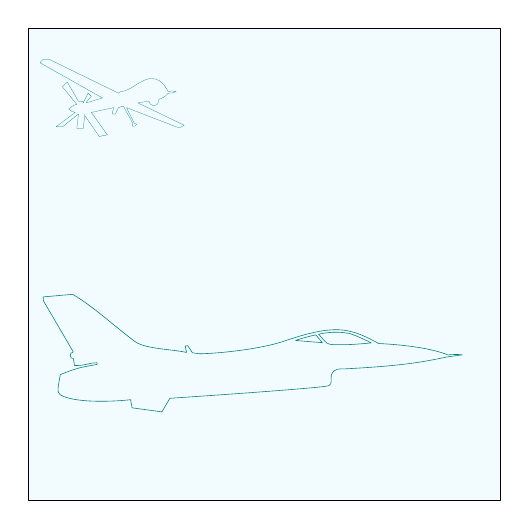
\begin{tikzpicture}[scale=1,line join=round,line cap=round,>=stealth]
		 \def\maybaytren{
		\tikz[yscale=-1]{ 
		\draw[teal] (0.8,24.9) --  (5.1,27.0) -- (5.2,26.9)
			 -- (5.3,26.9).. controls (5.8,26.8) and (6.1,26.5).. (6.5,26.3)..
			controls (7.5,25.7) and (8.0,26.5).. (8.2,26.9).. controls  (8.4,26.9) and
			(8.5,26.8)..  (8.7,26.9).. controls (8.6,27.0) and (8.4,27.0).. (8.2,
			27.0).. controls (8.1,27.1)  and (8.1,27.2).. (7.6,27.4).. controls (7.6,
			28.0) and (7.0,27.8).. (7.0,27.5)  -- (6.3,27.6) -- (9.2,29.0).. controls
			(9.1,29.1) and (8.9,29.2).. (8.7,29.1) -- (5.6,27.9) --  (6.1,28.9)..
			 controls (6.5,28.9) and (5.8,29.3).. (6.0,28.9) -- (5.4,27.8) -- (5.1,
			27.9) -- (4.9,28.3) -- (4.7,28.3) -- (4.8,27.9) -- (3.4,28.2) --  (4.4,
			29.6) -- (3.9,29.7) -- (3.0,28.4) --  (3.0,28.3) -- (2.9,29.2) -- (2.5,
			29.2) -- (2.6,28.3) -- (1.6,29.1) -- (1.2,29.1) -- (2.4,28.2).. controls 
			(2.2,28.2)  and (2.2,28.1).. (2.0,28.0).. controls (2.1,27.9) and (2.3,
			27.7).. (2.5,27.7) -- (1.6,26.6) -- (1.9,26.3) -- (2.6,27.5) -- (2.8, 
			27.5).. controls (2.9,27.5) and (2.9,27.5).. (2.9,27.6)  -- (3.2,27.0) --
			 (3.4,27.2).. controls (3.3,27.3) and (3.1,27.5).. (3.1,27.6) -- (4.1,
			27.3) -- (0.2,25.1).. controls (0.3,25.0) and (0.3,24.8).. (0.8,24.9) -- 
			cycle; 
			}} 
		\def\maybay#1{ 
		 \tikz[rotate=#1]{
		 \draw[teal]
			 (-7.14,0.31).. controls +(180:0) and +(209:0.1)..
			(-3.28,0.28).. controls +(21:0.1)  and +(253:0.1)..
			(-3.2,0.53).. controls  +(67:0.2) and +(180:0.1)..
			(-2.85,0.65).. controls +(358:1.2) and +(187:0.6).. 
			(-0.48,0.71).. controls +(10:0.1)  and +(0:0)..
			(0,0.74).. controls  +(166:0.1) and +(0:0.1)..
			(-0.35,0.77).. controls +(153:0.4) and  +(352:0.7)..
			(-1.99,1.19).. controls  +(147:0.3) and +(342:0.2)..
			(-2.62,1.53).. controls  +(159:0.4) and +(14:0.8)..
			 (-4.25,1.45).. controls +(194:0.6) and +(356:0.5)..
			(-6.33,1.32) -- (-6.5,1.36) -- (-6.6,1.54) -- (-6.66,1.54) -- 
			(-6.64,1.38).. controls +(163:0.4)  and +(319:0.3)..
			(-7.86,1.75).. controls +(138:0.7) and  +(324:0.6)..
			(-9.26,3.02) -- (-9.98,3.02).. controls +(233:0) and  +(124:0)..
			(-9.98,2.92).. controls +(297:0.1) and  +(115:0.3)..
			(-9.37,1.63)..  controls +(176:0.1) and +(180:0.1)..
			 (-9.38,1.47) -- (-9.37,1.3).. controls +(355:0.3) and +(175:0.2)..
			(-8.82,1.32) -- (-8.82,1.28).. controls +(185:0.4) and  +(18:0.4)..
			(-9.73,1.11)..  controls +(255:0.2) and +(148:0.1)..
			(-9.78,0.63)..  controls +(323:0.4) and +(182:0.4)..
			(-8.09,0.36)  -- (-8.07,0.16) -- (-7.36,0) -- cycle
			(-2.76,1.23).. controls +(175:0.3) and  +(323:0.1)..
			 (-3.24,1.31).. controls +(135:0.1) and +(307:0.1)..
			(-3.42,1.54).. controls +(0:0) and  +(163:0.4)..
			(-2.67,1.49).. controls +(339:0.2) and +(14:0).. 
			(-2.17,1.22).. controls +(198:0) and  +(356:0.2)..
			(-2.76,1.23)  -- cycle
			(-3.99,1.44).. controls  +(166:0) and +(186:0.2)..
			(-3.49,1.53).. controls +(306:0.1) and +(180:0).. 
			(-3.35,1.33).. controls  +(180:0) and +(349:0.2)..
			 (-3.99,1.44) -- cycle
			}} 
		\draw[fill=cyan!5]  (-3,-3) rectangle (3,3);
		\path (-3,-2) node[anchor=south west] (maybay)  {\resizebox{!}{1.5cm}{\maybay{5}}};
		\path (-3,1.5)  node[anchor=south west] (maybay) {\resizebox{!}{1cm}{\maybaytren}};
	\end{tikzpicture}
	} 
	 \noindent
	Trong khu vực hoạt động, có một trạm radar cảnh giới mặt đất của đối phương đặt tại $C(150;200;8)$. Radar  này có tầm quét hiệu dụng là một hình cầu $S$ tâm $C$ bán kính $R=6$ km. Để đảm bảo yếu tố bí mật và an toàn, toàn bộ đường bay của F-22 từ điểm xuất phát $A$ đến điểm đánh chặn $I$ (nơi F-22 gặp drone) phải nằm hoàn toàn bên ngoài khối cầu mở xác định bởi $S$ (có thể tiếp xúc với mặt cầu). Xác định thời điểm $t$ (tính bằng phút, làm tròn đến hàng đơn vị) sớm nhất có thể mà máy bay F-22 có thể đánh chặn thành công máy bay không người lái, biết rằng điều kiện về an toàn (tránh vùng radar) phải được đảm bảo.
	\shortans{13} 
	 \loigiai{
		 Gọi $I$ là điểm đánh chặn.\\
		Tại thời điểm $t$, F-22 gặp drone, do đó $I$ chính là vị trí của drone $D(t)$ $\Rightarrow$  $I=(500-20t; 500-15t; 5)$.\\
		Quãng đường F-22 bay được là $AI$.\\  Thời gian F-22 bay từ $A \to I$ là $t_{\mathrm{F-22}}=\dfrac{AI}{v_{\mathrm{F-22}}}=\dfrac{AI}{30}$.\\
		Để đánh chặn xảy ra  tại thời điểm $t$, thì $t=t_{\mathrm{F-22}} \Rightarrow AI=30t$.\\
		Với $A(0;0;10)$ và $I=(500-20t;  500-15t; 5)$ thì
		\allowdisplaybreaks 
		\begin{eqnarray*}
			&& AI^2=(500-20t)^2 + (500-15t)^2 +  5^2 \\
			&\Rightarrow& 900t^2=625t^2 -  35\,000t + 50\,0025 \\
			&\Leftrightarrow& t \approx  13.
		\end{eqnarray*}
		Do radar có tầm quét hiệu dung là một hình cầu  $S$ tâm $C$, bán kính $R=6$ km nên
		ta cần $AI$ phải  nằm hoàn toàn bên ngoài hoặc tiếp xúc với mặt cầu $S$.\\
		Ta có $\mathrm{d}(C,AI)=\dfrac{\left|\left[\overrightarrow{AC},\overrightarrow{AI}\right]\right|}{\left|\overrightarrow{AI}\right|}  \approx 6{,}0625\,\text{ km} > R=6$ km (thỏa mãn).\\
		Vậy thời điểm $t$ sớm nhất có thể mà máy bay F-22 có thể đánh chặn  thành công máy bay không người lái là $13$ giây.
	} 
\end{bt}

% nguồn: Phan2_Lop_12_Hinh_hoc_Chuong_5
\begin{bt}%[2H5V2-8]%[ma:0d221aba]
	Một kim tự tháp có các đỉnh $A(100;0;0)$, $B(100;100;0)$, $C(0;100;0)$, $D(0;0;0)$ và đỉnh $S(50;50;100)$. Từ mặt bên $BCS$ nhô ra một thanh $PQ$ thẳng đứng (là  một phần của cơ cấu nâng), trung điểm $T$ của thanh $PQ$ được đỡ bởi cột thẳng đứng $RT$. Biết $P(50;60;80)$, $Q(50;100;100)$. Tính chiều dài cột $TR$.
	\begin{center}
		\begin{tikzpicture}[line join = round,line cap=round,>=stealth,font=\footnotesize,scale=1]
				 \path
					 (0,0) coordinate (A)
					(4,0) coordinate (B) 
					(6,2) coordinate (C) 
					(2,2) coordinate (D) 
					(intersection of C--A and  B--D) coordinate (O)
					($(O)+(0,4)$)  coordinate (S)
					($(B)! 1/2  !(C)$) coordinate (B1)
					($(S)! 1/6 !(B1)$) coordinate (P) 
					($(S)+(2.3,0)$) coordinate  (Q)
					($(P)! 1/2 !(Q)$)  coordinate (T)
					($(S)!2/3!(B1)$) coordinate (R); 
				\draw  (A)--(B)--(C)--(D)--cycle;
				 \draw[->] (D)--++(0,4) node[left]{$z$};
				\draw[fill=gray!50] (S)--(A)--(B)--cycle (S)--(B)--(C)--cycle; 
				 \draw[red,line width=1.5] (P)--(Q);
				\draw[cyan,line width=1.5] (T)--(R); 
				 \draw[->] (A)--++(-0.5,-0.5) node[below]{$x$};
				\draw[->] (C)--++(0.5,0) node[below]{$y$}; 
				\foreach \p/\r in {A/-90,B/-90,C/45,S/90,P/-80,Q/0,T/90,R/-90} 
				\fill (\p) circle (1.2pt)  node[shift={(\r:3mm)}]{$\p$};
			\end{tikzpicture}
	\end{center}
	\shortans{50} 
	\loigiai{ 
		Xét  mặt phẳng $(BCS)$, ta có\\
		$\overrightarrow{BC} = (-100;0;0)$, $\overrightarrow{BS} = (-50;-50;100)$, $\overrightarrow{n}  = \left[\overrightarrow{BC},\overrightarrow{BS}\right] = (0;10\,000;5\,000) \sim (0;2;1)$.\\
		Suy ra phương trình tổng quát là $(BCS)\colon 2y + z - 200  = 0$.\\
		 Lại có $T$ là trung điểm của $PQ$ (gt).\\
		Do  đó $T(50;80;90)$.\\
		Mặt khác, cột $RT$ thẳng đứng (song song $Oz$) có phương trình $g\colon \heva{&x = 50 \\ &y = 80 \\ &z  = 90 + \lambda}$, $(\lambda \in \mathbb{R})$.\\
		Giao với $(BCS)\colon 2 \cdot 80 +  (90 + \lambda) - 200 = 0 \Rightarrow \lambda = -50$.\\
		Suy  ra $R(50;80;40)$.\\
		 Vậy $TR = 50$.
	} 
\end{bt}

% nguồn: Phan2_Lop_12_Hinh_hoc_Chuong_5
\begin{bt}%[2H5V2-8]%[ma:28c7a053]
	Một tàu ngầm bắt đầu lặn tại điểm $P(100;200;0)$ với vận tốc $11{,}1$ hải lý/giờ theo  hướng tới mục tiêu $Z(500;600;-80)$ cho đến khi đạt độ sâu $80$\,m. ($1$ hải lý/giờ sắp xỉ $1{,}852$\,km/h). Sau đó, tàu tiếp tục di chuyển ngang hướng theo vectơ $\overrightarrow{u}=(1;1;0)$ với vận tốc $11$ hải lý/giờ. Một quả cầu được thả đồng thời khi tàu ngầm bắt đầu lặn, từ tàu nghiên cứu $S(700;800;0)$ và rơi thẳng đứng xuống với vận tốc $0{,}5$\,m/s. Tính khoảng cách tàu ngầm với quả cầu khi tàu ngầm đi đến thẳng dưới $S$ (làm tròn kết quả đến hàng đơn vị).
	\begin{center}
		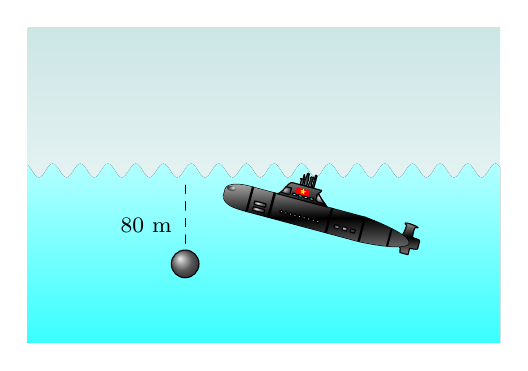
\begin{tikzpicture}[line cap=round,line join=round,>=stealth,font=\footnotesize]
				 \tikzset{taungam/.pic={
				\begin{scope}
					\draw[top color=black!30,bottom color=black!50,middle color=black] (1.11,0.98)..controls++(201:0.06) and++(282:0.08)..(1.02,1.41)..controls++(25:0.42) and++(121:0.07)..(0.53,1.44)..controls++(317:0.15)  and++(86:0.63)..(0.66,1)..controls++(246:0.06) and++(106:0.08)..(0.32,0.92)--(0.32,0.57).. controls++(312:0.07) and++(178:0.09)..(0.65,0.51)--(0.65,0.23)--(1,0.23)..controls++(73:0.15) and++(195:0.12)..(1.14,0.51);
					\def\a{(2.79,1.29)--(7.74,1.29)..controls++(1.38:0.93) and++(90:0.1)..(8.84,0.92)--(8.84,0.6)..controls++(249:0.37)  and++(0.6:0.53)..(7.74,0.23)--(2.79,0.23)..controls++(177:2.65) and++(186:2.81)..(2.79,1.29);}
					\draw \a 
					\path[top color=black!30,bottom color=black!50,middle color=black]  \a
					\draw[bottom color=black] (6.68,1.29)..controls++(168:0.26) and++(9:0.22)..(6.14,1.91)--(4.88,1.91)..controls++(258:0.23)  and++(39:1.08)..(4.47,1.29)--cycle;
					\draw[rounded corners=0.05mm,ball color=gray] (3.07,0.52)  rectangle (3.27,0.66)
						(3.42,0.52) rectangle (3.62,0.66) 
						(3.77,0.52) rectangle  (3.97,0.66);
					 \draw[ball color=gray] (6.37,1.68)--(6.14,1.68)--(6.14,1.43)--(6.17,1.39)--(6.21,1.38)--(6.54,1.39)--(6.46,1.50)--(6.40,1.62)--cycle;
					\draw[ball color=gray]  (4.95,1.72)--(5.02,1.72)--(5.02,1.48)--(5.01,1.45)--(4.98,1.42)--(4.95,1.40)--(4.91,1.39)--(4.59,1.39)--(4.67,1.45)--(4.76,1.53)--(4.86,1.62)--(4.92,1.68)--cycle;
					\draw[top color=red!30,bottom color=red!50,middle color=red]  (1.58,1.10)--(1.62,1.11)--(1.62,0.37)--(1.58,0.38)--cycle;
					\draw[top color=red!30,bottom  color=red!50,middle color=red] (2.79,1.29)--(2.79,0.24)--(2.84,0.24)--(2.84,1.29)--cycle;
					\draw[top color=red!30,bottom color=red!50,middle  color=red] (4.23,1.29)--(4.28,1.29)--(4.28,0.25)--(4.23,0.24)--cycle;
					\draw[top color=red!30,bottom color=red!50,middle color=red] (6.74,1.29)--(6.80,1.29)--(6.80,0.24)--(6.74,0.24)--cycle; 
					\draw[top  color=red!30,bottom color=red!50,middle color=red] (7.70,1.29)--(7.75,1.29)--(7.75,0.24)--(7.70,0.24)--cycle;
					\foreach \x  in{0,1,2,...,8}{\draw[ball color=gray] ({4.7+0.2*\x},0.6) circle (2pt);}
					 \draw[rounded corners=0.05mm,ball color=gray] (7,0.35) rectangle (7.5,0.5);
					\draw[rounded corners=0.05mm,ball color=gray] (7,0.6)  rectangle (7.5,0.75);
					\foreach \x in{0,1,2,3}{\draw[ball color=cyan]  (5.2+0.25*\x,1.45) ellipse ({0.1} and {0.05});}
					\shade[ball color= gray,shading  angle=-90] (8.6,1) ellipse ({0.2} and {0.1});
					\draw[left  color=gray,right color=black] (5.23,1.92)--(5.23,2.45)--(5.25,2.47)--(5.28,2.47)--(5.30,2.45)--(5.30,1.92)--cycle;
					\draw[left color=gray,right color=black] (5.35,1.92)--(5.35,2.06)--(5.37,2.06)--(5.37,2.27)--(5.35,2.27)--(5.35,2.33)--(5.36,2.33)--(5.36,2.35)--(5.46,2.35)--(5.46,2.33)--(5.47,2.33)--(5.47,2.27)--(5.46,2.27)--(5.46,2.06)--(5.47,2.06)--(5.48,1.92)--cycle; 
					 \draw[left color=gray,right color=black] (5.54,1.93)--(5.54,2.28)--(5.56,2.30)--(5.56,2.44)--(5.61,2.47)--(5.65,2.44)--(5.65,2.30)--(5.67,2.28)--(5.67,1.93)--cycle;
					 \draw[left color=gray,right color=black] (5.72,1.92)--(5.72,2.15)--(5.70,2.15)--(5.70,2.17)--(5.73,2.17)--(5.73,2.31)--(5.74,2.31)--(5.74,2.17)--(5.75,2.17)--(5.75,2.37)--(5.77,2.37)--(5.77,2.17)--(5.88,2.17)--(5.88,2.15)--(5.83,2.15)--(5.83,1.92)--cycle;
					\begin{scope}
						 \def\a{0.1}
						\fill[red] (5.35,1.51) rectangle (5.93,1.77); 
						\fill[yellow] (5.5,1.7) --++(0:\a)--++(72:\a)--++(-72:\a)--++(0:\a)--++(-144:\a)--++(-72:\a)--++(144:\a)--++(-144:\a)--++(72:\a)--++(144:\a); 
					\end{scope}
				\end{scope}
					}} 
				 \clip (0,0) rectangle (6,4);
				 \fill[top color=teal!20] (0,0) rectangle (6,4);
				\fill[decorate,decoration={snake},bottom  color=cyan,top color=cyan!30] (-1,-1)--++(90:3)--++(0:7)--(7,-1)--cycle;
				\pic[xscale=-1,scale=0.3,rotate=15] at  (5,1) {taungam};
				\draw[dashed] (2,2)--++(-90:1)  coordinate (A);
				 \draw[ball color=gray] (A) circle (5pt);
				\path (A)++(135:0.7) node {$80$ m}; 
			\end{tikzpicture}
	\end{center}
	\shortans{5} 
	 \loigiai{
		Ta  có $\overrightarrow{PZ}=(400;400;-80)$.\\
		Đoạn lặn $P\to Z$ (dừng ở độ sâu  $80$\,m) có phương trình $\heva{&x=100+400t\\& y=200+400t\\&z=0-80t},\,0\le t\le1$.\\
		Chuyển  động ngang từ $Z$ theo vectơ $\overrightarrow{u}=(1;1;0)$ có phương trình $\heva{&x=500+s\\ &y=600+s\\ &z=-80},\,s\ge0$.\\
		Quả cầu rơi thẳng đứng từ $S$ theo phương thẳng đứng với phương trình  $\heva{&x=700\\ &y=800\\&z=-0{,}5\tau},\,\tau\ge0$.\\
		Tàu đi đến thẳng dưới $S$ khi $x=700$ $y=800\Rightarrow  s=200$.\\
		Thời gian lặn  $P\to Z$ là $ t_1=\dfrac{|\overrightarrow{PZ}|}{11{,}1}=\dfrac{80\sqrt{51}}{5{,}7103}\approx100{,}05$\,s;\\
		Thời gian đi ngang tới dưới $S$ là  $ t_2=\dfrac{200\sqrt{2}}{11}=\dfrac{200\sqrt{2}}{5{,}6589}\approx49{,}98$\,s.\\
		 Lúc đó quả cầu có $z=-0{,}5(t_1+t_2)\approx-75$\,m, còn tàu ở $z=-80$\,m.\\
		Vậy khoảng cách  giữa tàu ngầm với quả cầu bằng $5$\,m.
	} 
\end{bt}

% nguồn: Phan2_Lop_12_Hinh_hoc_Chuong_5
\begin{bt}%[2H5V2-8]%[ma:ef99ef91]
	Một chiếc bàn gấp gọn đã được thiết lập hệ tọa  độ $Oxyz$. Điểm $A$ là chân bàn tiếp xúc với mặt đất thuộc đường thẳng $a\colon \heva{&x=-3+t\\&y=1+t\\&z=-2+4t}$ cắt mặt bàn $(P)\colon x+y-2z+6=0$ tại điểm $F$. Độ dài chân bàn $F A=40\sqrt 3\mathrm{~cm}$, khi đó độ cao của mặt bàn tính từ mặt đất là là bao nhiêu cm?
	\begin{center}
		\begin{tikzpicture}[line join=round,line cap=round,>=stealth]
				\draw[line width=4pt,orange!80!white] (-2.21,-1.23)--(-0.07,-2.76); 
				\draw[line  width=4pt,brown!60!black] (-1.55,-0.26)--(0.83,-1.5);
				\draw[line  width=5pt,brown!70!black] (1.37,0.82) -- (-0.46,-3.73);
				\draw[line width=5pt,brown!90!black] (-2.5,-2) -- (-1.08,1.76); 
				\draw[line width=5pt,brown!70!black] (0,0) --  (1.21,-2.18);
				\draw[line width=5pt,brown!70!black] (-2.74,1.12) -- (-1.02,-0.88); 
				 \draw[fill=orange!80!gray](0,0)--(-3.26,1.37)--(-1.02,2.24)--(2.3,1.62)--cycle;
				\draw[fill=orange!70!white](0,0)--(0,-0.15)--(-3.26,1.22)--(-3.26,1.37)--cycle; 
				 \draw[fill=orange!70!black](0,0)--(0,-0.15)--(2.3,1.47)--(2.3,1.62)--cycle;
				\coordinate  (F) at (0,0);
				\coordinate  (A) at (1.21,-2.18);
				\coordinate (f) at  (2.3,1.62);
				\coordinate (ff)  at ($(F)!1.4!(f)$);
				\coordinate (a) at  ($(F)!1.4!(A)$);
				\draw pic[draw,angle radius=0.5cm,red]{angle=A--F--f}; 
				\draw[line width=3pt,red]  (ff)--(F)--(a);
				\foreach  \i/\g in {F/90,A/200}{\draw[fill=red](\i) circle (1.5pt)
					 ($(\i)+(\g:3mm)$) node[scale=1]{$\i$};}
				\draw  ($(a)+(-135:3mm)$) node[scale=1]{$a$};
			\end{tikzpicture}
	\end{center}
	\shortans{40} 
	 \loigiai{
		\begin{center}
			\begin{tikzpicture}[line join=round,line cap=round,>=stealth]
					\draw[line width=4pt,orange!80!white]  (-2.21,-1.23)--(-0.07,-2.76);
					\draw[line width=4pt,brown!60!black] (-1.55,-0.26)--(0.83,-1.5); 
					\draw[line width=5pt,brown!70!black] (1.37,0.82) --  (-0.46,-3.73);
					\draw[line width=5pt,brown!90!black] (-2.5,-2) -- (-1.08,1.76); 
					\draw[line width=5pt,brown!70!black] (0,0) --  (1.21,-2.18);
					\draw[line  width=5pt,brown!70!black] (-2.74,1.12) -- (-1.02,-0.88);
					\draw[fill=orange!80!gray](0,0)--(-3.26,1.37)--(-1.02,2.24)--(2.3,1.62)--cycle; 
					\draw[fill=orange!70!white](0,0)--(0,-0.15)--(-3.26,1.22)--(-3.26,1.37)--cycle; 
					 \draw[fill=orange!70!black](0,0)--(0,-0.15)--(2.3,1.47)--(2.3,1.62)--cycle;
					\coordinate (F)  at (0,0);
					\coordinate  (A) at (1.21,-2.18);
					 \coordinate (f) at (2.3,1.62);
					\coordinate  (H) at ($(F)!0.6!(f)$);
					 \coordinate (ff) at ($(F)!1.4!(f)$);
					 \coordinate (a) at ($(F)!1.4!(A)$);
					\draw pic[draw,angle  radius=0.5cm,red]{angle=A--F--f};
					\draw[line width=3pt,red] (ff)--(F)--(a); 
					 \foreach \i/\g in {F/90,H/90,A/200}{\draw[fill=red](\i) circle (1.5pt)
						($(\i)+(\g:3mm)$) node[scale=1]{$\i$};} 
					 \draw ($(a)+(-135:3mm)$) node[scale=1]{$a$};
				\end{tikzpicture}
		\end{center}
		Đường thẳng  $a\colon \heva{&x=-3+t\\&y=1+t\\&z=-2+4t}$ có vectơ chỉ phương $\overrightarrow{u}=(1;1;4)$.\\
		Mặt phẳng $(P)\colon x+y-2z+6=0$ có vectơ pháp tuyến  $\overrightarrow{n}=(1;1;-2)$.\\
		$\sin  \Big(a,(P)\Big)=\left|\cos \Big(\overrightarrow{u},\overrightarrow{n}\Big)\right|=\dfrac{\left|\overrightarrow{u}\cdot \overrightarrow{n}\right|}{\left|\overrightarrow{u}\right| \cdot \left|\overrightarrow{n}\right|}=\sqrt{\dfrac{1}{3}}=\sin \varphi$.\\
		Độ cao của mặt bàn tính từ mặt đất là khoảng cách từ  chân bàn $A$ đến mặt phẳng $(P)$.\\
		Suy ra $\mathrm{d}\Big(A,(P)\Big)=AH=FA\cdot  \sin \varphi=40\sqrt 3\cdot \sqrt{\dfrac{1}{3}}=40$ cm.
	 }
\end{bt}

% nguồn: Phan2_Lop_12_Hinh_hoc_Chuong_5
\begin{bt}%[2H5C2-8]%[ma:9ec0d92d]
	\immini{Trên mặt đất phẳng, người ta dựng một cây cột thẳng cao $6$ m vuông góc với mặt đất, có chân cột đặt tại ví trí $O$ trên mặt đất. Tại một thời điểm, dưới ánh nắng mặt trời, bóng của đỉnh cột dưới mặt đất cách chân cột $4$ m về hướng S$60^\circ$E (hướng tạo với hướng nam góc $60^\circ$ tạo với hướng đông góc $30^\circ$) (Hình $5$.$32$). Chọn hệ trục $Oxyz$ có gốc tọa độ là $O$, tia $Ox$ chỉ hướng nam, tia $Oy$ chỉ hướng đông, tia $Oz$ chứa cây cột, đơn vị đo là mét. Phương trình đường thẳng chứa tia nắng mặt trời đi qua đỉnh cột tại thời điểm đang xét có phương trình $\dfrac{x-x_0}{a} = \dfrac{y-y_0}{\sqrt{3}} = \dfrac{z-z_0}{c}$. Tính $x_0+a+c$.} 
	{ 
	\begin{tikzpicture}[scale=1,font=\footnotesize,line join=round,line cap=round,>=stealth]
			\coordinate  (O) at (0,0);
			\coordinate (S) at  (-1,-1);
			 \coordinate (E) at (2,0);
			\coordinate (A)  at (0,1);
			 \coordinate (A') at (1,-0.5);
			\draw[->] (O)--(E) node[below] {$y$} node[above] {$E$}; 
			\draw[->]  (O)--(S) node[right] {$x$} node[left] {$S$};
			\draw[->] (O)-((0,2) node[right] {$z$}; 
			\foreach  \x/\y in {A/0,A'/-90,O/180}{
				 \draw (\x) circle (1pt)
				($(\x)+(\y:3mm)$) node{$\x$}; 
			 }
			\foreach \x/\y/\z in {A'/O/E}{ 
				\path  pic[draw,angle radius=10pt,pic text=$30^{\circ}$,
				pic text  options={shift={(20pt,-4pt)}}]{angle= \x--\y--\z};}
			\foreach  \x/\y/\z in {S/O/A'}{
				\path  pic[draw,angle radius=7pt,pic text=$60^{\circ}$,
				 pic text options={shift={(0,-7pt)}}]{angle= \x--\y--\z};}
			\draw  (O)--(A');
		\end{tikzpicture}
	\par 
	\textit{Hình $5$.$32$}} 
	\shortans{0} 
	 \loigiai{
		Theo cách chọn hệ  trục tọa độ, ta có:\\
		- Đỉnh cột là điểm  $A(0;0;6)$.\\
		- Bóng của đỉnh cột trên mặt đất là điểm $A'$. Vì $A'$ cách $O$ một khoảng $4$  m về hướng S$60^\circ$E, ta có $x_A' = 4\cos 60^\circ = 2$ và $y_A' = 4\sin 60^\circ = 2\sqrt{3}$. Vậy $A'(2;2\sqrt{3};0)$.\\
		Đường thẳng chứa tia nắng  đi qua hai điểm $A$ và $A'$ nên có một véc-tơ chỉ phương là $\overrightarrow{HP}=(0-2;0-2\sqrt{3};6-0)=(-2;-2\sqrt{3};6)$.\\
		Ta  chọn một véc-tơ chỉ phương khác cùng phương là $\overrightarrow{u}=(1;\sqrt{3};-3)$.\\
		Phương trình đường thẳng đi qua  $A'(2;2\sqrt{3};0)$ là $\dfrac{x-2}{1}=\dfrac{y-2\sqrt{3}}{\sqrt{3}}=\dfrac{z}{-3}$.\\
		Vậy $x_0+a+c=2+1+(-3)=0$. 
	} 
\end{bt}

% nguồn: Phan2_Lop_12_Hinh_hoc_Chuong_5
\begin{bt}%[2H5C2-8]%[ma:762981ea]
	Khi khắc phục hậu quả của thiên tai, bão lũ, một trong những  giải pháp nhằm tiếp tế hàng cứu trợ đến những nơi khó tiếp cận là sử dụng flycam để xác định vị trí chính xác của người cần cứu trợ, sau đó sử dụng drone để vận chuyển các vật dụng thiết yếu thả xuống cho người này, giúp họ có thể cầm cự trong khi chờ đợi lực lượng cứu hộ đến nơi. Hai chiếc drone làm nhiệm vụ chuyển hàng cứu trợ bay lên từ cùng một địa điểm. Chiếc thứ nhất bay đến điểm cách điểm xuất phát $2{,}5$\,km về phía nam và $1{,}5$\,km về phía đông, đồng thời cách mặt đất $60$\,m. Chiếc thứ hai bay đến điểm cách điểm xuất phát $3$\,km về phía bắc và $2{,}5$\,km về phía tây, đồng thời cách mặt đất $40$\,m. Trong không gian, xét hệ tọa độ $Oxyz$ với gốc tọa độ $O$ đặt tại điểm xuất phát của hai chiếc drone, mặt phẳng $(Oxy)$ trùng với mặt đất (được coi là mặt phẳng). Giả sử trong trường hợp khẩn cấp cần tìm một vị trí trên mặt đất để tiếp nhiên liệu và các vật dụng cứu trợ cho hai drone sao cho tổng khoảng cách từ vị trí tiếp nhiên liệu tới hai drone nhỏ nhất. Vị trí cần tìm cách gốc tọa độ $a$\,km theo hướng bắc và $b$\,km theo hướng tây. Khi đó $a+b$ bằng bao nhiêu?
	\begin{center}
		\begin{tikzpicture}
				\path (0,0)  node[above] (O){
				\resizebox{!}{2cm}{\begin{tikzpicture}
					\path[fill=blue,line width=0.1cm] (2.51,2.07).. controls (1.39,2.12) and (1.35,2.35).. (1.37,2.58).. controls (0.3,2.07) and (0.69,0.97).. (0.56,0.07) -- (0.01,0.07) -- (0.0,2.69).. controls (-0.46,3.17) and (-1.53,2.91).. (-2.33,2.98) -- (-2.33,3.34) -- (-1.97,3.35) -- (-1.93,3.63) -- (-1.74,3.59) -- (-1.99,3.8).. controls (-2.8,3.71) and (-3.58,3.75).. (-4.2,3.89).. controls (-3.46,4.09) and (-2.71,4.09).. (-1.96,4.1).. controls (-1.96,4.1) and (-1.74,4.32).. (-1.48,4.31).. controls (-1.22,4.29) and (-1.01,4.12).. (-1.01,4.12).. controls (-0.31,4.13) and (0.44,4.2)..  (1.04,4.06).. controls (0.52,3.85) and (-0.26,3.84).. (-1.04,3.82) -- (-1.21,3.6) -- (-1.01,3.6) -- (-0.99,3.34).. controls (0.16,3.56) and (1.27,3.85).. (2.53,3.84).. controls (3.94,3.82) and (4.95,3.51).. (6.12,3.31) -- (6.12,3.6) -- (6.35,3.59) -- (6.05,3.84).. controls (4.92,3.85) and (4.31,3.93).. (3.92,4.05).. controls (4.51,4.17) and (5.31,4.14).. (6.09,4.12).. controls (6.09,4.12) and (6.43,4.37).. (6.61,4.36).. controls (6.79,4.36) and (7.03,4.09).. (7.03,4.09).. controls (7.75,4.03) and (8.53,4.1).. (9.19,3.87).. controls (8.5,3.68) and (7.76,3.79).. (7.04,3.77) -- (6.84,3.57) -- (7.03,3.6) -- (7.04,3.35) -- (7.39,3.35) -- (7.39,2.98).. controls (6.59,2.91) and (5.45,3.04).. (5.07,2.74) -- (5.05,0.06) -- (4.46,0.07).. controls (4.33,0.96) and (4.77,2.14).. (3.74,2.58).. controls (3.73,2.18) and (3.06,2.01).. (2.51,2.07) -- cycle;
				\end{tikzpicture}
		 }};
		 \path (5,2) node[above] (A){
		\resizebox{!}{1cm}{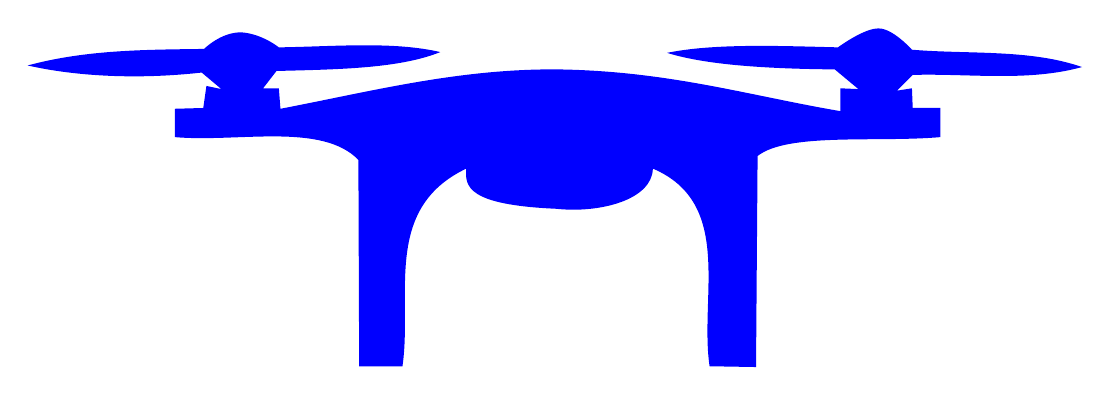
\begin{tikzpicture}
		\path[fill=blue,line width=0.1cm] (2.51,2.07).. controls (1.39,2.12) and (1.35,2.35).. (1.37,2.58).. controls (0.3,2.07) and (0.69,0.97).. (0.56,0.07) -- (0.01,0.07) -- (0.0,2.69).. controls (-0.46,3.17) and (-1.53,2.91).. (-2.33,2.98) -- (-2.33,3.34) -- (-1.97,3.35) -- (-1.93,3.63) -- (-1.74,3.59) -- (-1.99,3.8).. controls (-2.8,3.71) and (-3.58,3.75).. (-4.2,3.89).. controls (-3.46,4.09) and (-2.71,4.09).. (-1.96,4.1).. controls (-1.96,4.1) and (-1.74,4.32).. (-1.48,4.31).. controls (-1.22,4.29) and (-1.01,4.12).. (-1.01,4.12).. controls (-0.31,4.13) and (0.44,4.2).. (1.04,4.06).. controls (0.52,3.85) and (-0.26,3.84).. (-1.04,3.82) -- (-1.21,3.6) -- (-1.01,3.6) -- (-0.99,3.34).. controls (0.16,3.56) and (1.27,3.85).. (2.53,3.84).. controls (3.94,3.82) and (4.95,3.51).. (6.12,3.31) -- (6.12,3.6) -- (6.35,3.59) -- (6.05,3.84).. controls (4.92,3.85) and (4.31,3.93).. (3.92,4.05).. controls (4.51,4.17) and (5.31,4.14).. (6.09,4.12).. controls (6.09,4.12) and (6.43,4.37).. (6.61,4.36).. controls (6.79,4.36) and (7.03,4.09).. (7.03,4.09).. controls (7.75,4.03) and (8.53,4.1).. (9.19,3.87).. controls (8.5,3.68) and (7.76,3.79).. (7.04,3.77) -- (6.84,3.57) -- (7.03,3.6) -- (7.04,3.35) -- (7.39,3.35) -- (7.39,2.98).. controls (6.59,2.91) and (5.45,3.04)..  (5.07,2.74) -- (5.05,0.06) -- (4.46,0.07).. controls (4.33,0.96) and (4.77,2.14).. (3.74,2.58).. controls (3.73,2.18) and (3.06,2.01).. (2.51,2.07) -- cycle;
	\end{tikzpicture}
		}}; 
	\end{tikzpicture}
\end{center}
\shortans{1,7} 
 \loigiai{
	 Ta có $60$\,(m)$=0{,}06$\,(km); $40$\,(m)$=0{,}04$\,(km).\\
	Chọn hệ trục toạ độ $Oxyz$ với gốc $O$ đặt tại điểm xuất phát  của hai drone, mặt phẳng $(Oxy)$ trùng với mặt đất, trục $Ox$ có hướng trùng với hướng nam, trục $Oy$ có hướng trùng với hướng đông, trục $Oz$ vuông góc với mặt đất hướng lên bầu trời, đơn vị trên mỗi trục tính theo\,$km$.
	\begin{center}
		\begin{tikzpicture} [line join=round]
				\def\khinhkicauden{ 
			\begin{tikzpicture}
					\def\than{(-0.16,0) coordinate (At) -- (0.23,0) coordinate (Bt).. controls (0.23,-0.01) and (2.29,2.19).. (2.52,3.0).. controls (2.75,3.82) and (2.83,4.31).. (2.5,4.82).. controls (2.04,5.53) and (1.03,5.86).. (0.18,5.88)..  controls (-0.7,5.9) and (-1.76,5.59).. (-2.28,4.87).. controls (-2.62,4.4) and (-2.55,3.69).. (-2.39,3.13).. controls (-2.04,1.9) and (-0.16,-0.02).. (-0.16,-0.02) -- cycle}
					\def\cabin{(-0.16,-0.4) coordinate (Ct) -- (0.23,-0.4) coordinate (Dt)..  controls (0.23,-0.41) and (0.38,-0.5).. (0.38,-0.61).. controls (0.38,-0.72) and (0.22,-0.88).. (0.08,-0.88).. controls (-0.06,-0.88) and (-0.24,-0.72).. (-0.23,-0.61).. controls (-0.23,-0.49) and (-0.16,-0.42).. cycle}
					 \path \than\cabin;
					\draw[shorten <=-5pt,shorten >=-5pt] (At)--(Ct) 
						(Bt)--(Dt); 
					 \path[ball color=red] \than;
					\path[ball  color=black] \cabin;
					\begin{scope}
						 \clip \than;
						 \path[fill=green!55!black]
						(-0.5,0).. controls (-1.2,1.2) and (-3.1,4.2).. (-0.5,5.8).. controls (-0.3,5.8) and  (-0.3,0).. (-0.5,0) -- cycle;
						\path[fill=green!55!black] 
						(0.5,0).. controls  (1.2,1.2) and (3.1,4.2).. (0.5,5.8).. controls (0.3,5.8) and (0.3,0).. (0.5,0) -- cycle;
					\end{scope}
				\end{tikzpicture}
	 }
	\coordinate  (O) at (0,0,0);
	 \draw[->] (0,0,0) -- (0,0,4.5) node[above left] {$x$};
	\draw[->] (0,0,0) -- (4.5,0,0)  node[below, yshift=-3pt] {$y$};
	 \draw[->] (0,0,0) -- (0,3.5,0) node[left] {$z$};
	\draw[dashed] (0,0,-4.5) -- (0,0,0) (-3.5,0,0) -- (0,0,0); 
	\foreach  \t/\g in {O/280}{
	\fill  (\t) circle (0.2pt) node[shift={(\g:10pt)}]{$\t$};
	 }
	\draw[dashed] (3,0,3) -- (3,0,0)  (3,0,3) -- (0,0,3) (3,2,3) -- (0,2,0)(-3,0,-2) -- (-3,0,0) (-3,0,-2) -- (0,0,-2) (-2.65,2,-1) -- (0,1.2,0);
	\fill  (3,2,3) circle (1.5pt);
	\draw[dashed] (-2.65,2,-1) -- (-3,0,-2)  (3,2,3) -- (3,0,3);
	\path (3,2,3) node[above]{ 
	\resizebox{!}{0.4cm}{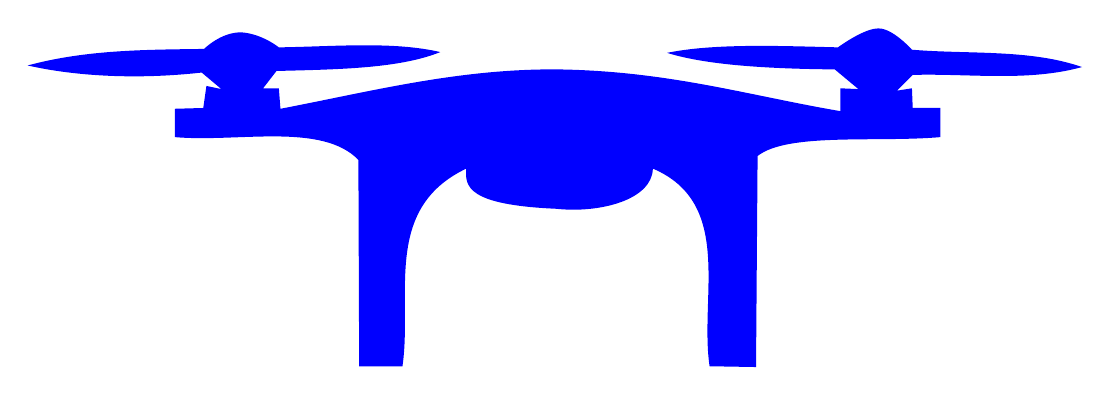
\begin{tikzpicture}
		\path[fill=blue,line width=0.1cm] (2.51,2.07).. controls (1.39,2.12) and (1.35,2.35).. (1.37,2.58).. controls (0.3,2.07) and (0.69,0.97).. (0.56,0.07) -- (0.01,0.07) -- (0.0,2.69).. controls (-0.46,3.17) and (-1.53,2.91).. (-2.33,2.98) -- (-2.33,3.34) -- (-1.97,3.35) -- (-1.93,3.63) -- (-1.74,3.59) -- (-1.99,3.8).. controls (-2.8,3.71) and (-3.58,3.75).. (-4.2,3.89).. controls (-3.46,4.09) and (-2.71,4.09).. (-1.96,4.1).. controls (-1.96,4.1) and (-1.74,4.32).. (-1.48,4.31).. controls (-1.22,4.29) and (-1.01,4.12).. (-1.01,4.12).. controls (-0.31,4.13) and (0.44,4.2).. (1.04,4.06).. controls (0.52,3.85) and (-0.26,3.84).. (-1.04,3.82) -- (-1.21,3.6) -- (-1.01,3.6) -- (-0.99,3.34).. controls (0.16,3.56) and (1.27,3.85).. (2.53,3.84).. controls (3.94,3.82) and (4.95,3.51).. (6.12,3.31) -- (6.12,3.6) -- (6.35,3.59) -- (6.05,3.84).. controls (4.92,3.85) and (4.31,3.93).. (3.92,4.05).. controls (4.51,4.17) and (5.31,4.14).. (6.09,4.12).. controls (6.09,4.12) and (6.43,4.37).. (6.61,4.36).. controls (6.79,4.36) and (7.03,4.09).. (7.03,4.09).. controls (7.75,4.03) and (8.53,4.1).. (9.19,3.87).. controls (8.5,3.68) and (7.76,3.79).. (7.04,3.77) -- (6.84,3.57) -- (7.03,3.6) --  (7.04,3.35) -- (7.39,3.35) -- (7.39,2.98).. controls (6.59,2.91) and (5.45,3.04).. (5.07,2.74) -- (5.05,0.06) -- (4.46,0.07).. controls (4.33,0.96) and (4.77,2.14).. (3.74,2.58).. controls (3.73,2.18) and (3.06,2.01).. (2.51,2.07) -- cycle;
	\end{tikzpicture}
	} }; 
	\fill (-2.65,2,-1)  circle (1.5pt);
	 \path (-2.65,2,-1) node[above]{
	\resizebox{!}{0.3cm}{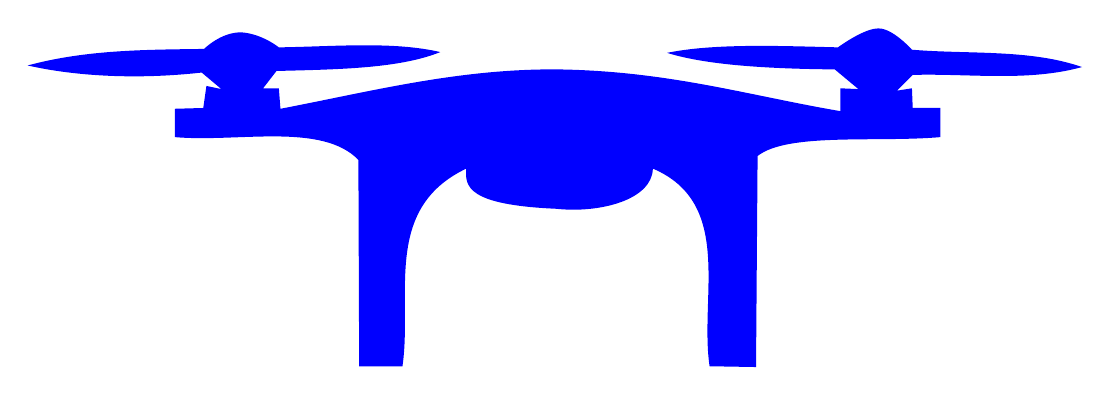
\begin{tikzpicture}
		\path[fill=blue,line width=0.1cm] (2.51,2.07).. controls (1.39,2.12) and (1.35,2.35).. (1.37,2.58).. controls (0.3,2.07) and (0.69,0.97).. (0.56,0.07) -- (0.01,0.07) -- (0.0,2.69).. controls (-0.46,3.17) and (-1.53,2.91).. (-2.33,2.98) -- (-2.33,3.34) -- (-1.97,3.35) -- (-1.93,3.63) -- (-1.74,3.59) -- (-1.99,3.8).. controls (-2.8,3.71) and (-3.58,3.75).. (-4.2,3.89).. controls (-3.46,4.09) and (-2.71,4.09).. (-1.96,4.1).. controls (-1.96,4.1) and (-1.74,4.32).. (-1.48,4.31).. controls (-1.22,4.29) and  (-1.01,4.12).. (-1.01,4.12).. controls (-0.31,4.13) and (0.44,4.2).. (1.04,4.06).. controls (0.52,3.85) and (-0.26,3.84).. (-1.04,3.82) -- (-1.21,3.6) -- (-1.01,3.6) -- (-0.99,3.34).. controls (0.16,3.56) and (1.27,3.85).. (2.53,3.84).. controls (3.94,3.82) and (4.95,3.51).. (6.12,3.31) -- (6.12,3.6) -- (6.35,3.59) -- (6.05,3.84).. controls (4.92,3.85) and (4.31,3.93).. (3.92,4.05).. controls (4.51,4.17) and (5.31,4.14).. (6.09,4.12).. controls (6.09,4.12) and (6.43,4.37).. (6.61,4.36).. controls (6.79,4.36) and (7.03,4.09).. (7.03,4.09).. controls (7.75,4.03) and (8.53,4.1).. (9.19,3.87).. controls (8.5,3.68) and (7.76,3.79).. (7.04,3.77) -- (6.84,3.57) -- (7.03,3.6) -- (7.04,3.35) -- (7.39,3.35) -- (7.39,2.98).. controls (6.59,2.91) and (5.45,3.04).. (5.07,2.74) -- (5.05,0.06) -- (4.46,0.07).. controls (4.33,0.96) and (4.77,2.14).. (3.74,2.58).. controls (3.73,2.18) and (3.06,2.01).. (2.51,2.07) -- cycle;
	\end{tikzpicture}
	}  };
	\node [above  right] at (3,2,3) {A};
	\node  [below left] at (-2.65,2,-1) {B};
	\node[above left] at (4.5,0,0) {Đ}; 
	\node[below] at (0,0,4.5) {N}; 
	\node[above right] at  (-3.5,0,0) {T};
\end{tikzpicture}
\end{center}
 Chiếc drone thứ nhất bay đến điểm $A(2{,}5;1{,}5;0{,}06)$, chiếc drone thứ hai bay đến điểm $B(-3;-2{,}5;0{,}04)$.\\
Gọi $C(x;y;0)$ là vị trí trên mặt đất để tiếp nhiên  liệu và các vật dụng.\\
Điểm đối xứng với $A$ qua mặt  phẳng $(Oxy)$ là $A'(2{,}5;1{,}5;-0{,}06)$.\\
 Khi đó $AC+CB=A'C+CB$.\\
Vì $A'$, $C$, $B$ khác phía so với $(Oxy)$ nên $A'C+CB$ nhỏ nhất khi $A'$, $C$, $B$ thẳng hàng.\\ 
Suy ra  $C=A'B\cap(Oxy)$.\\
Ta có $\overrightarrow{BA'}=(5{,}5;4;-0{,}1)$.\\ 
Phương trình  đường thẳng $BA'\colon\heva{&x=-3+5{,}5t\\&y=-2{,}5+4t\\&z=0{,}04-0{,}1t.}$\\
Phương  trình mặt phẳng $(Oxy)\colon z=0$.\\
Giao điểm của $A'B$ với  $(Oxy)$ là nghiệm của hệ
 $\heva{&x=-3+5{,}5t \\
&y=-2{,}5+4t \\ 
 &z=0{,}04-0{,}1t \\
&z=0}\Rightarrow 
\heva{&t=\dfrac{2}{5}  \\
&x=-\dfrac{4}{5}  \\
 &y=-\dfrac{9}{10} \\
&z=0} \Rightarrow 
 C\left(-\dfrac{4}{5};-\dfrac{9}{10};0\right)$.\\
Suy ra $a=-\dfrac{4}{5}$;  $b=-\dfrac{9}{10}$.\\
 Vậy $a+b=-\dfrac{17}{10}=-1{,}7$.
 }
\end{bt}


%%%%%%%%%%%%%%%% TỰ LUẬN %%%%%%%%%%%%%%%%

% nguồn: Phan2_Lop_12_Hinh_hoc_Chuong_5
\begin{bt}%[2H5H2-8]%[ma:2e65f097]
	Trên một sân khấu mô phỏng với hệ trục $Oxyz$, có hai tia sáng dọc theo hai đường thẳng có phương trình lần lượt là $d\colon \dfrac{x+3}{2}=\dfrac{y+2}{3}=\dfrac{z-6}{4}$ và $d'\colon \heva{&x=5+t' \\& y=-1-4  t'\\&z=20+t'}\,(t' \in \mathbb{R})$.\\
	Hỏi hai tia sáng giao nhau tại điểm có toạ độ  nào?
	\loigiai{ 
		Phương trình tham số của đường thẳng $d$ là $\heva{&x=-3+2t  \\ &y=-2+3 t \\ &z=6+4 t}\,(t \in \mathbb{R})$.\\
		 Xét phương trình hai ẩn $t$, $t'$ sau $\heva{&-3+2t=5+t'&\quad (1)\\&-2+3 t=-1-4t'&\quad (2) \\ &6+4 t=20+t'.&\quad (3)}$\\
		 Giải hệ phương trình $(1)$ và $(2)$ ta được $\heva{&t=3 \\&t'=-2.}$ thoả mãn (3).\\
		Thay $t=3$ vào phương trình tham số của đường thẳng $d$ ta có $\heva{&x=-3+2  \cdot 3 =3\\& y=-2+3\cdot 3=7 \\& z=6+4\cdot 3=18.}$\\
		Vậy toạ độ giao điểm của hai tia sáng là  $(3;7;18)$.
	 }
\end{bt}

% nguồn: Ok_TuanLuan_Toan11_Lan2
\begin{ex}%[2H5V2-8]%[ma:96f9afac]
	Một kĩ sư xây dựng thiết kế khung một ngôi nhà trong không gian $Oxyz$ như hình dưới đây nhờ một phần mềm  đồ hoạ máy tính.
	\begin{center}
		 \tdplotsetmaincoords{80}{100}
		\begin{tikzpicture}[tdplot_main_coords]
				 \coordinate (O) at (0,0,0);
				\coordinate (A)  at (8,0,0);
				\coordinate (B) at (8,6,0); 
				\coordinate (C)  at (0,6,0);
				\coordinate  (D) at (0,0,4);
				\coordinate (E) at (8,0,4); 
				 \coordinate (H) at (0,6,4);
				 \coordinate (N) at (0,3,6);
				\coordinate (M)  at (8,3,6);
				\draw[->] (A) --  (10,0,0) node[anchor=north east]{$x$};
				\draw[->] (C) -- (0,7,0)  node[above]{$y$};
				\draw[->]  (D) -- (0,0,7) node[anchor=south]{$z$};
				\draw (C) -- (B)  -- (A);
				\draw[dashed] (C) -- (O) --  (D);
				\draw (A)  -- (E);
				\draw (C) --  (H);
				\draw (D) --  (E);
				 \draw (E) -- (8,6,4) -- (B);
				\draw (8,6,4) --  (H);
				\draw[dashed] (H) -- (D) -- (O)  -- (A);
				\draw[very thick]  (D) -- (E);
				\draw[very thick]  (E) -- (M) -- (8,6,4);
				\draw[very thick] (M)  -- (N) -- (H);
				\draw[very thick] (N) -- (D); 
				 \node[below right] at (O) {$O (0; 0; 0)$};
				\node[below right] at (C) {$C (0; 4; 0)$}; 
				 \node[below] at (B) {$B$};
				\node[above  left] at (A) {$A (6; 0; 0)$};
				\node[above left]  at (D) {$D (0; 0; 4)$};
				 \node[above left] at (E) {$E (6; 0; 4)$};
				 \node[above right] at (H) {$H$};
				 \node[above] at (N) {$N (0; 2; 6)$};
				\node[right] at  (M) {$M (6; 2; 6)$};
				\node[right] at  (B) {};
				\node[right] at (C) {}; 
				\node[right] at (D) {}; 
				\node[right]  at (E) {};
				\node[right] at (H) {}; 
			\end{tikzpicture}
	\end{center}
	\begin{enumerate}
		\item[a)] Viết phương trình mặt phẳng  mái nhà $(DEMN)$.
		\item[b)] Tính khoảng cách từ điểm $B$ đến mái nhà $(DEMN)$. 
	\end{enumerate}
	 \loigiai{
		\begin{enumerate}
			 \item
			Mặt  phẳng $(DEMN)$ có 2 vectơ chỉ phương
			$$ 
			\vec{DE} = (6;0;0),\, \vec{DN} = (0;2;2) 
			\Rightarrow \left[\vec{DE}, \vec{DN}\right] = (0;  -12; 12)
			 \Rightarrow \vec{n} = -\dfrac{1}{12}(0; -12; 12) = (0;1;-1).
			$$ 
			 Phương trình mặt phẳng $(DEMN)$ đi qua điểm $D(0;0;4)$, nhận $\vec{n} = (0;1;-1)$ làm véc-tơ pháp tuyến nên có dạng
			 $$
			0(x - 0) + 1(y - 0) -1(z - 4) = 0 \Rightarrow y - z +  4 = 0.
			$$ 
			\item Ta có 
			 $$
			\mathrm{d}\left(B, (DEMN)\right) = \dfrac{\left|4 - 0 + 4\right|}{\sqrt{0^2 + 1^2 + (-1)^2}} = \dfrac{8}{\sqrt{2}}  = 4\sqrt{2}.
			 $$
		\end{enumerate}
	 }
\end{ex}

% nguồn: Ok_TuanLuan_Toan11_Lan2
\begin{ex}%[2H5V2-8]%[ma:c38efa3f]
	Người ta muốn dựng một cột ăngten trên một sườn đồi. Ăngten được dựng thẳng đứng trong không gian $Oxyz$ với độ dài đơn vị trên mỗi trục bằng $1$m. Gọi $O$ là gốc cột, $A$ là  điểm buộc dây cáp vào cột ăngten và $M, N$ là hai điểm neo dây cáp xuống mặt sườn đồi (hình vẽ).
	\begin{center}
		\begin{tikzpicture}[line cap=round,line join=round]
				\path[fill=green!30!yellow!50] (0.55,0).. controls +(51:1) and  +(-175:0.7).. (2.8,1.67).. controls +(4:1.6) and +(0:0).. (5.03,0);
				\path[fill=green!70!black] (0,0).. controls +(63:0.1) and +(179:0.9).. (1.95,1.25).. controls +(0:1.2) and +(0:0)..  (4.4,0);
				 \path[fill=green!85!black] (1.36,0).. controls +(41:1.9) and +(-179:1.4).. (4.98,1.97).. controls +(1:1.5) and +(129:1.1).. (8.33,0.02);
				 \path[fill=green] (0.75,0).. controls +(42:0.7) and +(-178:0.6).. (2.48,0.83).. controls +(2:0.7) and +(132:0.8).. (4.19,0);
				\draw[line width=2pt] (7.64,0.47) coordinate  (O)--+(0,2.5) coordinate (B);
				\draw[green!30]  (O)--(B);
				\draw[semithick] (4.91,1.43) coordinate (M) -- ($(O)!0.5!(B)$) coordinate (A) 
					-- (4.21,0.72) coordinate (N); 
				\draw[ultra thick,red!80!white] 
					(6.95,3.48)  -- (8.32,2.1)
					(6.63,3.35) -- (7.31,3.63) 
					(7.3,2.65) -- (8,2.93) 
					(7.99,1.97)  -- (8.69,2.24);
				\foreach \t/\g  in {O/0,M/90,A/-10,N/90}{
					 \fill (\t) circle (1pt) node[shift={(\g:8pt)},font=\footnotesize]{$\t$};
				 }
				\draw[fill=white] (O)  circle (1pt);
			\end{tikzpicture}
	\end{center}
	\begin{enumerate}
		\item Tính độ dài các đoạn  dây cáp $MA$ và $NA$.
		\item Tính góc tạo bởi các sợi dây cáp $MA$, $NA$  với mặt phẳng sườn đồi $(OMN)$.
	\end{enumerate}
	\loigiai{ 
		\begin{center}
			\tdplotsetmaincoords{70}{100} 
			\begin{tikzpicture}[scale=0.8,tdplot_main_coords]
					\draw[->] (0,0,0) -- (5,0,0) node[anchor=north  east]{$x$};
					\draw[->] (0,0,0) -- (0,5,0) node[anchor=north west]{$y$}; 
					\draw[->] (0,0,0) --  (0,0,7) node[anchor=south]{$z$};
					\coordinate (O) at (0,0,0); 
					 \coordinate (A) at (0,0,6);
					\coordinate (M)  at (3,-4,3);
					\coordinate (N) at (-5,-2,2); 
					\filldraw[fill=green!30,opacity=0.4] 
						(O) -- (M) -- (N)  -- cycle;
					\draw[line width=1pt]  (O) -- (A) node[midway,right]{$\,6$\,m};
					\draw(A) --  (M) node[midway,above right]{};
					\draw(A)  -- (N) node[midway,above left]{};
					\foreach \pt/\name in  {O/O,A/A,M/M,N/N}{
						\fill (\pt) circle (1pt); 
						\node[font=\small,tdplot_screen_coords] at  (\pt) [anchor=south east] {$\name$};
					 }
					\draw[green!60!black,dashed]  (M) -- (N);
				\end{tikzpicture}
		\end{center}
		Cho  biết toạ độ các điểm
		 $
		O(0;0;0)$, $ A(0;0;6)$, $ M(3;-4;3)$,  $ N(-5;-2;2)$.
		\begin{enumerate}
			\item $ 
			\vec{MA} =  (-3;4;3)$, $\vec{NA} = (5;2;4)
			\Rightarrow MA = \sqrt{(-3)^2 + 4^2  + 3^2} = \sqrt{34} \approx 5{,}8\text{ m}
			 $.\\
			Ta  có
			 $$
			NA = \sqrt{5^2 + 2^2  + 4^2} = \sqrt{45} \approx 6{,}7\text{ m}.
			$$ 
			\item Mặt phẳng $(OMN)$ có hai véc-tơ chỉ phương 
			 $$
			\vec{OM} = (3;-4;3),\quad \vec{ON}  = (-5;-2;2)
			\Rightarrow \vec{n} = \left[\vec{OM}, \vec{ON}\right] = (-2;  -21; -26).
			 $$
			Gọi $\alpha$ và $\beta$ lần lượt là  góc giữa $MA$, $NA$ với mặt $(OMN)$, khi đó
			 $$
			\cos\alpha = \dfrac{\left|\vec{MA} \cdot  \vec{n}\right|}{\left|\vec{MA}\right|\cdot \left|\vec{n}\right|} =
			\dfrac{\left|-3 \cdot (-2) + 4 \cdot (-21) + 3 \cdot (-26)\right|}{\sqrt{34} \cdot \sqrt{(-2)^2 + 21^2 +  26^2}} = \dfrac{156}{\sqrt{38\, 114}}
			\Rightarrow  \alpha \approx 53^\circ.
			$$ 
			 $$
			\cos\beta  = \dfrac{\left|\vec{NA} \cdot \vec{n}\right|}{\left|\vec{NA}\right|\cdot \left|\vec{n}\right|} =
			\dfrac{5 \cdot (-2) + 2 \cdot (-21) + 4 \cdot (-26)}{\sqrt{45} \cdot \sqrt{(-2)^2 + 21^2 + 26^2}} =  \dfrac{156}{\sqrt{50\,445}} \Rightarrow \beta \approx 44^\circ.
			 $$
		\end{enumerate}
	 }
\end{ex}

% nguồn: Ok_TuanLuan_Toan11_Lan2
\begin{ex}%[2H5V2-8]%[ma:cc102e74]
	Một khuôn nướng bánh mì được mô phỏng  trong không gian $Oxyz$ như hình minh họa dưới đây với $
	S(0;0;0)$, $ P(8;0;0)$,  $ Q(8;18;0)$, $ T(-1;-1;7)$, $ R(9;19;7)$.
	\begin{center}
		\tdplotsetmaincoords{70}{70} 
		\begin{tikzpicture}[tdplot_main_coords,font=\footnotesize,scale=0.5]
				\coordinate  (S) at (0,0,0);
				\coordinate (P) at  (8,0,0);
				 \coordinate (H) at (0,18,0);
				\coordinate  (Q) at (8,18,0);
				\coordinate (T) at (-1,-1,7); 
				 \coordinate (K) at (7,-1,7);
				\coordinate (E)  at (-1,17,7);
				\coordinate (R) at  (9,19,7);
				\draw[->] (0,0,0) -- (12,0,0) node[below] {$x$}; 
				\draw[->] (0,0,0) -- (0,20,0) node[above]  {$y$};
				\draw[->] (0,0,0) -- (0,0,10)  node[above] {$z$};
				\coordinate (S)  at (0,0,0);
				\coordinate (P) at (8,0,0); 
				 \coordinate (Q) at (8,18,0);
				\coordinate (H) at (0,18,0); 
				\coordinate (T) at (-1,-1,7); 
				\coordinate (K)  at (9,-1,7);
				\coordinate (R)  at (9,19,7);
				 \coordinate (E) at (-1,19,7);
				\draw[fill=blue!10,opacity=0.5] (S) -- (P) -- (Q)  -- (H) -- cycle;
				 \draw[fill=green!10,opacity=0.5] (T) -- (K) -- (R) -- (E) -- cycle;
				\draw (S) -- (T); 
				\draw (P)  -- (K);
				\draw (Q) -- (R); 
				\draw  (H) -- (E);
				\node[below left]  at (S) {$S$};
				\node[above right] at  (P) {$P$};
				\node[below right] at  (Q) {$Q$};
				\node[below  left] at (H) {$H$};
				\node[above left] at  (T) {$T$};
				\node[above right] at  (K) {$K$};
				\node[above right] at (R)  {$R$};
				\node[above left] at  (E) {$E$};
				\foreach \x in {2,4,6,8} \draw[dashed,gray!50] (\x,0,0)  -- (\x,18,0);
				\foreach \x in {0,2,...,8} \node[below] at (\x,0,0) {\x}; 
				\foreach \y in  {2,4,...,18} \draw[dashed,gray!50] (0,\y,0) -- (8,\y,0);
				\foreach  \y in {0,2,...,18} \node[above left] at (0,\y,0) {\y};
				\foreach \z in  {2,4,6} \node[right] at (0,0,\z) {\z};
				\node[above  right] at (0,0,7) {};
				\draw[dashed] (S) --  (H);
				\draw[dashed] (S)  -- (P);
				\draw (P) --  (Q);
				\draw (H) --  (Q);
				\draw (T)  -- (K);
				\draw  (K) -- (R);
				\draw  (R) -- (E);
				 \draw (E) -- (T);
				 \draw (P) -- (K);
				\draw (Q) --  (R);
				 \draw (H) -- (E);
				\foreach \point/\pos in {S/below left,P/above right,Q/below right,H/below left,T/above left,K/above right,R/above right,E/above  left}{
					\node[\pos]  at (\point) {$\point$};
					\fill (\point)  circle (1pt);
				} 
			\end{tikzpicture}
	\end{center}
	 Tính các góc
	\begin{itemize}
		\item Giữa hai cạnh  kề đáy.
		\item  Giữa cạnh bên và mặt đáy.
		\item Giữa mặt bên và mặt đáy của khuôn. 
	\end{itemize}
	 \loigiai{
		\begin{enumerate}
			\item 
			Ta  có
			$ 
			\vec{SP} = (8;0;0)$,  $ \vec{SH} = (0;18;0)$, $ \vec{ST} = (-1;-1;7)
			 $.
			 $$
			\vec{SP} \cdot \vec{SH} = 0 \Rightarrow (SP, SH) =  90^\circ.
			 $$
			 $$
			\cos(SP, ST) = \dfrac{\left|\vec{SP} \cdot \vec{ST}\right|}{\left|\vec{SP}\right|\cdot \left|\vec{ST}\right|} = \dfrac{8}{8\cdot \sqrt{51}} = \dfrac{1}{\sqrt{51}} \Rightarrow (SP,  ST) \approx 82^\circ.
			$$ 
			$$ 
			 \cos(SH, ST) = \dfrac{\left|\vec{SH} \cdot \vec{ST}\right|}{\left|\vec{SH}\right|\cdot \left|\vec{ST}\right|} = \dfrac{18}{18\cdot \sqrt{51}} = \dfrac{1}{\sqrt{51}} \Rightarrow (SH, ST) \approx 82^\circ.
			$$ 
			\item 
			Gọi $\vec{k} = (0;0;1)$ là  vectơ pháp tuyến của mặt đáy. Khi đó
			$$ 
			\sin\alpha = \dfrac{\left|\vec{ST} \cdot \vec{k}\right|}{\left|\vec{ST}\right|\cdot  \left|\vec{k}\right|} = \dfrac{7}{\sqrt{51}} \Rightarrow \alpha \approx 78^\circ.
			 $$
			\item Gọi $\beta$  là góc giữa mặt bên và mặt đáy.
			 $$
			\vec{n} = \left[\vec{ST}, \vec{SP}\right]  =
			(0; 56; 8) 
			\Rightarrow \cos\beta = \dfrac{\left|\vec{n} \cdot \vec{k}\right|}{\left|\vec{n}\right|\cdot \left|\vec{k}\right|} = \dfrac{8}{\sqrt{56^2 +  8^2}} = \dfrac{\sqrt{2}}{10} \Rightarrow \beta \approx 82^\circ.
			 $$
		\end{enumerate}
	} 
\end{ex}

% nguồn: Phan2_Lop_12_Hinh_hoc_Chuong_5
\begin{bt}%[2H5V2-8]%[ma:4be20015]
	Người ta muốn dựng một  cột ăngten trên một sườn đồi. Ăngten được dựng thẳng đứng trong không gian $Oxyz$ với độ dài đơn vị trên mỗi trục bằng $1$m. Gọi $O$ là gốc cột, $A$ là điểm buộc dây cáp vào cột ăngten và $M, N$ là hai điểm neo dây cáp xuống mặt sườn đồi (hình vẽ).
	\begin{center}
		\begin{tikzpicture}[line cap=round,line join=round]
				\path[fill=green!30!yellow!50] (0.55,0).. controls +(51:1)  and +(-175:0.7).. (2.8,1.67).. controls +(4:1.6) and +(0:0).. (5.03,0);
				\path[fill=green!70!black] (0,0).. controls +(63:0.1) and  +(179:0.9).. (1.95,1.25).. controls +(0:1.2) and +(0:0).. (4.4,0);
				\path[fill=green!85!black] (1.36,0).. controls +(41:1.9) and  +(-179:1.4).. (4.98,1.97).. controls +(1:1.5) and +(129:1.1).. (8.33,0.02);
				\path[fill=green] (0.75,0).. controls +(42:0.7) and +(-178:0.6)..  (2.48,0.83).. controls +(2:0.7) and +(132:0.8).. (4.19,0);
				\draw[line width=2pt] (7.64,0.47)  coordinate (O)--+(0,2.5) coordinate (B);
				\draw[green!30]  (O)--(B);
				\draw[semithick] (4.91,1.43)  coordinate (M) -- ($(O)!0.5!(B)$) coordinate (A)
					--  (4.21,0.72) coordinate (N);
				 \draw[red!80!white]
					(6.95,3.48)  -- (8.32,2.1)
					(6.63,3.35) --  (7.31,3.63)
					(7.3,2.65)  -- (8,2.93)
					(7.99,1.97) -- (8.69,2.24); 
				\foreach \t/\g in  {O/0,M/90,A/-10,N/90}{
					\fill (\t)  circle (1.5pt) node[shift={(\g:8pt)},font=\footnotesize]{$\t$};
				} 
				\draw[fill=white] (O) circle (2pt); 
			\end{tikzpicture}
	\end{center}
	\begin{enumerate}
		\item Tính độ dài các  đoạn dây cáp $MA$ và $NA$.
		\item Tính góc tạo bởi các sợi dây cáp $MA$, $NA$ với mặt phẳng  sườn đồi $(OMN)$.
	\end{enumerate}
	 \loigiai{
		\begin{center}
			\tdplotsetmaincoords{70}{100} 
			\begin{tikzpicture}[scale=0.8,tdplot_main_coords]
					\draw[->] (0,0,0) -- (5,0,0)  node[anchor=north east]{$x$};
					\draw[->] (0,0,0)  -- (0,5,0) node[anchor=north west]{$y$};
					\draw[->] (0,0,0) -- (0,0,7) node[anchor=south]{$z$}; 
					\coordinate  (O) at (0,0,0);
					\coordinate (A) at  (0,0,6);
					\coordinate (M)  at (3,-4,3);
					 \coordinate (N) at (-5,-2,2);
					 \filldraw[fill=green!30,opacity=0.4]
						(O) --  (M) -- (N) -- cycle;
					\draw[line width=1pt] (O) -- (A) node[midway,right]{$\,6$\,m}; 
					 \draw (A) -- (M) node[midway,above right]{};
					 \draw (A) -- (N) node[midway,above left]{};
					\foreach  \pt/\name in {O/O,A/A,M/M,N/N}{
						\fill (\pt)  circle (1.5pt);
						\node[font=\small,tdplot_screen_coords] at (\pt) [anchor=south east]  {$\name$};
					} 
					\draw[green!60!black,dashed]  (M) -- (N);
				\end{tikzpicture}
		\end{center}
		Cho  biết toạ độ các điểm
		$ 
		O(0;0;0)$,  $ A(0;0;6)$, $ M(3;-4;3)$, $ N(-5;-2;2)$.
		\begin{enumerate}
			\item  $
			\vec{MA} = (-3;4;3)$,  $\vec{NA} = (5;2;4)
			\Rightarrow  MA = \sqrt{(-3)^2 + 4^2 + 3^2} = \sqrt{34} \approx 5{,}8\text{ m}
			$.\\ 
			Ta  có
			 $$
			NA = \sqrt{5^2 + 2^2 + 4^2} = \sqrt{45}  \approx 6{,}7\text{ m}.
			 $$
			\item Mặt phẳng $(OMN)$ có hai véc-tơ  chỉ phương
			 $$
			\vec{OM} = (3;-4;3),\quad \vec{ON} =  (-5;-2;2)
			\Rightarrow \vec{n} = \left[\vec{OM},  \vec{ON}\right] = (-2; -21; -26).
			 $$
			Gọi $\alpha$  và $\beta$ lần lượt là góc giữa $MA$, $NA$ với mặt $(OMN)$, khi đó
			 $$
			\cos\alpha = \dfrac{\left|\vec{MA}  \cdot \vec{n}\right|}{\left|\vec{MA}\right|\cdot \left|\vec{n}\right|} =
			\dfrac{\left|-3 \cdot (-2) + 4 \cdot (-21) + 3 \cdot (-26)\right|}{\sqrt{34}  \cdot \sqrt{(-2)^2 + 21^2 + 26^2}} = \dfrac{156}{\sqrt{38\, 114}}
			\Rightarrow \alpha \approx  53^\circ.
			$$ 
			 $$
			\cos\beta =  \dfrac{\left|\vec{NA} \cdot \vec{n}\right|}{\left|\vec{NA}\right|\cdot \left|\vec{n}\right|} =
			\dfrac{5 \cdot (-2) +  2 \cdot (-21) + 4 \cdot (-26)}{\sqrt{45} \cdot \sqrt{(-2)^2 + 21^2 + 26^2}} = \dfrac{156}{\sqrt{50\,445}} \Rightarrow \beta \approx 44^\circ.
			$$ 
		\end{enumerate}
	} 
\end{bt}

% nguồn: Phan2_Lop_12_Hinh_hoc_Chuong_5
\begin{bt}%[2H5V2-8]%[ma:a62ac730]
	 \immini{
	Trên mặt đất phẳng, người ta dựng một cây cột thẳng cao $6$ m vuông góc với mặt đất có chân cột đặt tại vị trí $O$ trên mặt đất. Tại một thời điểm, dưới ánh nắng mặt trời thì bóng của đỉnh cột dưới mặt đất cách chân cột $3$ m về hướng S60$^\circ$E (hướng tạo với  hướng nam góc $60^\circ$ tạo với hướng đông góc $30^\circ$). Chọn hệ trục $Oxyz$ có gốc tọa độ là $O$, tia $Ox$ chỉ hướng nam, tia $Oy$ chỉ hướng đông, tia $Oz$ chứa cây cột, đơn vị đo là mét. Hãy viết phương trình đường thẳng chứa tia nắng mặt trời đi qua đỉnh cột tại thời điểm đang xét.
	 }
	 {
	\begin{tikzpicture}[scale=0.7,>=stealth,line join=round,line cap=round,font=\footnotesize]
			 \def\xmax{3}
			 \def\ymax{4}
			\def\zmax{4} 
			\path (0,0) coordinate (O) 
				+(90:1.5)  coordinate (A)
				+(-30:3)  coordinate (A')
				+(125:5.5)  coordinate (M)
				+(0:\ymax) coordinate (j) 
				+(-135:\xmax)  coordinate (i);
			\fill [yellow!100!orange!50] (M)  circle (.5);
			\foreach \x  in {0,45,...,315}{
				\draw [yellow]  (M)++(\x:.6)--++(\x:.3)
				 (M)++({\x+22.5}:.6)--++({\x+22.5}:.15);
			 }
			\pic [draw,double,"$60^\circ$",angle radius=0.3cm,angle eccentricity=1.5] {angle=i--O--A'}; 
			\pic  [draw,"$30^\circ$",angle radius=0.6cm,angle eccentricity=1.5] {angle=A'--O--j};
			 \draw (O)--(A');
			 \draw [yellow,->] (M)++($.3*(A')-.3*(A)$)--++($.25*(A')-.25*(A)$);
			 \draw [yellow,->] (M)++($.3*(A')-.3*(A)$)++(45:.3)--++($.13*(A')-.13*(A)$);
			\draw  [yellow,->] (M)++($.3*(A')-.3*(A)$)++(-135:.3)--++($.13*(A')-.13*(A)$);
			\draw [->] (O)--(-135:\xmax) node [below,xshift=-3pt]  {$x$};
			\draw [->] (O)--(\ymax,0)  node [below,xshift=-3pt] {$y$};
			 \draw [->] (O)--(0,\zmax) node [left,yshift=-4pt] {$z$};
			\fill (O) circle (1pt) node [left] {$O$} 
				(A)  circle (1pt) node [left] {$A$}
				(A') circle (1pt) node [right] {$A'$}; 
		\end{tikzpicture}
	 }
	\loigiai{ 
		 Để viết được phương trình đường thẳng chứa tia nắng mặt trời đi qua đỉnh cột tại thời điểm đang xét, ta cần xác định tọa độ của $A$ (đỉnh cột) và $A'$ (bóng của đỉnh cột). Khi đó $A(0;0;6)$. \\
		Hoành độ của điểm $A'$ là $x=3\cos  60^\circ=\dfrac{1}{2}$. \\
		Tung độ của điểm $A'$ là  $y=3\cos 30^\circ=\dfrac{3\sqrt{3}}{2}$. \\
		Do đó, $A'\left(\dfrac{1}{2};\dfrac{3\sqrt{3}}{2};0\right)$. \\ 
		Đường thẳng chứa tia nắng mặt trời đi  qua $A(0;0;6)$ và có vectơ chỉ phương $\overrightarrow{AA'}=\left(\dfrac{1}{2};\dfrac{3\sqrt{3}}{2};-6\right)$ có phương trình là
		$\heva{&x=\dfrac{1}{2}t \\ &y=\dfrac{3\sqrt{3}}{2}t \\  &z=6-6t}$.
	 }
\end{bt}

% nguồn: Phan2_Lop_12_Hinh_hoc_Chuong_5
\begin{bt}%[2H5V2-8]%[ma:f43ba7ad]
	Một khuôn nướng bánh  mì được mô phỏng trong không gian $Oxyz$ như hình minh họa dưới đây với $
	S(0;0;0)$, $ P(8;0;0)$, $ Q(8;18;0)$, $ T(-1;-1;7)$, $  R(9;19;7)$.
	\begin{center}
		 \tdplotsetmaincoords{70}{70}
		\begin{tikzpicture}[tdplot_main_coords,font=\footnotesize,scale=0.5]
				\coordinate  (S) at (0,0,0);
				\coordinate  (P) at (8,0,0);
				 \coordinate (H) at (0,18,0);
				\coordinate (Q) at  (8,18,0);
				\coordinate (T) at (-1,-1,7); 
				\coordinate  (K) at (7,-1,7);
				 \coordinate (E) at (-1,17,7);
				 \coordinate (R) at (9,19,7);
				 \draw[->] (0,0,0) -- (12,0,0) node[below] {$x$};
				 \draw[->] (0,0,0) -- (0,20,0) node[above] {$y$};
				\draw[->] (0,0,0) -- (0,0,10) node[above] {$z$}; 
				\coordinate (S) at  (0,0,0);
				\coordinate (P) at (8,0,0); 
				 \coordinate (Q) at (8,18,0);
				\coordinate (H)  at (0,18,0);
				\coordinate (T) at (-1,-1,7); 
				\coordinate (K) at  (9,-1,7);
				\coordinate (R) at (9,19,7); 
				 \coordinate (E) at (-1,19,7);
				\draw[fill=blue!10,opacity=0.5] (S)  -- (P) -- (Q) -- (H) -- cycle;
				\draw[fill=green!10,opacity=0.5]  (T) -- (K) -- (R) -- (E) -- cycle;
				 \draw (S) -- (T);
				\draw (P)  -- (K);
				\draw (Q) --  (R);
				\draw  (H) -- (E);
				\node[below left] at (S)  {$S$};
				\node[above  right] at (P) {$P$};
				\node[below  right] at (Q) {$Q$};
				 \node[below left] at (H) {$H$};
				\node[above left]  at (T) {$T$};
				\node[above right]  at (K) {$K$};
				 \node[above right] at (R) {$R$};
				 \node[above left] at (E) {$E$};
				\foreach \x in {2,4,6,8} \draw[dashed,gray!50] (\x,0,0) -- (\x,18,0); 
				\foreach \x in  {0,2,...,8} \node[below] at (\x,0,0) {\x};
				\foreach \y in {2,4,...,18} \draw[dashed,gray!50] (0,\y,0) -- (8,\y,0); 
				\foreach \y in {0,2,...,18} \node[above  left] at (0,\y,0) {\y};
				\foreach \z in {2,4,6} \node[right] at (0,0,\z)  {\z};
				\node[above right] at (0,0,7)  {};
				\draw[dashed] (S) -- (H); 
				\draw[dashed] (S) --  (P);
				\draw (P) --  (Q);
				\draw (H)  -- (Q);
				\draw  (T) -- (K);
				\draw (K) -- (R); 
				\draw (R)  -- (E);
				 \draw (E) -- (T);
				\draw (P) -- (K); 
				\draw (Q)  -- (R);
				\draw (H) --  (E);
				\foreach \point/\pos in {S/below left,P/above right,Q/below right,H/below  left,T/above left,K/above right,R/above right,E/above left}{
					\node[\pos]  at (\point) {$\point$};
					\fill  (\point) circle (1.5pt);
				} 
			\end{tikzpicture}
	\end{center}
	Tính các góc 
	\begin{itemize}
		\item  Giữa hai cạnh kề đáy.
		\item Giữa cạnh bên  và mặt đáy.
		\item Giữa  mặt bên và mặt đáy của khuôn.
	\end{itemize}
	\loigiai{ 
		\begin{enumerate}
			 \item
			Ta  có
			$ 
			\vec{SP} = (8;0;0)$, $ \vec{SH} = (0;18;0)$, $ \vec{ST}  = (-1;-1;7)
			$. 
			 $$
			\vec{SP}  \cdot \vec{SH} = 0 \Rightarrow (SP, SH) = 90^\circ.
			 $$
			 $$
			\cos(SP, ST) = \dfrac{\left|\vec{SP} \cdot \vec{ST}\right|}{\left|\vec{SP}\right|\cdot \left|\vec{ST}\right|} =  \dfrac{8}{8\cdot \sqrt{51}} = \dfrac{1}{\sqrt{51}} \Rightarrow (SP, ST) \approx 82^\circ.
			 $$
			 $$
			 \cos(SH, ST) = \dfrac{\left|\vec{SH} \cdot \vec{ST}\right|}{\left|\vec{SH}\right|\cdot \left|\vec{ST}\right|} = \dfrac{18}{18\cdot \sqrt{51}} = \dfrac{1}{\sqrt{51}} \Rightarrow (SH, ST) \approx 82^\circ.
			 $$
			\item 
			Gọi $\vec{k} = (0;0;1)$ là vectơ pháp tuyến của  mặt đáy. Khi đó
			$$ 
			\sin\alpha = \dfrac{\left|\vec{ST} \cdot \vec{k}\right|}{\left|\vec{ST}\right|\cdot \left|\vec{k}\right|} = \dfrac{7}{\sqrt{51}} \Rightarrow  \alpha \approx 78^\circ.
			 $$
			 \item Gọi $\beta$ là góc giữa mặt bên và mặt đáy.
			 $$
			\vec{n} = \left[\vec{ST}, \vec{SP}\right]  =
			(0; 56;  8)
			\Rightarrow \cos\beta  = \dfrac{\left|\vec{n} \cdot \vec{k}\right|}{\left|\vec{n}\right|\cdot \left|\vec{k}\right|} = \dfrac{8}{\sqrt{56^2 + 8^2}} = \dfrac{\sqrt{2}}{10} \Rightarrow \beta \approx 82^\circ.
			 $$
		\end{enumerate}
	} 
\end{bt}

% nguồn: Phan2_Lop_12_Hinh_hoc_Chuong_5
\begin{bt}%[2H5V2-8]%[ma:77fff000]
	Tháp đôi Puerta de Europa, Tây Ban Nha có mặt tiền nghiêng, được mô hình hóa bởi mặt phẳng $(P)\colon x-y+z+1=0$ trong hệ tọa độ $Oxyz$ (đơn vị mét). Chủ tòa nhà muốn treo một biển quảng cáo lên mặt  tường này, nhưng vì vị trí có cửa sổ thông gió nên phải dùng cơ cấu giàn giáo như sau
	\begin{enumerate}
		\item \textbf{Khoan  lỗ và cắm thanh sắt}
		\begin{itemize}
			\item Khoan hai lỗ trên tường, cắm vào đó hai thanh sắt cố định sao cho đầu mút của mỗi thanh  nhô ra phía ngoài.
			\item Gọi hai đầu mút lần lượt là điểm $A$ và điểm $B$, với tọa độ $A(1;-2;0)$, $B(2;1;-1)$. 
		\end{itemize}
		\item  \textbf{Nối khung ngang}
		\begin{itemize}
			\item Hàn một thanh sắt ngang nối từ $A$ đến $B$.  Đây là thanh chịu lực chính để treo biển.
		\end{itemize}
		 \item \textbf{Gắn biển quảng cáo}
		\begin{itemize}
			 \item Hàn khung biển vào thanh ngang, xem biển như một tấm mỏng nằm trên cùng mặt phẳng $(Q)$.
		\end{itemize}
	\end{enumerate}
	Để biển áp sát tường nhất - vừa tăng tính thẩm mỹ, vừa giảm lực gió - ta cần điều chỉnh sao cho góc $\theta$ giữa mặt phẳng biển $(Q)$ và mặt phẳng tường $(P)$  là nhỏ nhất.\\
	Giả sử phương trình tổng quát của biển  hiệu là $(Q)\colon ax+by+cz+d=0$, $(a;b;c;d \in \mathbb{R})$.\\
	Hãy tính  tổng $a+b+c+d$.
	 \loigiai{
		Ta có $\overrightarrow{AB} = (1; 3; -1)$  là vectơ chỉ phương của $AB$.\\
		Vectơ pháp tuyến $\overrightarrow{n}_P$ của  $(P)$ là $\overrightarrow{n}_P = (1; -1; 1)$.\\
		Vậy $\overrightarrow{n}_P \cdot  \overrightarrow{AB} =-3 \ne 0 \Rightarrow$ Đường thẳng $AB$ cắt $(P)$ tại điểm $I$.\\
		Gọi $\Delta = P \cap Q$. Giả sử $H$ và $K$ lần lượt là hình  chiếu của $A$ trên $(P)$ và $\Delta$.\\
		Ta  có $\widehat{AKH}$ là góc giữa $(Q)$ và $(P)$.\\
		Lại thấy $\tan\,\widehat{AKH} = \dfrac{AH}{AK}  \ge \dfrac{AH}{AI} = \text{ const}$.\\
		Vậy $\widehat{AKH} \,\min \Leftrightarrow \tan\,\widehat{AKH} \,\min \Leftrightarrow \tan\,\widehat{AKH} = \dfrac{AH}{AK} \Leftrightarrow AK = AI \Leftrightarrow K \equiv I \Leftrightarrow \Delta  \perp AB$.\\
		Vì $\Delta \perp AB$; $\Delta \perp \vec{n}_P$ nên $[\overrightarrow{AB}, \vec{n}_P]$ là vectơ  chỉ phương của $\Delta$.\\
		Dễ thấy $\left[\overrightarrow{AB}, \vec{n}_P\right] = \left(\left| \begin{matrix} 3 & -1 \\ -1 & 1
	\end{matrix} \right|; \left| \begin{matrix} -1 & 1 \\ 1 & 1
	\end{matrix} \right|; \left| \begin{matrix} 1 & 3 \\ 1 & -1
	\end{matrix} \right|\right) = (2; -2; -4) \parallel (1; -1; -2) = \overrightarrow{u}$.\\
	Vậy $(Q)$ nhận $\overrightarrow{u}$, $\overrightarrow{AB}$  làm cặp vectơ chỉ phương.\\
	$\Rightarrow \overrightarrow{n}_Q = \left[\overrightarrow{u}, \overrightarrow{AB}\right] = \left(\left| \begin{matrix} -1 & -2 \\ 3 & -1
	\end{matrix} \right|; \left| \begin{matrix} -2 & 1 \\ -1 & 1
	\end{matrix} \right|; \left| \begin{matrix} 1 & -1 \\ 1 & 3
	\end{matrix} \right|\right) = (7; -1; 4)$.\\
	Mặt khác $A \in Q \Rightarrow (Q)\colon 7(x-1) - (y-3) + 4(z+1) = 0$ hay $(Q)\colon 7x - y + 4z - 9 =  0$.\\
	Theo đề bài $(Q)\colon ax+by+cz+d=0 \Rightarrow a=7$; $b=1$; $c=4$; $d=-9 \Rightarrow  a+b+c+d = 3$.
 }
\end{bt}
